%
% Modified version of the sample_ndthesis.tex
% by Sameer Vijay
% Last Change: Wed Jul 27 2005 14:00 CEST
%
%%%%%%%%%%%%%%%%%%%%%%%%%%%%%%%%%%%%%%%%%%%%%%%%%%%%%%%%%%%%%%%%%%%%%%%%
%
% Sample Notre Dame Thesis/Dissertation
% Using Donald Peterson's ndthesis classfile
%
% Written by Jeff Squyres and Don Peterson
%
% Provided by the Information Technology Committee of
%   the Graduate Student Union
%   http://www.gsu.nd.edu/
%
% Nothing in this document is serious except the format.  :-)
%
%%%%%%%%%%%%%%%%%%%%%%%%%%%%%%%%%%%%%%%%%%%%%%%%%%%%%%%%%%%%%%%%%%%%%%%%
% This is *not* a substitute for Donald's orginial documentation.  See
% /afs/nd.edu/usr/local/src/tex/texmf/doc/latex/ndthesis/ndthesis.dvi
% for documentation on the particular commands and whatnot.
%%%%%%%%%%%%%%%%%%%%%%%%%%%%%%%%%%%%%%%%%%%%%%%%%%%%%%%%%%%%%%%%%%%%%%%%
%
% You should *also* have a ND formatting guide to ensure that you have
% all the relevant parts, put the captions in the right place, etc.
% Just because you have this wonderful style classfile doesn't mean
% that it removes *all* the formatting onus from you.  :-)
%
% Normally, you should break all of this stuff up into separate files
% (at the very least, one chapter per file) and use the \input
% command.  This is all one file for brevity's (and clarity's) sake.
%
% Note that you should also have a good Makefile; one that invokes
% LaTeX as many times as necessary (up to 4) and bibtex if necessary.
% One should be included in this distribution.  You may want to modify
% the Makefile to make separate chapters, if necessary.
%
% If you have any suggestions, comments, questions, please send e-mail
% to: ndthesis@gsu.nd.edu
%
%%%%%%%%%%%%%%%%%%%%%%%%%%%%%%%%%%%%%%%%%%%%%%%%%%%%%%%%%%%%%%%%%%%%%%%%

%\documentclass[textrefs,review]{nddiss2e}
\documentclass[textrefs,final,noinfo,12pt]{nddiss2e}

\usepackage[lofdepth,lotdepth]{subfig}
\usepackage{floatrow}
\usepackage{pbox}
%\usepackage{epsfig}
\usepackage{graphicx}
%\usepackage{epstopdf}
%\usepackage[pdf]{pstricks}
%\usepackage{adjustbox}
\usepackage{booktabs}
\usepackage{tabularx}
\usepackage{float}
\usepackage{flafter}
\usepackage{placeins}
\floatsetup[table]{capposition=top}
\usepackage{xspace}
\usepackage{comment}
\usepackage{amsmath}
\usepackage{caption}
\captionsetup[table]{labelsep=newline,justification=centering}
\usepackage{rotating}
\usepackage{notoccite}
\usepackage{url}

\newcommand{\ra}[1]{\renewcommand{\arraystretch}{#1}}
\newcommand{\fig}{Figure\xspace}
\newcommand{\tab}{Table\xspace}
\newcommand{\sect}{Section\xspace}
\newcommand{\chap}{Chapter\xspace}
\newcommand{\eqn}{Equation\xspace}
\newcommand{\app}{Appendix\xspace}
\newcommand{\refref}{Reference\xspace}
\newcommand{\Ge}[1]{$^{#1}$Ge\xspace}
\newcommand{\As}[1]{$^{#1}$As\xspace}
\newcommand{\Se}[1]{$^{#1}$Se\xspace}
\newcommand{\Mg}[1]{$^{#1}$Mg\xspace}
\newcommand{\Si}[1]{$^{#1}$Si\xspace}
\newcommand{\He}[1]{$^{#1}$He\xspace}
\newcommand{\GeTargets}{$^{74,76}$Ge\xspace}
\newcommand{\SeProducts}{$^{76,78}$Se\xspace}
\newcommand{\reaction}{$^{74,76}$Ge($^3$He,n)$^{76,78}$Se\xspace}
\newcommand{\GeReaction}[2]{$^{#1}$Ge($^3$He,n)$^{#2}$Se\xspace}
\newcommand{\MgReaction}{$^{26}$Mg($^3$He,n)$^{28}$Si\xspace}
\newcommand{\DuReaction}{d(d,n)$^3$He\xspace}
\newcommand{\zvbb}{$0\nu\beta\beta$\xspace}
\newcommand{\tvbb}{$2\nu\beta\beta$\xspace}
\newcommand{\NME}{$M^{0\nu}$\xspace}
\newcommand{\zp}{$0^+$\xspace}
\newcommand{\tp}{$2^+$\xspace}
\newcommand{\fpg}{$f$-$p$-$g$\xspace}
\bibpunct{[}{]}{,}{n}{}{;}
% % uncomment the following line 
% if using chapter-wise bibliography
% \usepackage{chapterbib}
% \renewcommand{\bibname}{Cited Works}
% \renewcommand{\bibsection}{\section{\bibname}}

\begin{document}

\frontmatter

\title{INVESTIGATING PROTON PAIRING IN $^{76}$SE WITH TWO-PROTON TRANSFER ONTO $^{74}$GE}
\author{Amy Roberts}
\work{Dissertation}
%\degprior{B.Sc.}
\degaward{Doctor of Philosophy}
\advisor{James J. Kolata}
\department{Physics}

\maketitle
%%%%%%%%%%%%%%%%%%%%%%%%%%%%%%%%%%%%%%%%%%%%%%%%%%%%%%%%%%%%%%%%%%%%%%%%
%
% Front stuff
%
%%%%%%%%%%%%%%%%%%%%%%%%%%%%%%%%%%%%%%%%%%%%%%%%%%%%%%%%%%%%%%%%%%%%%%%%

\copyrightholder{Amy Roberts}
\copyrightyear{2013}
\makecopyright

\begin{abstract}
%Currently, significant experimental effort is going toward detecting neutrinoless double beta decay (\zvbb), which, if observed, would give information about the origin of neutrino mass as well as the absolute mass scale of the neutrino.  However, any interpretation of \zvbb lifetimes requires knowledge of the nucleus in which it is observed.  Currently, the nuclear contribution to the lifetime is poorly constrained \citep{zvbbReviewSchwingenheuer}.  This work is part of a larger effort to obtain experimental transfer-reaction data to help constrain these calculations for the candidate nucleus \Ge{76}.  Single-nucleon transfer experiments have been very successful in determining the occupancies of the valence shells in the parent and daughter nuclei \Ge{76} and \Se{76} \citep{valenceProtons,valenceNeutrons}.  Understanding the ground-state pairing of neutrons in \Ge{76} and protons in \Se{76} is also crucial, however.  Neutron pairing in \Ge{76} has already been investigated \citep{neutronPairsGermanium} and has been found to be concentrated almost exclusively in the ground state.  Studies of other candidate isotopes show that neutron and proton pairing behavior can be dramatically different \citep{protonPairsTellurium,neutronPairsTellurium}.  This work investigates proton-pairing strength distribution in \Se{76} with \reaction and finds that there is no evidence that excited \zp states share the pairing strength with the ground state. 
The current experimental effort to detect neutrinoless double beta decay (\zvbb) has encouraged significant interest in understanding the nuclei that are candidates for the observation of this process.  The goal of this thesis is to contribute to the current body of work on the germanium isotopes near \Ge{76}, a candidate nucleus currently being used by several large-scale searches for \zvbb.  Single-nucleon transfer experiments have been very successful in determining the occupancies of the valence shells in the parent and daughter nuclei \Ge{76} and \Se{76}.  However, understanding the ground-state pairing of neutrons in \Ge{76} and protons in \Se{76} is also crucial because \zvbb converts correlated neutron pairs to correlated proton pairs.  Neutron pairing in \Ge{76} has been found to be concentrated almost exclusively in the ground state, but studies on the tellurium isotopes have indicated that a fully neutron-paired ground state does not constrain the distribution of proton-pairing strength.  This work uses the (\He{3},n) transfer reaction with a \Ge{74} target to investigate the proton-pairing strength distribution in \Se{76}.  It is found that proton pairs transfer predominantly to the ground state of \Se{76}.  Proton-pair transfer to excited \zp states in \Se{76} is determined to be less than 4\% of the ground-state pair-transfer strength. 

\end{abstract}

%\renewcommand{\dedicationname}{New Dedication Name}

%\begin{dedication}
%  To Ben, my favorite brother.
%\end{dedication}

\tableofcontents
\listoffigures
\listoftables

%\begin{preface}
% I don't know what goes in a preface!
%\end{preface}

\begin{acknowledge}
I would like to thank the Notre Dame physics department and my advisor, Dr.\ James Kolata, for making their time and talents available to me.  This is a debt I am grateful to have and can never repay.  I would also like to thank the Counseling Center, who worked with impressive dedication to keep me well.
\end{acknowledge}

%\begin{symbols}
%  \sym{c}{speed of light}
%  \sym{h}{Planck's constant}
%  \sym{e}{elementary charge}
%\end{symbols}

\captionsetup{margin=0.75 in}

\mainmatter
\setcounter{chapter}{0}
%
% Chapter 1
%

%
% Modified by Sameer Vijay
% Last Change: Tue Jul 26 2005 13:00 CEST
%
%%%%%%%%%%%%%%%%%%%%%%%%%%%%%%%%%%%%%%%%%%%%%%%%%%%%%%%%%%%%%%%%%%%%%%%%
%
% Sample Notre Dame Thesis/Dissertation
% Using Donald Peterson's ndthesis classfile
%
% Written by Jeff Squyres and Don Peterson
%
% Provided by the Information Technology Committee of
%   the Graduate Student Union
%   http://www.gsu.nd.edu/
%
% Nothing in this document is serious except the format.  :-)
%
% If you have any suggestions, comments, questions, please send e-mail
% to: ndthesis@gsu.nd.edu
%
%%%%%%%%%%%%%%%%%%%%%%%%%%%%%%%%%%%%%%%%%%%%%%%%%%%%%%%%%%%%%%%%%%%%%%%%


%
% Chapter 1
%

\chapter{NEUTRINO PHYSICS AND ITS DEPENDENCE ON NUCLEAR PHYSICS}
\label{chap:0vbb}
\begin{comment}
Neutrino physics is fascinating because ??????.
Maybe I will talk about particles in general - but no, that's probably a bit too much.
I will mention the standard model table and talk about why neutrinos are important in physics today?

The neutrino was first proposed as a undetectable particle that carried away energy in nuclear decay processes \citep{Pauli}.  Twenty-six years later (fact check!), Reines and Cowan detected inverse beta decay to detect anti-neutrinos streaming out of a nearby nuclear reactor \citep{poltergeist}.  Detecting neutrinos is difficult: with an interaction volume of 10$^{26}$ potential targets, Reines and Cowan saw 1 event per week (FACT CHECK!!) \citep{poltergeist}.  Simply confirming the existence of the particle hypothesized to participate in beta decay was significant enough to merit the Nobel Prize \citep{CowanNobel}.

Figure: beta decay spectrum, with and without neutrino.  See F.A. Scott, Phys Rev 48, 391 (1935)

While detecting neutrinos is a difficult endeavor, it's also a lucrative one: particles that interact extremely rarely carry information about where they're created, no matter what they have to travel through to get to us.  With a detector that counts neutrinos, one can begin to imagine interrogating the cosmos: ``How many neutrinos are you making?  And you?  And you?''  Bahcall was interested in finding out how many neutrinos the Sun made.  And so he and Ray Davis set out to make a good neutrino counter. 

(AMY!  You're neglecting to talk about the experiment that demonstrated the left-handedness of neutrinos by Goldhaber in 1958.  This is kind of relevant to \zvbb!)
\end{comment}

The neutrino was first proposed by Pauli to be a chargeless, nearly massless fermion \citep{Pauli}.  This particle was a means to preserve energy, momentum, and angular momentum conservation in nuclear beta decay.  The hypothesized process taking place within the nucleus was
\begin{equation}
n \rightarrow p + e^- + \overline{v}_e,
\end{equation}
where a neutron $n$ decays into a proton $p$, an electron $e^-$, and also an electron anti-neutrino $\overline{v}_e$, allowing the continuous electron energy spectrum that was observed. The existence of this difficult-to-detect particle was not confirmed until 26 years later, when Reines and Cowan used a nuclear reactor as a source of anti-neutrinos and observed inverse beta decay of proton targets \citep{poltergeist}.  Since the first detection of electron anti-neutrinos, an much has been learned about these elusive particles.  This chapter will begin by discussing what is currently known about neutrinos, in particular that there are three, unique flavors and that while they are very light, they do have mass.  The remainder of the chapter discusses how neutrinos get their mass in the Standard Model (SM) framework and the experiments currently underway to help determine why the neutrino mass scale is so small.

\subsection{Neutrino Oscillation}
Neutrinos interact very weakly with matter, and while this makes their detection difficult, it also makes them a potentially valuable source of information.  Studying the interior of systems that produce neutrinos becomes possible with a neutrino detector, while other forms of radiation would be absorbed by the surrounding matter.  Raymond Davis and John Bahcall recognized the neutrino could be used to test the theory that nuclear fusion was the Sun's energy source.  The neutrino detector built by Davis consisted of 100,000 gallons of liquid dry cleaning fluid, which contained $^{37}$Cl \citep{DavisInitial}.  Solar neutrinos interacting with $^{37}$Cl initiate inverse beta decay, leaving the radioactive $^{37}$Ar as a detectable signal.  Years of careful data taking yielded a count of $\sim$7 neutrinos per two weeks \citep{DavisInitial}, only $\sim\frac{1}{3}$ the rate predicted by Bahcall \citep{BahcallSun}.  Further refinements to the experiment and to the calculations confirmed the discrepancy \citep{Davis}.

While the Davis experiment continued to collect data, other experiments were begun to explore other properties of the neutrino.  Originally imagined as a single particle, it was found that there are three distinct flavors of neutrinos, each associated with a lepton partner.  It is important to note that the beta decay which transforms nucleus $A$ to $A'$,
\begin{equation}
A(Z,N) \rightarrow A'(Z-1,N+1) + \overline{l} + v_l,
\end{equation}
where $l$ is an electron, muon, or tau, requires the mass difference between the initial and final nuclei to be larger than the mass of the lepton $l$.  While electrons have a mass of only 0.51~MeV, muons are considerably heavier, having a mass of 105.7~MeV.  Tau leptons have a mass of 1776.8~MeV, comparable to a light nucleus. At most, nuclear reactions in the Sun provide $\sim$11~MeV, so that the Sun can produce only electron neutrinos.  Energetic pion beams at Brookhaven National Laboratory (BNL) were used to make the first direct measurement of muon neutrinos \citep{muonNeutrino}.  Later, more than 25 years after the discovery of the tau lepton \citep{tauDiscovery} in 1975, tau neutrinos were successfully detected at Fermilab \citep{tauNeutrino}.  The inclusion of the neutrino into the SM as a participant in weak interactions mediated by the $W^{\pm}$ and $Z^0$ bosons suggested that experiments determining the lifetime of the $Z^0$ boson could determine the number of interacting neutrinos.  The $Z^0$ has known lepton and hadron decay modes \citep{PDG} and can also decay to a neutrino-antineutrino pair of any flavor provided the neutrinos have a mass less than $M_Z/2$.  More flavors of light neutrinos should therefore reduce the $Z^0$ lifetime while fewer should increase it.   An electron-positron collider experiment at CERN measured the lifetime of the $Z^0$ and determined the number of neutrino flavors to be $2.92\pm0.05$ \citep{PDG}.

That there are three flavors of neutrinos, each associated with a different-mass lepton, is significant because the Davis experiment was sensitive only to electron neutrinos.  Other radiochemical neutrino experiments, also only sensitive to electron neutrinos, confirmed Davis' results \citep{SNO_Sun,SuperK_Sun,PDG}.  An idea suggested by Pontecorvo, that neutrinos have mass \citep{Pontecorvo}, showed a way forward.  Neutrinos had been incorporated into the SM as massless, making it impossible for their flavor to vary with time.  If neutrinos were massive, neutrinos could change flavor.  The hypothesis was that the radiochemical experiments, sensitive only to electron neutrinos, were measuring a deficit because $\sim\frac{2}{3}$ of the electron neutrinos from the Sun had changed flavor and could not be detected.  SNO, an experiment designed to be sensitive to all three neutrino flavors, measured the predicted number of solar neutrinos \citep{SNO_Sun}, confirming that neutrino flavors change with time and therefore that neutrinos must be massive.

That neutrino flavor oscillation implies a massive neutrino is a general property of combining states with different energy eigenvalues.  This can be seen by imagining some two states, $\psi_{\alpha}$ and $\psi_{\beta}$, neither of which are energy eigenstates.  These states can be written in terms of the energy eigenstates: 
\begin{align}
|\psi_{\alpha}\rangle &= U_{\alpha 1}|\psi_1\rangle + U_{\alpha 2}|\psi_2\rangle \\
|\psi_{\beta}\rangle &= U_{{\beta}1}|\psi_1\rangle + U_{{\beta}2}|\psi_2\rangle, 
\end{align}
where $\hat{H}|\psi_1\rangle = E_1|\psi_1\rangle$ and $\hat{H}|\psi_2\rangle = E_2|\psi_2\rangle$.  Then for an initial state $|\psi_{\alpha}\rangle$, the probability of measuring $|\psi_{\beta}\rangle$ some time $t$ later is
\begin{align}
\begin{split}
P(\alpha\rightarrow\beta) &=  |\langle\psi_{\beta}|\hat{T}|\psi_{\alpha}\rangle|^2 \\
                             &=  |\langle\psi_{\beta}|e^{i\hat{H}t / \hbar}|\psi_{\alpha}\rangle|^2 \\
                             &=  U_{{\alpha}1}U_{{\alpha}2}U_{{\beta}1}U_{{\beta}2} \times \frac{\cos((E_1 - E_2)t/\hbar)}{2} 
\end{split}
\end{align}
This calculation is not exactly analogous to neutrino mixing because there are three mass eigentstates, not two.  However, the modulation of the probability of detecting a different flavor state is, as in this test case, dependent on the energy difference.  In the case of the neutrino, the energy eigenstates are also its mass eigenstates, and it can be shown that in vacuum, the neutrino oscillation phase between components $\nu_i$ and $\nu_j$ is \citep{PDG,neutrinoOscillations}
\begin{equation}
\phi = (m_i^2 - m_j^2)\frac{L}{2E},
\end{equation}
where $m_i$ and $m_j$ are the masses of $\nu_i$ and $\nu_j$, respectively, $L$ is the distance between the neutrino source and the detector, and $E$ is the neutrino energy.  Neutrino oscillation experiments are therefore sensitive to the differences between neutrino masses but not to the absolute mass scale.  It is important to note that the oscillation phase for neutrinos traveling through matter is still dependent only on the mass differences \citep{MSW}.  Cosmological measurements and beta-decay experiments, while not sensitive to neutrino oscillation, can place limits on the absolute neutrino mass scale.  Cosmological limits are sensitive to $m_1+m_2+m_3$ and constrain this quantity to be less than $0.3-1.3$~eV at the 95\% confidence level \citep{cosmoNuMassLimit}.  Experiments designed to measure the endpoint of beta decay are sensitive to the quantity $\sqrt{|U_{e1}|^2m_1^2 + |U_{e2}|^2m_2^2 + |U_{e3}|^2m_3^2}$ currently limit this value to less than 2.05~eV \citep{tritiumEndpoint}. 

The neutrino mixing matrix $U$ can be written with three angles, one Dirac CP-violating phase, and two Majorana CP-violating phases:
\begin{multline}
\begin{bmatrix}
c_{12}c_{13} & s_{12}c_{13} & s_{13}e^{-i\delta} \\
-s_{12}c_{23}-c_{12}s_{23}s_{13}e^{i\delta} & c_{12}c_{23}-s_{12}s_{23}s_{13}e^{i\delta} & s_{23}c_{13} \\
s_{12}s_{23}-c_{12}c_{23}s_{13}e^{i\delta} & -c_{12}s_{23}-s_{12}c_{23}s_{13}e^{i\delta} & c_{23}c_{13} 
\end{bmatrix} 
\\
\times 
\begin{bmatrix}
1 & 0 & 0 \\
0 & e^{\frac{i}{2}\alpha_{21}} & 0 \\
0 & 0 & e^{\frac{i}{2}\alpha_{31}}
\end{bmatrix}
,
\end{multline}
where $c_{ij} = \cos{\theta_{ij}}$ and $s_{ij} = \sin{\theta_{ij}}$, $\delta$ is the Dirac CP-violating phase, and the Majorana CP-violating phases $\alpha_{ij}$ are only relevant if the neutrino is a Majorana fermion as discussed in {\sect}~\ref{sec:mass}.  Several generations of long-baseline neutrino experiments using solar, atmospheric, and reactor neutrinos have constrained the mixing parameters and mass differences.  A summary of the parameters is given in {\tab}~\ref{tab:neutrinoParameters}.
\begin{table}
\ra{1.1}
%\centering
\begin{center}
\caption[\uppercase{Neutrino oscillation parameters}]{\\\uppercase{Neutrino oscillation parameters} \label{tab:neutrinoParameters}}
\begin{tabular}{lll}\toprule
Parameter & Best Fit ($\pm$ 1$\sigma$) & 3$\sigma$ \\
\midrule
${\Delta}m^2_{12}$ [$10^{-5}$ eV$^2$] & $7.58^{+0.22}_{-0.26}$ & 6.99 - 8.18 \\
$|{\Delta}m^2_{31}|$ [$10^{-3}$ eV$^2$] & $2.35^{+0.12}_{-0.09}$ & 2.06 - 2.67 \\
$\sin^2{\theta_{12}}$ & $0.312^{+0.018}_{-0.015}$ & 0.265 - 0.364 \\  
$\sin^2{\theta_{23}}$ & $0.42^{+0.08}_{-0.03}$ & 0.34 - 0.64 \\  
$\sin^2{\theta_{13}}$ & $0.025^{+0.007}_{-0.008}$ & 0.005 - 0.050 \\   
\bottomrule  
\end{tabular}
\begin{flushleft}
\small NOTE: 
Three-neutrino oscillation parameters, determined by a global fit to relevant neutrino data.   The mixing angles $\sin^2{\theta_{12}}$ and $\sin^2{\theta_{13}}$ were determined using reactor $\overline{\nu}_e$ spectra calculated in {\refref}~\citep{reactorNeutrinoSpectrum}.  Note that while it is known that $m_1 < m_2$, the sign of ${\Delta}m^2_{31}$ is not known.  The table is from {\refref}~\citep{PDG}.
\end{flushleft}
\end{center}
\end{table}
It is significant that the absolute values of the mass differences are measured; because the oscillation depends on the cosine of the phase, current measurements are insensitive to the sign of the mass difference, and the ordering of the mass eigenstates is unknown.  Three different ``mass hierarchies'' are possible: the normal hierarchy (NH) where $m_1 < m_2 < m_3$, the inverted hierarchy (IH) where $m_3 < m_1 < m_2$, and the quasi-degenerate hierarchy (QD) where the mass scale is close to the current limit so that $m_1 \approx m_2 \approx m_3$.  A diagram of the three mass hierarchies is shown in {\fig}~\ref{fig:massScale}.
\begin{figure}[htp]
\centering
%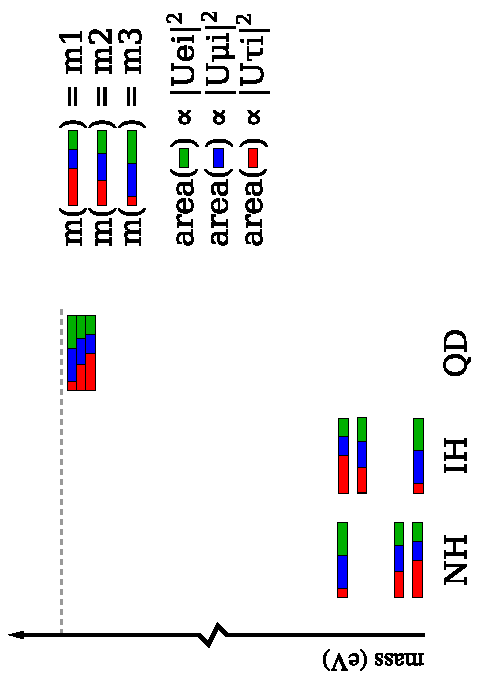
\includegraphics[height=0.8\textwidth,angle=-90]{figures/mass_scale.eps}
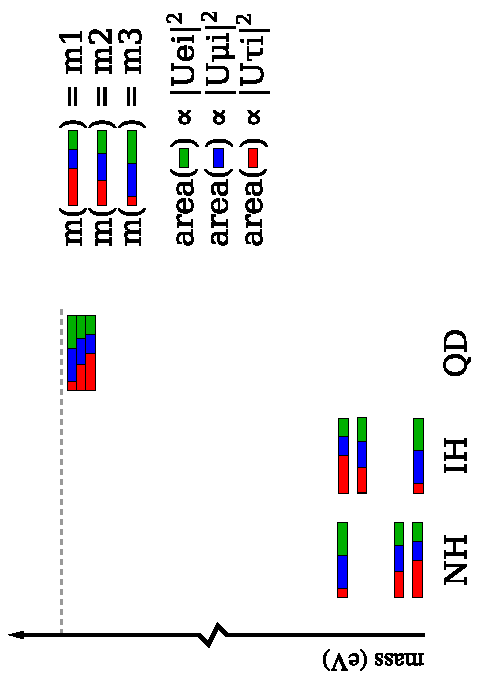
\includegraphics[width=0.8\textwidth]{figures/mass_scale.eps}
\caption[Neutrino mass hierarchies.]{The three possible mass hierarchies: normal hierarchy (NH), inverted hierarchy (IH), and quasi-degenerate (QD).  The dashed line indicates one-third the current limit for the absolute mass scale, $\sim\frac{2}{3}$~eV.}
\label{fig:massScale}
\end{figure}  

Long-baseline neutrino experiments have provided a comprehensive picture of neutrino mixing, but they cannot provide access to important information about the neutrino such as the absolute mass scale, CP-violating phases, or the origin of its small mass.  These will be discussed in the next section.


\section{Massive Neutrinos in the SM}
\label{sec:mass}
\begin{comment}
Discuss mechanisms by which neutrinos could get their mass.  
\end{comment}
In the standard model, fermions are four-component spinors that can be written in a chiral basis so that there is a ``left-handed'' component of the fermion $\psi_L$ and a ``right-handed'' component $\psi_R$, where $\psi_L$ and $\psi_R$ are two-component spinors.  The chiral basis is particularly useful because the weak bosons $W^{\pm}$ and $Z^0$ have been experimentally observed to only interact with the left-handed component of the fermion field.  The chiral basis is also helpful in understanding two possible ways to give neutrinos mass in the standard model.  Leptons acquire their mass by interacting with the Higgs field; the electron is the lightest because its coupling to the Higgs field is weaker than that of the muon.  The tau is strongly coupled to the Higgs field, making it the most massive of the leptons.  The diagram in {\fig}~\ref{fig:leptonMass} gives a heuristic picture of the lepton fields' interaction with the Higgs background.  
\begin{figure}[htp]
\centering
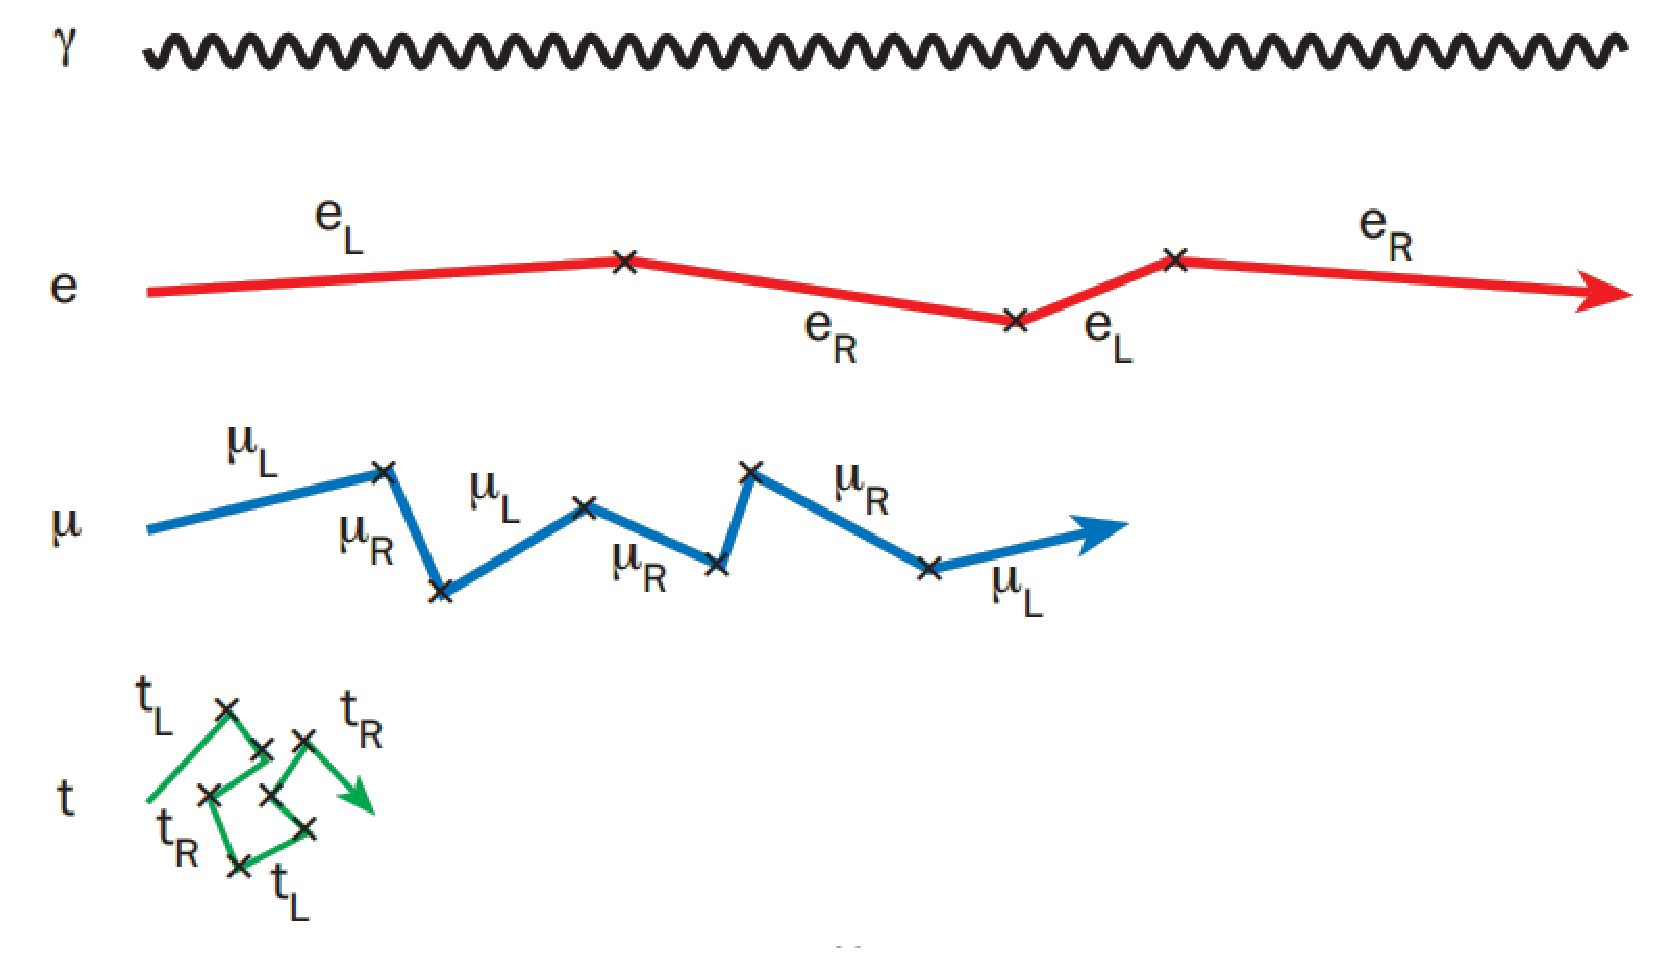
\includegraphics[width=0.8\textwidth]{figures/leptonMass.eps}
\caption[Lepton mass via the Higgs interaction.]{Leptons acquire mass by interacting with the Higgs field.  Vertices marked with $\times$ indicate an interaction with the background Higgs field.  The electron has a smaller coupling to the Higgs field than the tau and therefore interacts less.  In a Feynman diagram, lepton lines indicate already-massive leptons.  The lines here represent the  massless lepton fields and the entire diagram is analogous to a solid lepton line in a typical Feynman diagram.  Figure from {\refref}~\citep{neutrinoMass}.}
\label{fig:leptonMass}
\end{figure}
When neutrinos were thought to be massless, they were introduced into the SM as two-component spinor fields with no right-handed component.  The Higgs, which changes the chirality of the particle it interacts with, could not interact with the neutrino because it had no right-handed state to convert to.  The ansatz of a solely left-handed neutrino, then, created a massless neutrino in the SM.  As experimental evidence has overwhelmingly favored a massive neutrino, it became necessary to modify the theoretical treatment of the neutrino.  One approach is to assume that the neutrino, like the SM leptons, is a Dirac fermion and has a left-handed component as well as a right-handed component, allowing the Higgs field to interact with the neutrino as it does for the leptons.  There is another approach to generate massive neutrinos that is not solely dependent on the Higgs field.  If neutrinos are Majorana fermions, that is, if unlike Dirac fermions they are their own antiparticles, then the right-handed component of the neutrino field can introduce a mass term independent of the Higgs interaction.  When left-handed neutrinos interact with the background Higgs field, the right-handed neutrino with mass $M$ can only exist for a short time without violating the Pauli principle if $M$ is very large.  The right-handed neutrino quickly interacts with the Higgs background, transforming back into a left-handed neutrino.  The mass of the neutrino should then scaled by $m/M$, where $m$ is the mass due to interaction with the Higgs field.  See {\fig}~\ref{fig:neutrinoMass} for a picture of these different neutrino theories.  The advantage of the Majorana neutrino is that the scale of its interaction with the Higgs field can be comparable to that of other leptons; its small mass can be achieved by assuming a large $M$.  Majorana neutrinos are also attractive because a very massive neutrino could provide an explanation for the observed baryon asymmetry \citep{baryogenesis_Fukugita}.  
\begin{figure}[htp]
\centering
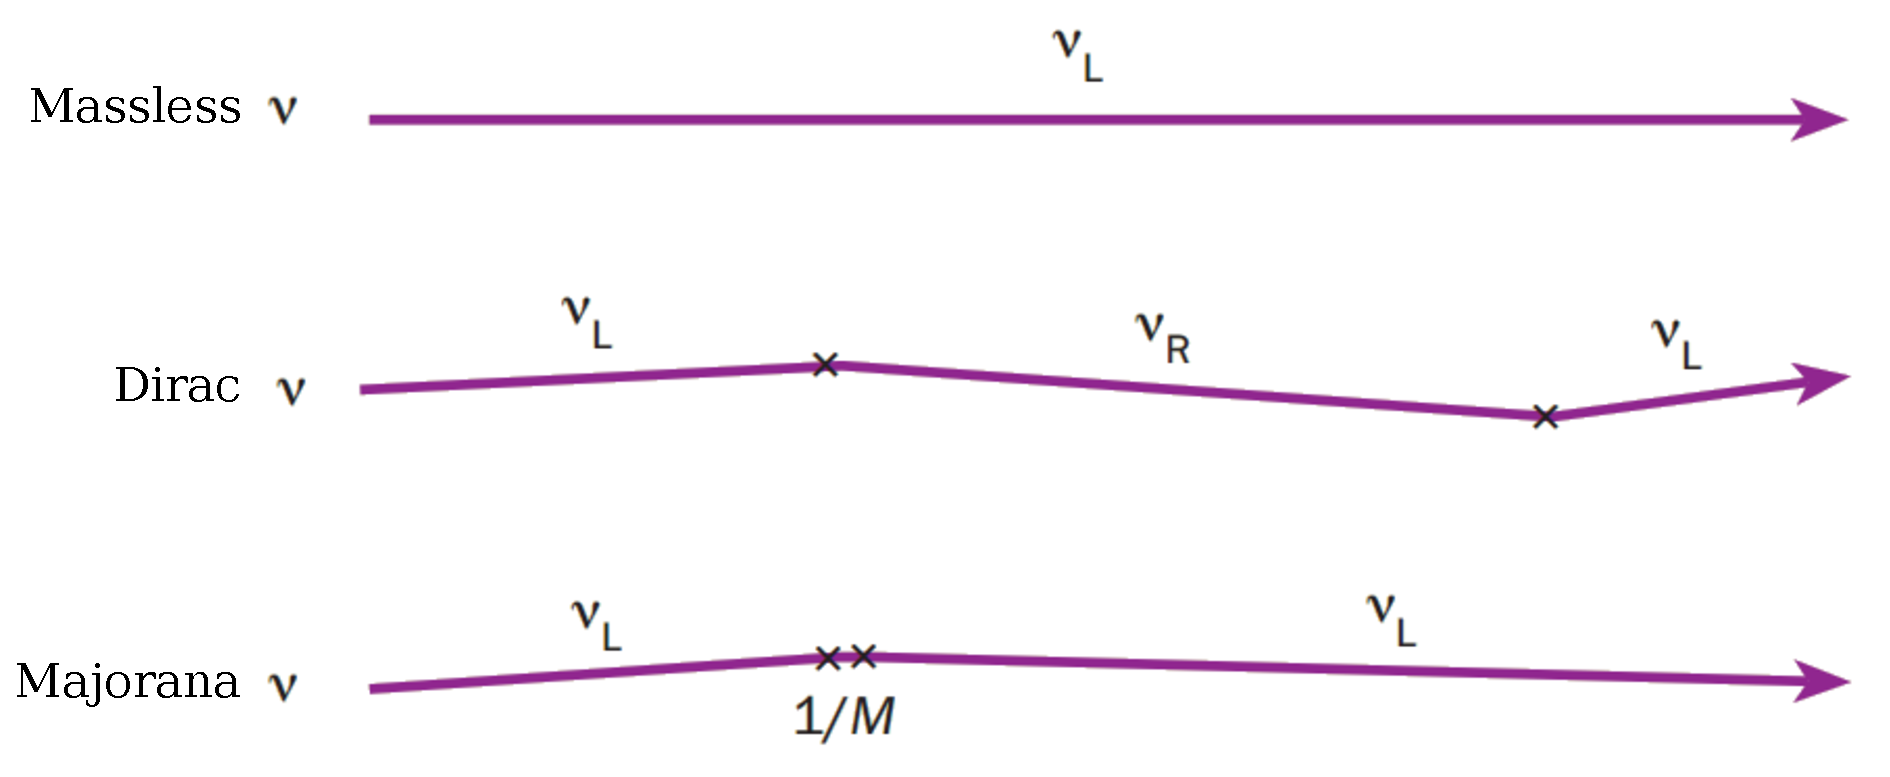
\includegraphics[width=0.8\textwidth]{figures/neutrinoMass.eps}
\caption[A depiction of massless, Dirac, and Majorana models of the neutrino.]{A representation of a massless neutrino, a Dirac neutrino, and a Majorana neutrino.  Vertices marked with $\times$ indicate an interaction with the background Higgs field.  Figure from {\refref}~\citep{neutrinoMass}.}
\label{fig:neutrinoMass}
\end{figure}  

Long-baseline experiments have determined that neutrinos are massive and have measured their mass differences and mixing angles, but much of their fundamental nature is still not understood.  That they could potentially play a significant role in many areas of physics provides significant motivation to build experiments that are sensitive to these neutrino ``parameters.'' One type of experiment that is sensitive to the Dirac or Majorana nature of the neutrino is a search for a process called neutrino-less double-beta decay (\zvbb).  Two-neutrino double-beta decay (\tvbb) is a process that has been observed for a number of nuclei and is the simultaneous beta-decay of two neutrons into two protons.  If the neutrino is a Majorana fermion, it would be possible for the neutrino to become an internal line in the Feynman diagram as shown in {\fig}~\ref{fig:zvbb}.  This process would be impossible if the neutrino were not its own antiparticle; observation of \zvbb would confirm the Majorana nature of the neutrino. 
\begin{figure}[htp]
\centering
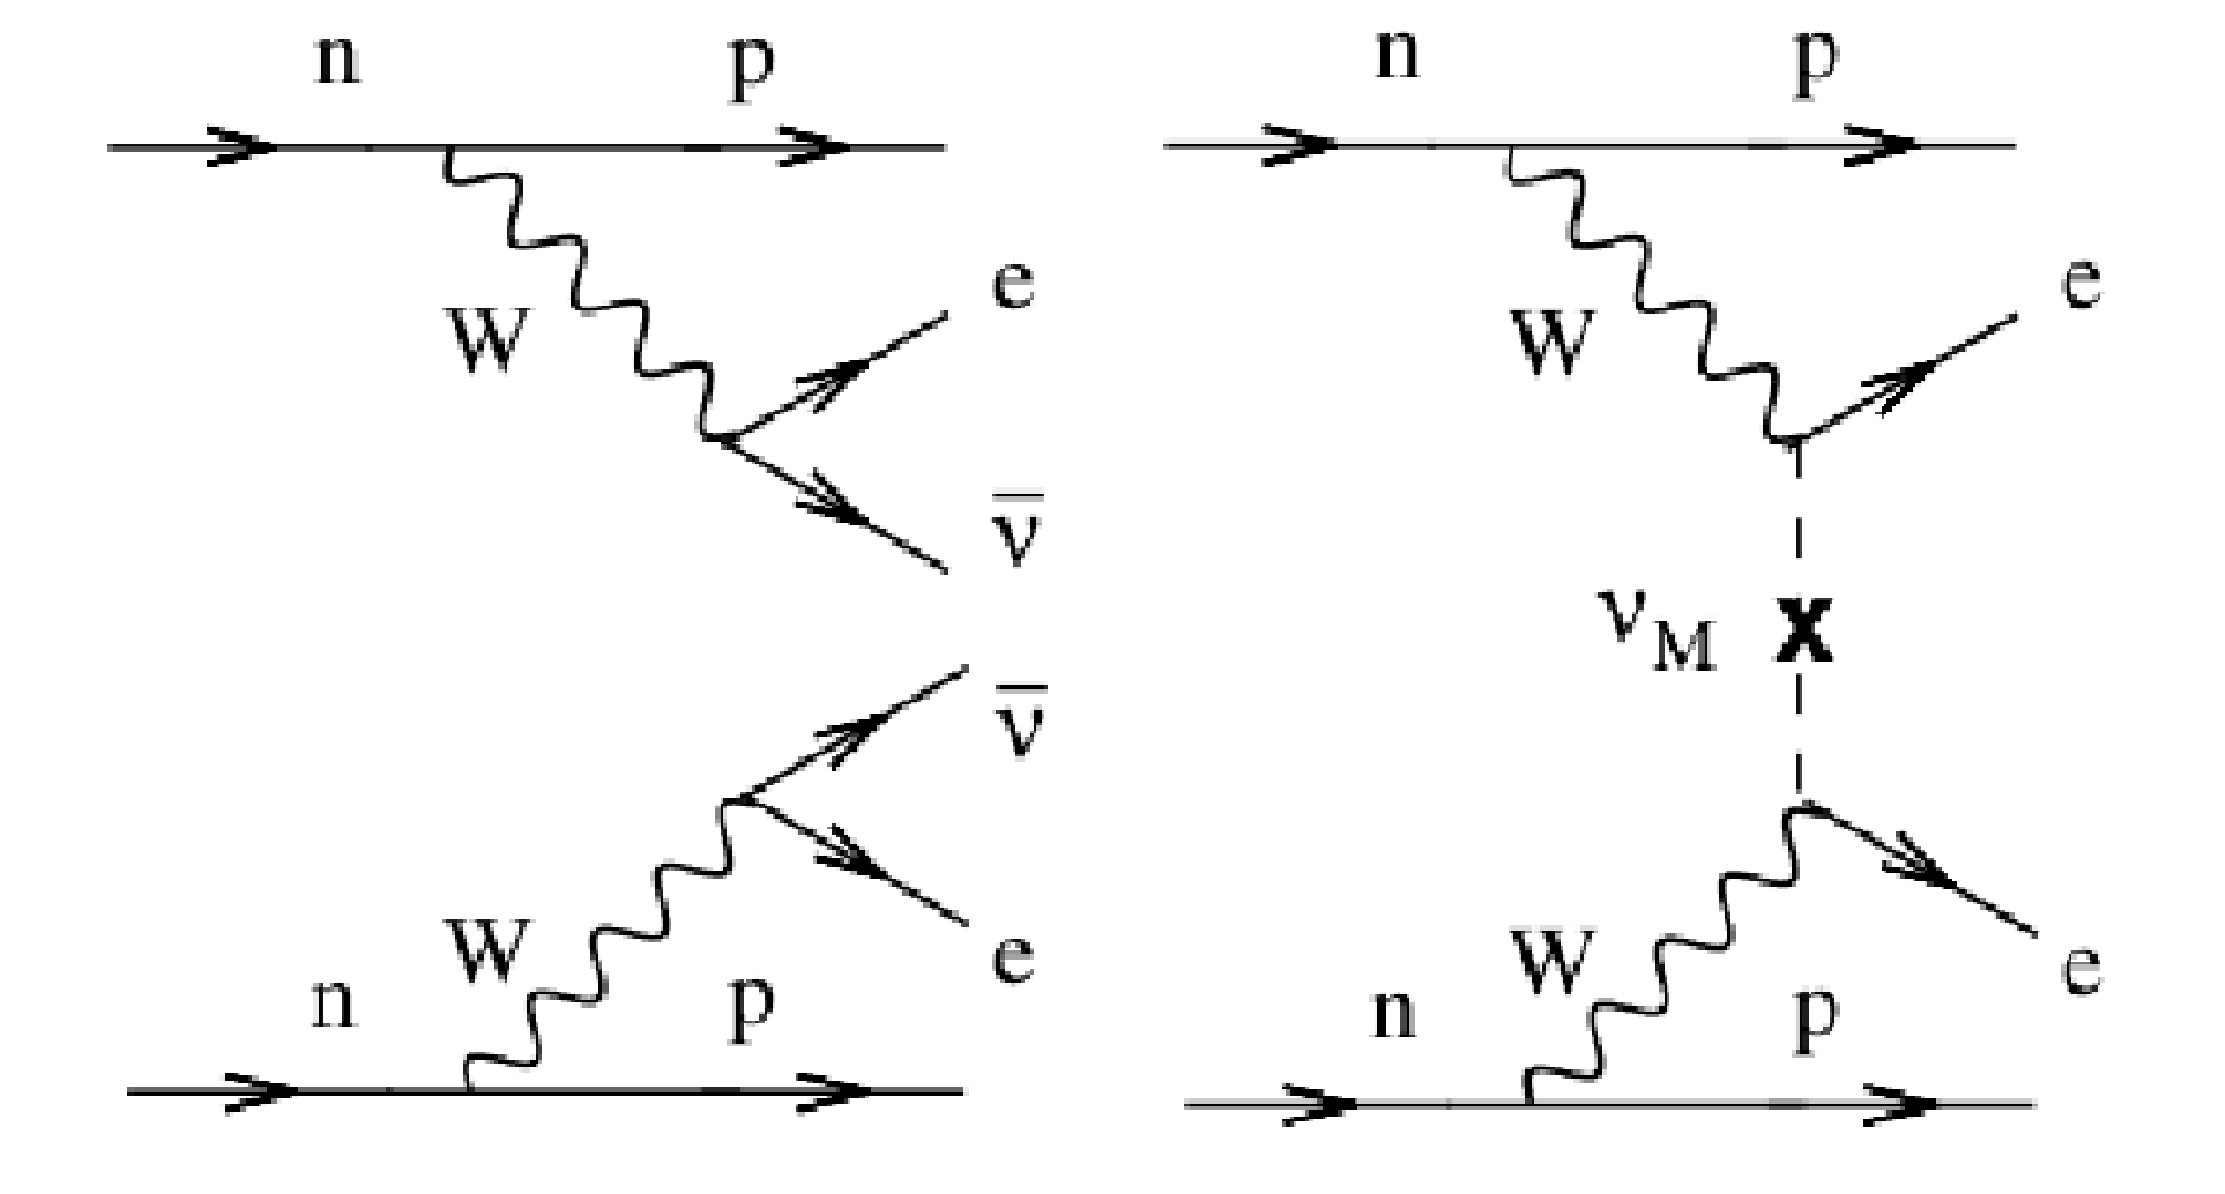
\includegraphics[width=0.8\textwidth]{figures/feynman2.eps}
\caption[Feynman diagrams describing \tvbb and \zvbb.]{Both the observed \tvbb (left) and the hypothesized \zvbb (right) modes are shown.  Nuclear matter is an ideal environment for spatially-close neutrons.  Figure from {\refref}~\citep{zvbbReview_Elliott}.}
\label{fig:zvbb}
\end{figure}
It should be noted that measured lifetimes for \tvbb are extremely long, on the order of $10^{20}$~yr.  The expected lifetime for \zvbb, if it exists, will be even larger due to the suppression of the right-handed component of the neutrino; the IGEX experiment places the current limit at $>1.57\times 10^{25}$~yr \citep{IGEX}.  This long lifetime makes \zvbb searches experimentally challenging.  However, they are currently the only way to explore crucial properties of the neutrino.  Aspects of these experiments are discussed in the next section.

\section{\zvbb searches}
\begin{comment}
Discuss \zvbb process and sensitivity to nature of neutrino.
Discuss concurrent sensitivity to hadron part
I feel like I should discuss ongoing searches but not in much detail?  Relevant information is: expected lifetime, mass, expected counts/year, expected limits?
Okay, yes.  Here is how this section could go: discuss the process and the resulting equation for the lifetime, and then talk about each of the components of the equation.  START with the discussion of the lifetime - can include details of ongoing experiments there.
\end{comment}

Searches for \zvbb are of interest not only because an observation would conclusively demonstrate that neutrinos are Majorana, but also because an observed rate gives information on the absolute mass scale of the neutrino.  The lifetime of \zvbb, assuming it results from the exchange of light Majorana neutrinos, is 
\begin{equation}
(T^{0\nu}_{1/2})^{-1} = G_{0\nu}(Q_{\beta\beta},Z)|M^{0\nu}|^2 {\langle}m_{\beta\beta}{\rangle}^2,
\end{equation}
where $G_{0\nu}(Q_{\beta\beta},Z)$ is a phase space factor, $|M^{0\nu}| = |{\langle}f|O|i{\rangle}|$, where $O$ is the \zvbb operator, is the nuclear matrix element, and $\displaystyle {\langle}m_{\beta\beta}{\rangle} \equiv |\sum_{i}m_i U_{ei}^2|$ is the effective Majorana mass.  The phase space factor can be readily calculated \citep{hadron_zvbb_Suhonen} and is typically on the order of $10^{-14}$~yr$^{-1}$.  The mass term is the effective mass of the electron neutrino and, unlike long-baseline experiments, is sensitive to the mass scale of the lightest neutrino particle.  This dependence is shown in {\fig}~\ref{fig:effectiveMajoranaMass} for the three possible hierarchy schemes.  
\begin{figure}[htp]
\centering
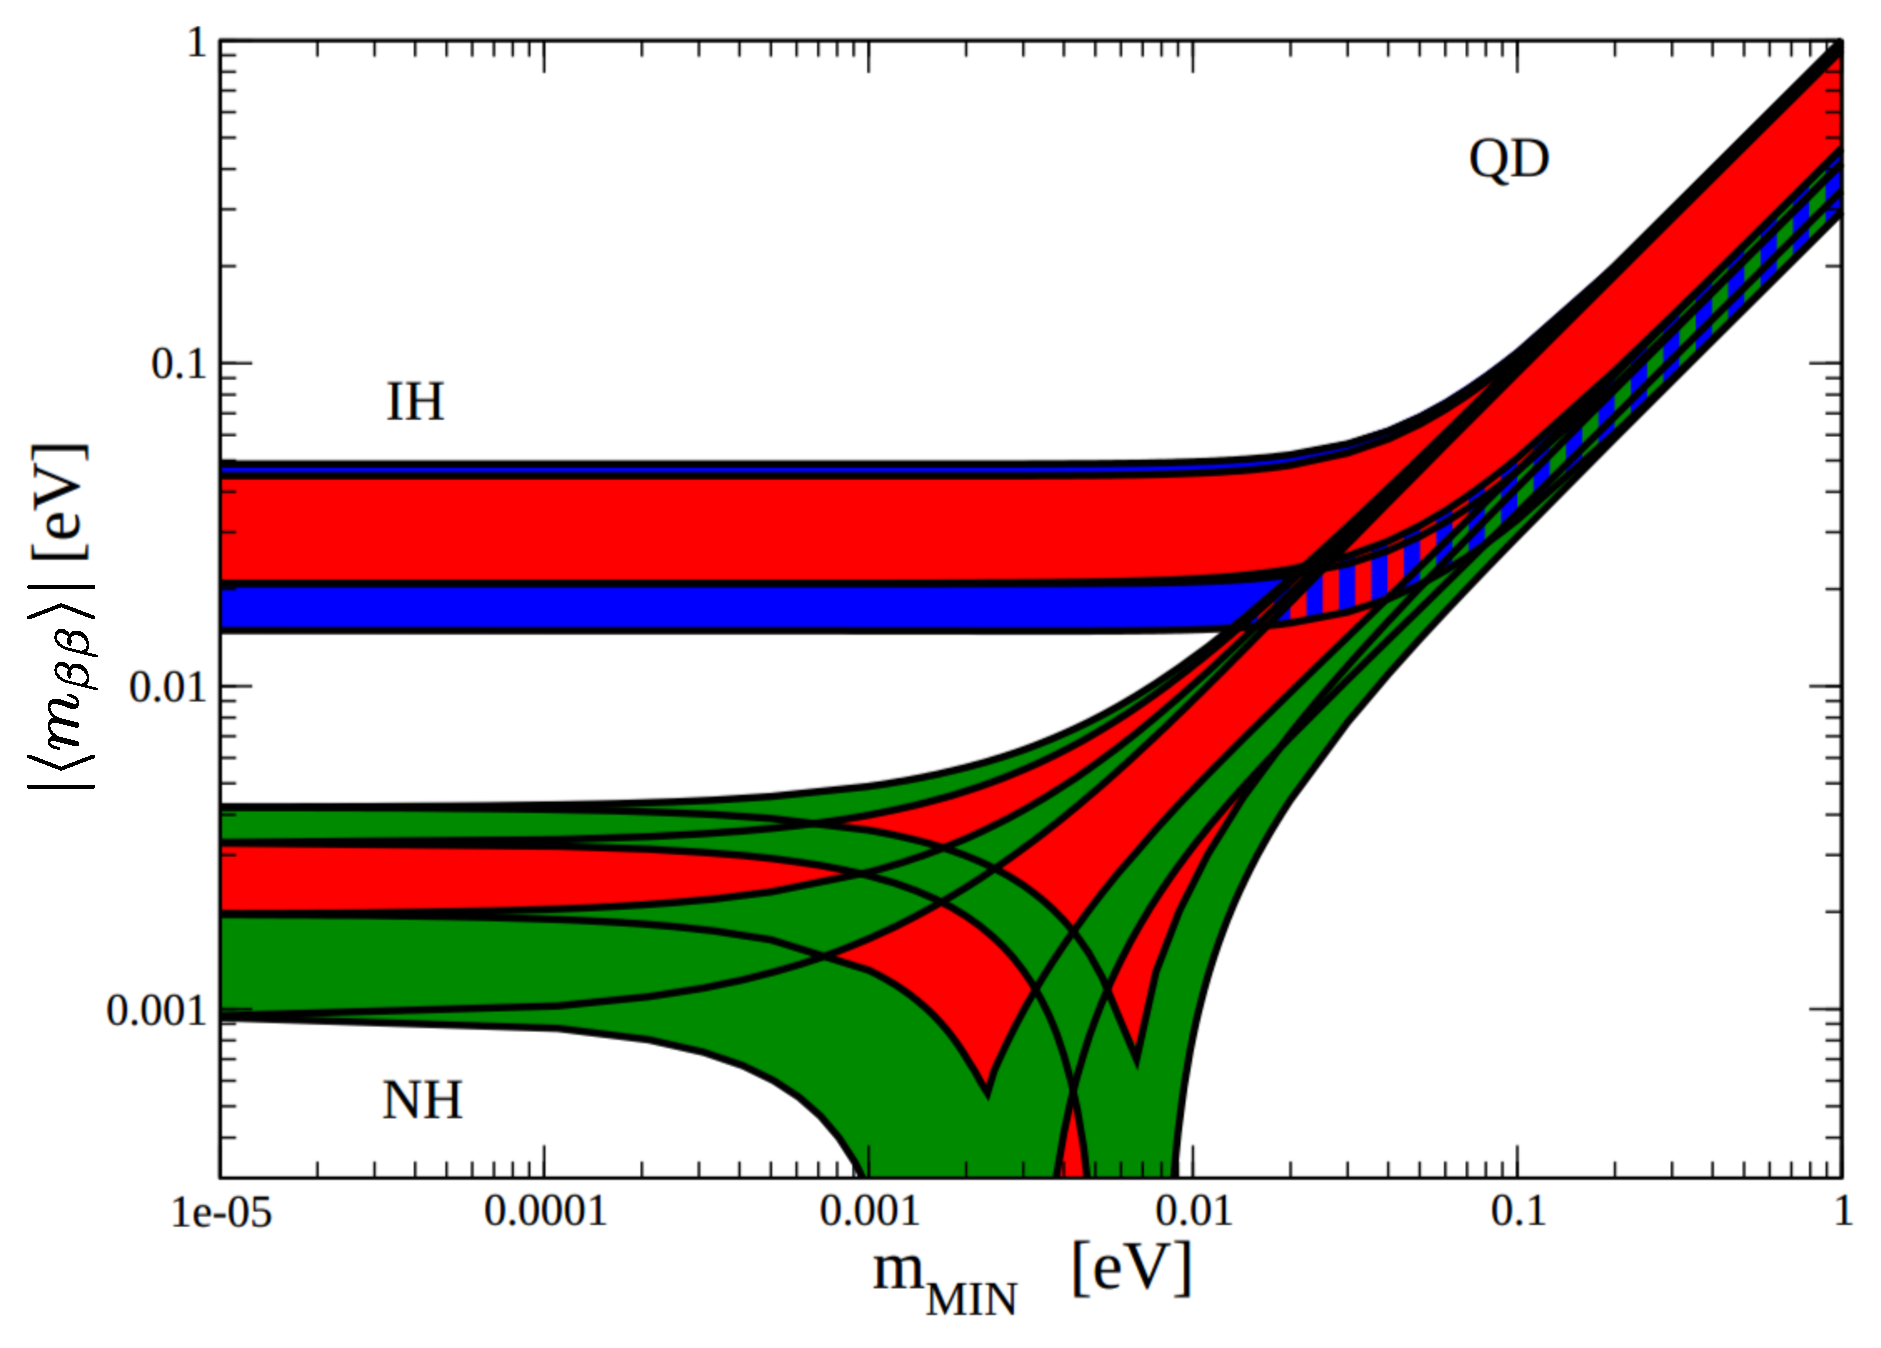
\includegraphics[width=0.8\textwidth]{figures/effectiveMajoranaMass.eps}
\caption[The effective Majorana mass as a function of the smallest neutrino mass.]{The effective Majorana mass as a function of the smallest neutrino mass $m_{min}$ for the inverse hierarchy (IH), normal hierarchy (NH), and quasi-degenerate (QD) scheme.  The values are shown in bands indicating the $2\sigma$ uncertainty.  For all values, it is assumed that $\sin^2{\theta}_{13} = 0.0236$ and $\delta = 0$.  Colors distinguish between different CP-violating scenarios of the Majorana phases.  Red bands require that $\alpha_{31}-\alpha_{21}$ as well as either $\alpha_{21}$ or $\alpha_{31}$ have a CP-violating phases.  Blue and green bands require that both $\alpha_{21}$ and $\alpha_{31}$ have CP-conserving phases.  Overlapping regions are shown hatched.  Figure from {\refref}~\citep{PDG}.}
\label{fig:effectiveMajoranaMass}
\end{figure}

The hadronic dependence of the lifetime, \NME, is sensitive to the initial and final nuclear wavefunctions.  Details of these calculations are discussed in {\chap}~\ref{chap:nucl}, but it should be noted that calculated \NME values for most candidate nuclei vary by as much as a factor of 5.
\begin{figure}[htp]
\centering
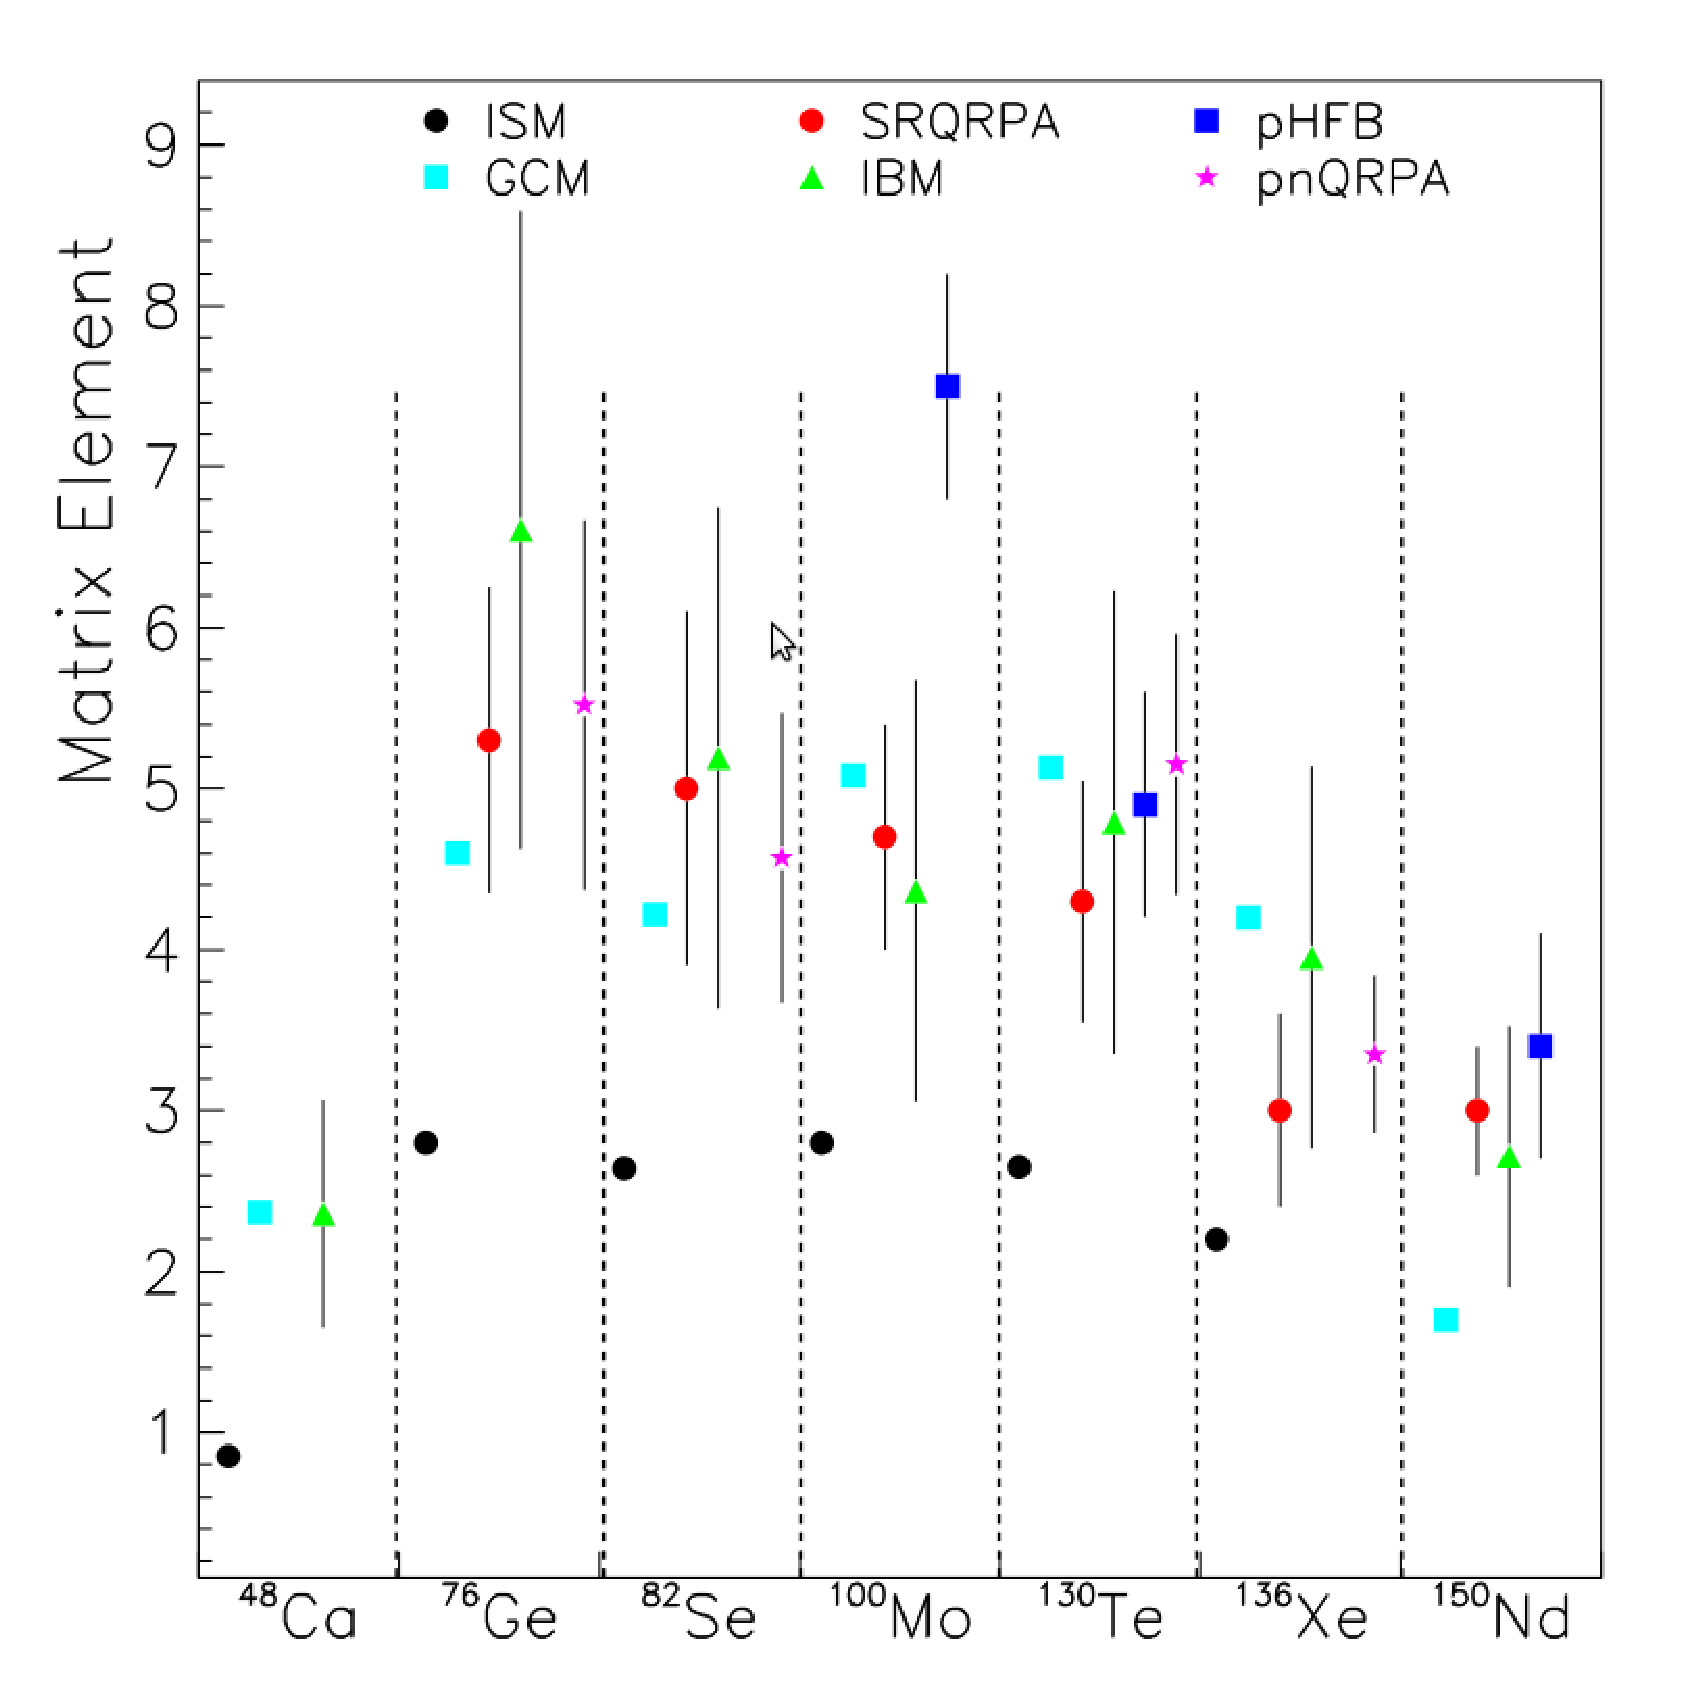
\includegraphics[width=0.8\textwidth]{figures/differentNME.eps}
\caption[Uncertainty in current calculated values of \NME.]{Calculated \NME for candidate \zvbb nuclei.  The models used for these calculations are the Interacting Shell Model (ISM) \citep{ISM}, self-consistent renormalized quasi-particle random phase approximation (SRQRPA) \citep{FaesslerReview}, proton-neutron quasi-particle random phase approximation (PNQRPA) \citep{pnQRPA_Suhonen}, generating coordinate method (GCM) \citep{GCM}, the interacting boson model (IBM) \citep{IBM_Iachello}, and the projected Hartree-Fock-Bogoliubov (pHFB) \citep{pHFB}.  Figure taken from \citep{zvbbReviewSchwingenheuer}.  Note that \NME is a dimensionless quantity; this is accomplished by multiplying by the nuclear radius, chosen here to be 1.2~fm.  For details on this quantity see {\ref}~\cite{}.}
\label{fig:differentNME}
\end{figure}  
This uncertainty in \NME directly affects the limits that can be placed on the neutrino mass scale if \zvbb is observed.  Transfer reactions, discussed in {\chap}~\ref{chap:nucl}, offer valuable experimental data that can be used to understand which models are most appropriate for these nuclei and improve the accuracy of the calculations.  The topic of this thesis is the two-proton transfer reaction, which is also discussed in {\chap}~\ref{chap:nucl}.

Nuclei that are suitable for \zvbb experiments are those that are stable against single beta decay but energetically allowed to double-beta decay.  This is the same group of nuclei in which \tvbb has been studied.  The \zvbb peak is at the endpoint of the \tvbb spectrum, and in fact the \tvbb process is a significant background to \zvbb due to finite detector resolution.  The nuclei $^{48}$Ca, \Ge{76}, \Se{82}, $^{100}$Mo, $^{130}$Te, $^{136}$Xe, and $^{150}$Nd have been used to search for the process in past and present experiments.  See {\tab}~\ref{tab:experiments} for a list of past and present experiments.  Because of the uncertainties on \NME for these nuclei (see {\fig}~\ref{fig:differentNME}, it is not clear which, if any, would enjoy a shorter $T^{0\nu}_{1/2}$.  So many different experiments have arisen because each candidate nucleus offers different advantages in experimental design.  \Ge{76} is an appealing candidate because the active volume also serves as the detector, and Ge crystals are well understood.  Experiments using \Ge{76} are also important because the Heidelberg-Moscow experiment, which claimed an observed \zvbb signal \citep{KlapdorKleingrothaus}, used \Ge{76} crystals.  Other nuclei are appealing because they have high abundance or are easy to obtain.  This is the case for $^{136}$Xe, which is currently being used by the EXO-200 collaboration \citep{EXO200}.  Experiments using $^{136}$Xe typically use time projection chambers (TPC's), which are able to strongly reduce background by reconstructing the momenta of particles in a decay.  Using $^{136}$Xe is particularly appealing because large quantities are readily available, reducing the cost of increasing the mass scale of the experiment.  Another candidate nucleus, $^{130}$Te, is frequently used in experiments using bolometry to detect \zvbb.  A summary of \zvbb searches is shown in {\tab}~\ref{tab:experiments}.
\begin{sidewaystable}
\ra{1.1}\small
\centering
\caption[\zvbb \uppercase{experiments}]{\\\zvbb \uppercase{experiments}}
\label{tab:experiments}

\begin{tabular}{@{}rlllllll@{}}\toprule
\multicolumn{1}{l}{Experiment} & Isotope & Mass [kg] & Method & $T^{2\nu}_{1/2}$ [yr] & $T^{0\nu}_{1/2}$ [yr] & Start - End & {\refref} \\
\midrule
\multicolumn{1}{l}{\textbf{Past Experiments}} \\
Heidelberg-Moscow & \Ge{76} & 11 & ionization & $(1.74\pm0.18)\times 10^{21}$ & $1.19^{+2.99}_{-0.5}\times 10^{25}$ &1990 - 2003 & \citep{KlapdorKleingrothaus} \\
Cuorcino & $^{130}$Te & 11 & bolometer & & $> 2.8\times 10^{24}$ & 2003 - 2008 & \citep{Cuorcino} \\
NEMO-3 & $^{100}$Mo & 7 & track + calorim. & $(0.716\pm0.055)\times 10^{19}$ & $> 1.0\times 10^{24}$ & 2003 - 2009 & \citep{NEMO3} \\
NEMO-3 & $^{82}$Se & 1 & track + calorim. & $(9.6\pm1.1)\times 10^{19}$ & $> 3.2\times 10^{23}$ & 2003 - 2009 & \citep{NEMO3} \\
\noalign{\vskip 0.3cm}

\multicolumn{1}{l}{\textbf{Current Experiments}} \\
EXO-200 & $^{136}$Xe & 175 & liquid TPC & $(2.1\pm0.2)\times 10^{21}$ & $>1.6\times 10^{25}$ & 2011 - & \citep{EXO200} \\
Kamland-Zen & $^{136}$Xe & 330 & liquid scint. & $(2.38\pm0.14)\times 10^{21}$ & $>5.7\times 10^{24}$ & 2011 - & \citep{KamLAND_Zen} \\
GERDA-I/GERDA-II & \Ge{76} & 15/35 & ionization & $(1.88\pm0.1)\times 10^{21}$ & & 2011/2013 - & \citep{Gerda} \\
CANDLES & $^{48}$Ca & 0.35 & scint. crystal & & & 2011 - & \citep{CANDLES} \\
\noalign{\vskip 0.3cm}

\multicolumn{1}{l}{\textbf{Funded Experiments}} \\
NEXT & $^{136}$Xe & 100 & gas TPC & & & 2015 - & \citep{NEXT} \\
Cuore0/Cuore & $^{130}$Te & 10/200 & bolometer & & & 2012/2015 - & \citep{Cuore} \\
Majorana Demo & \Ge{76} & 30 & ionization & & & 2013 - & \citep{Majorana} \\
SuperNEMO Demo & \Se{82} & 7 & track + calorim. & & & 2014 - & \citep{SuperNEMO} \\
SNO+ & $^{150}$Nd & 44 & liquid scint. & & & 2013 - & \citep{SNO} \\
\bottomrule
\end{tabular}
\begin{flushleft}
\small NOTE:
Past, present, and future \zvbb experiments.  Detecting a signal in several different isotopes would greatly improve the likelihood of a Majorana process.  From \citep{zvbbReviewSchwingenheuer}.
\end{flushleft}
\end{sidewaystable}

Searches for \zvbb offer access to unique areas of neutrino physics.  Confirmation of the process would demonstrate that neutrinos are Majorana in nature and would also provide a measurement of the absolute mass scale of the electron neutrino.  The dependence of the lifetime on \NME poses a difficulty because the current uncertainty in calculations limits the sensitivity to the neutrino mass scale and also increases the difficulty of planning experiments that search for the process.  Nuclear transfer experiments provide information that can help reduce the uncertainty of \NME calculations, and this thesis focuses on two-proton transfers in the Ge nuclei.  The impact of such a transfer experiment is discussed in {\chap}~\ref{chap:nucl}.


% % uncomment the following lines,
% if using chapter-wise bibliography
%
% \bibliographystyle{ndnatbib}
% \bibliography{example}



%
% Chapter 2
%

%
% Modified by Sameer Vijay
% Last Change: Wed Jul 27 2005 13:00 CEST
%
%%%%%%%%%%%%%%%%%%%%%%%%%%%%%%%%%%%%%%%%%%%%%%%%%%%%%%%%%%%%%%%%%%%%%%%%
%
% Sample Notre Dame Thesis/Dissertation
% Using Donald Peterson's ndthesis classfile
%
% Written by Jeff Squyres and Don Peterson
%
% Provided by the Information Technology Committee of
%   the Graduate Student Union
%   http://www.gsu.nd.edu/
%
% Nothing in this document is serious except the format.  :-)
%
% If you have any suggestions, comments, questions, please send e-mail
% to: ndthesis@gsu.nd.edu
%
%%%%%%%%%%%%%%%%%%%%%%%%%%%%%%%%%%%%%%%%%%%%%%%%%%%%%%%%%%%%%%%%%%%%%%%%

%
% Chapter 2
%

\chapter{TRANSFER REACTIONS AND NUCLEAR MATRIX ELEMENTS}
\label{chap:nucl}

The NME for the \tvbb process are well-understood, but calculation of \NME for the \zvbb process is significantly different \cite{VogelReview}.  This chapter discusses the calculation of \NME for the \zvbb process and the constraints that can be placed on these calculations with experimental data, including the two-proton transfer data that is the topic of this thesis.  The model of the nucleus as a collection of independent particles underlies all further discussions of \NME and interpretation of experimental results and is discussed first.    

\section{Shell Model of the Nucleus}
\begin{comment}
Using H.O. eigenstates to describe nucleons.
\begin{itemize}
\item nuclear potential well - is this something we can understand independently?  Certainly the radius is.
\item solutions to finite square well in terms of H.O. eigenstates and a diagram of energy levels
\item the energy levels give correct shell closures when spin-orbit coupling is introduced
\item so H.O. eigenstates are a reasonable way to describe nucleons
\end{itemize}

Looking at the valence nucleons to understand the whole nucleus.
\begin{itemize}
\item and because the nucleons couple so strongly into \zp pairs, describing the unpaired nucleons often accurately describes the entire nucleus
\item give a simple example?  \He{3} might be useful?
\item show level filling for \Ge{74} (32 protons) and point out the valence nucleons are f, p, g
\end{itemize}
\end{comment}

Trends in systematic nuclear data such as nuclear mass give clear evidence of ``magic numbers'' of protons and neutrons in nuclei, suggesting a central potential similar to that felt by electrons orbiting an atom.  One could perhaps determine the likely shape of the nuclear central potential by finding one that accurately reproduced the magic numbers.  One model that has promising beginnings is the harmonic oscillator potential.  To determine the magic numbers predicted by this potential, consider the quantum numbers that describe an eigenstate of this potential.  The principal quantum number, $n$, indicates the number of nodes of the state.  In this work, the node at infinity is included rather than the node at zero, so that $n$ ranges from 1 to $\inf$.  The orbital angular momentum is denoted $l$, with $l = 0, 1, 2, 3, ...$ typically called the $s, p, d, f, ...$ orbitals as in atomic electron structure.  The eigenvalue associated with the projection of the orbital angular momentum operator along the $z$-axis is $m$, which varies between $-l$ and $l$ and is called the magnetic quantum number.  The eigenvalues of any eigenstate of a spherically symmetric potential cannot depend on the magnetic quantum number, so that for the harmonic oscillator potential, any state associated with $l$ has a multiplicity of $2(2l+1)$, where the additional factor of two is due to nucleons being spin-1/2 fermions.  The eigenvalues of the three-dimensional harmonic oscillator are $E_{nl} = (2n+l-\frac{1}{2})\hbar\omega$, so that the energies proceed in uniform steps as $2n+l$ increases by one unit.  {\fig}~\ref{fig:shellModelMagic} shows the level spacing for this potential; note that the energy levels are multiplets.  For example, the states $nl = 2s$ and $1d$ both have energy $\frac{3}{2}\hbar\omega$.  
\begin{figure}[htp]
\centering
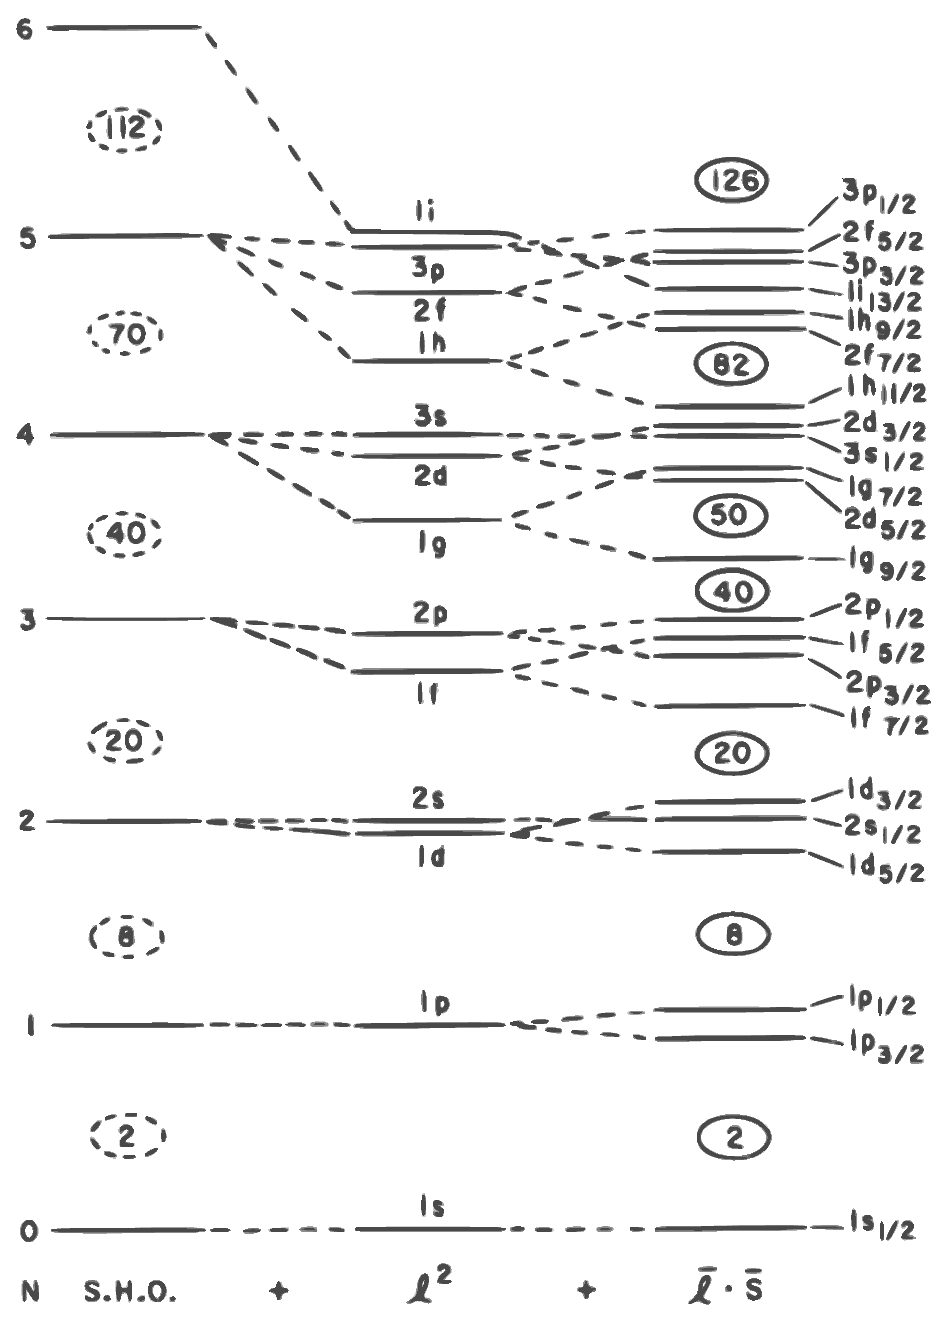
\includegraphics[width=1.0\textwidth]{figures/nuclearLevels.eps}
\caption{From \cite{Casten}.}
\label{fig:shellModelMagic}
\end{figure}
The harmonic oscillator potential predicts magic numbers at 2, 8, 20, 40, 70, and 112.  This matches the observed pattern for low numbers but begins to deviate for heavier nuclei.  A reasonable correction to make to the potential is to make it more uniform to more accurately reflect the fact that the density of nuclei is quite uniform \cite{Casten}.  Introducing a potential term proportional to $l^2$ does this by reducing the potential near the center of the well (where the orbital angular momentum is smaller) and increasing the potential further from the center, where the orbital angular momentum is larger.  Adjusting the potential in this way splits the $l$-degeneracy of the states but does not fundamentally change the predicted magic numbers.  It was not until Maria Goeppert-Mayer added a spin-orbit term to the potential \cite{MGM} that these magic numbers were correctly reproduced.  

An useful concept in nuclear structure is that of the valence shell of a nucleus.  Nucleons in a filled shell form a $J=0$ core that can be considered largely inert, while the remaining nucleons occupy the valence shell.  The picture is even further simplified due to the strong tendency for nucleons to couple into $J=0$ pairs, so that the ground state of a nucleus can be described simply by describing its unpaired nucleons.  The nucleus of primary interest in this work, \Se{76}, has 34 protons and 42 neutrons.  Like all even-even nuclei, its ground states is \zp, evidencing the strong coupling of nucleons into $J=0$ pairs.  The nucleons studied by ($^3$He,n) transfer are proton-pair holes; the valence shells of \GeTargets are predicted to be $2f_{5/2}$.  While the phenomenological potentials discussed above reproduce trends in nuclear data with great accuracy, the exact wavefunctions of \GeTargets are not known and it can at best be said that the $f$, $p$, and $g$ orbitals are expected to be the primary components of the ground-state wavefunction.  Because the \NME depends on the overlap between the initial and final nuclei, it is desirable to understand these nuclei, and particularly the differences between their ground states, as accurately as possible.  A series of experiments were undertaken to understand these wavefunctions more accurately and will be discussed in {\sect}~\ref{sec:valence,sec:correlations}.

\section{Calculation of \NME and Experimental Constraints}

One approach to calculating \NME = $\langle f||O||i \rangle$ is with the shell-model formalism described above.  The difficulty with this approach is that the \zvbb process is spatially confined to $\sim$2-3~fm, which means that intermediate states with momentum up to $\sim$100~MeV \cite{anatomy} are relevant to the calculation.  Even though expressing these states with a shell-model basis set can require a space as large as $O(10^{10})$,  several groups have still undertaken this method of calculating \NME \cite{CaurierShellModel}.  Regardless of the method of calculation, the wavefunctions of the initial and final nuclei must impact \NME.  Extensive single-nucleon transfer experiments have been performed to better understand the valence shells and are discussed further in {\sect}~\ref{sec:valence}.

A more common approach to the calculation of \NME is the Quasi-Particle Random-Phase Approximation (QRPA).  The QRPA is a density functional theory that provides a framework particularly suited for describing collective excitations \cite{Casten}.  QRPA assumes that the ground state of the nucleus is in a fully-paired state \cite{BenderSCMF} similar to that in descriptions of superconductivity described by Bardeen, Cooper, and Schreiffer (BCS) [CITE].  The BCS ground state for even-even nuclei was first suggested by Bohr and Mottelson \cite{nucleiBCS} and is still considered a good approximation for many nuclei [CITE].  It is known, however, that the assumption of BCS symmetry of the nuclear ground state can be broken by deformation as well as large gaps between shells that can result in pairing vibrations [CITE].  In these cases, QRPA calculations can be inaccurate.  Two-nucleon transfer experiments can be helpful in determining the distribution of pairing strength in a nucleus \cite{Yoshida} and therefore confirm the validity of the QRPA assumptions in a nucleus or suggest further examination.  See {\sect}~\ref{sec:correlations} for more details on the effect of nuclear correlations on the calculation of \NME. 

\section{Valence Shells of the Initial and Final Nuclei}
\label{sec:valence}
\begin{comment}
\subsection{NME calculations and valence States}
\begin{itemize}
\item (assume that) NME calculations are sensitive to occupied valence states
\item can investigate valence state occupation with transfer reactions
\item \Ge{76} occupancies were experimentally determined and adjusting the energy levels to match changed the NME by a factor of 2 \cite{0vbbReview}
\end{itemize}
\end{comment}
As discussed in {\chap}~\ref{chap:0vbb}, the half-life of the \zvbb process depends on the nuclei as well as the neutrino mass scale.  While a direct measurement of \NME = $\langle f||O||i \rangle$ is difficult because it is only directly accessible by observation of \zvbb, it is possible to study the initial and final nuclear states separately in an attempt to improve the accuracy of the calculation.  Comprehensive single-nucleon transfer experiments have been performed on many of the candidate nuclei; see \cite{schiffer_review} for an overview of current progress.  Single-nucleon transfer is an important tool because it is sensitive to the difference between the occupancy of valence nucleons in the initial and final states.  Very generally, the cross-section for transferring a nucleon to a specific state in a target nucleus will be high if that nucleus has many holes available in that state but low if that state in the nucleus is filled.  Macfarlane and French \cite{sumRules} calculate the summing rules that allow determination of valence shell occupancies and vacancies from experimental transfer data.  The valence neutrons in the candidate nucleus \Ge{76} and its daughter \Se{76} have been studied with the neutron-adding reactions (d,p) and ($\alpha$,\He{3}) as well as neutron-removing reactions (p,d) and (\He{3},$\alpha$) \cite{valenceNeutrons}.  The valence protons of these same nuclei have been studied with the (d,\He{3}) reaction \cite{valenceProtons}.  These studies were also done on the \Ge{74} and \Se{74} nuclei for a consistency check and demonstrated that the Fermi surface of both the protons and neutrons in \GeTargets are quite diffuse, with the relevant neutron and proton orbits being 2$p_{3/2}$, 1$f_{5.2}$, 2$p_{1/2}$, and 1$g_{9/2}$.  The quantities most important to the NME calculations are the differences in occupancies between the mother and daughter nucleus; these differences are shown in {\fig}~\ref{fig:occupancyDiffs} along with the theoretical predictions.
\begin{figure}[!htbp]
\centering
\subfloat[][]{
   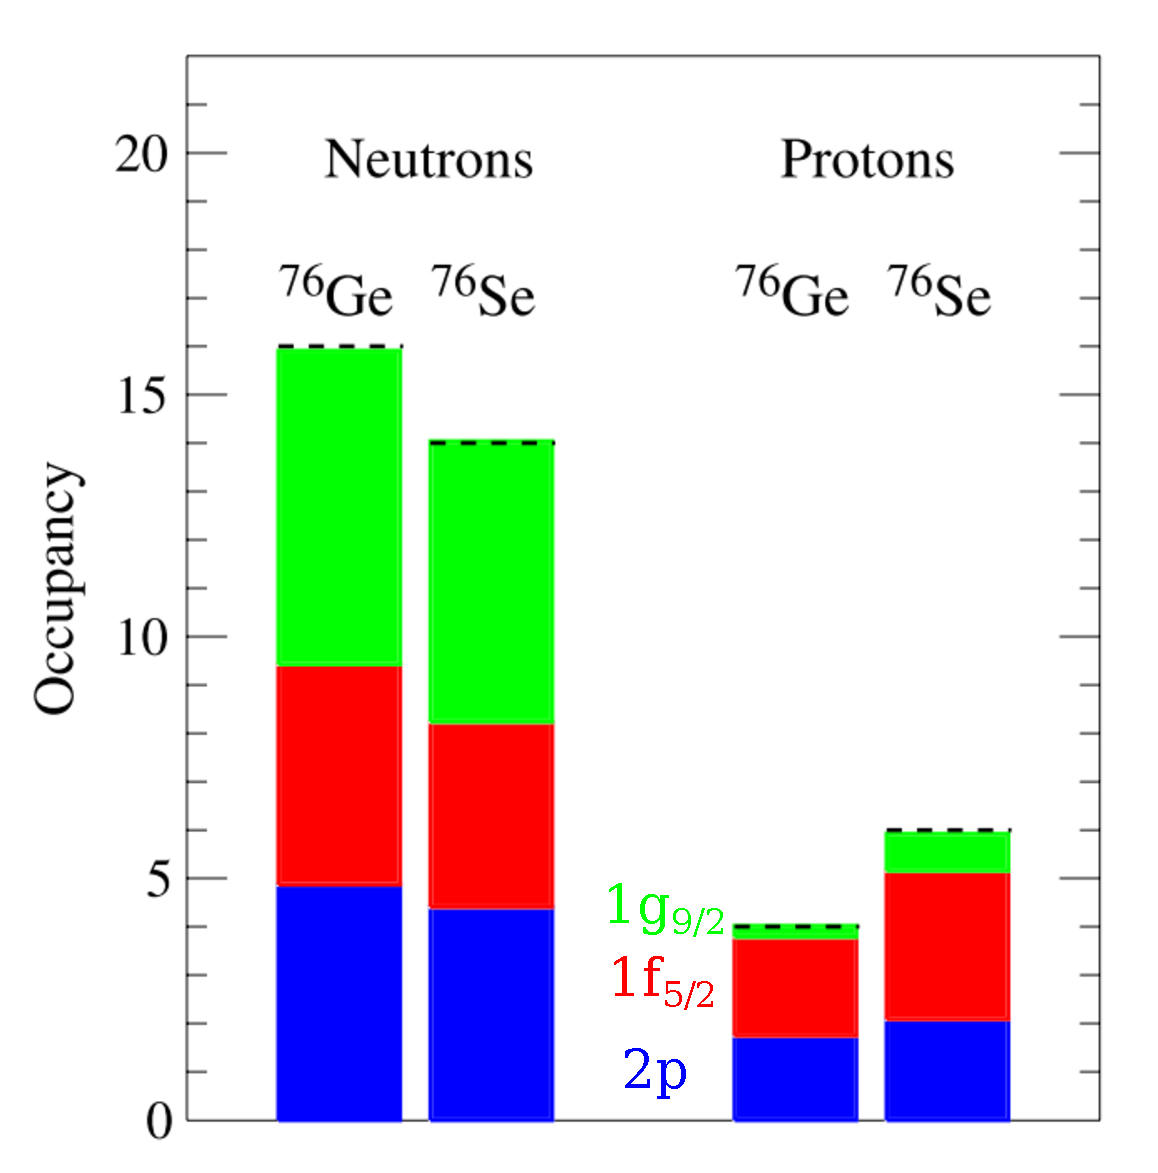
\includegraphics[width=0.4\textheight]{figures/occupancies.eps}
}
\subfloat[][]{
   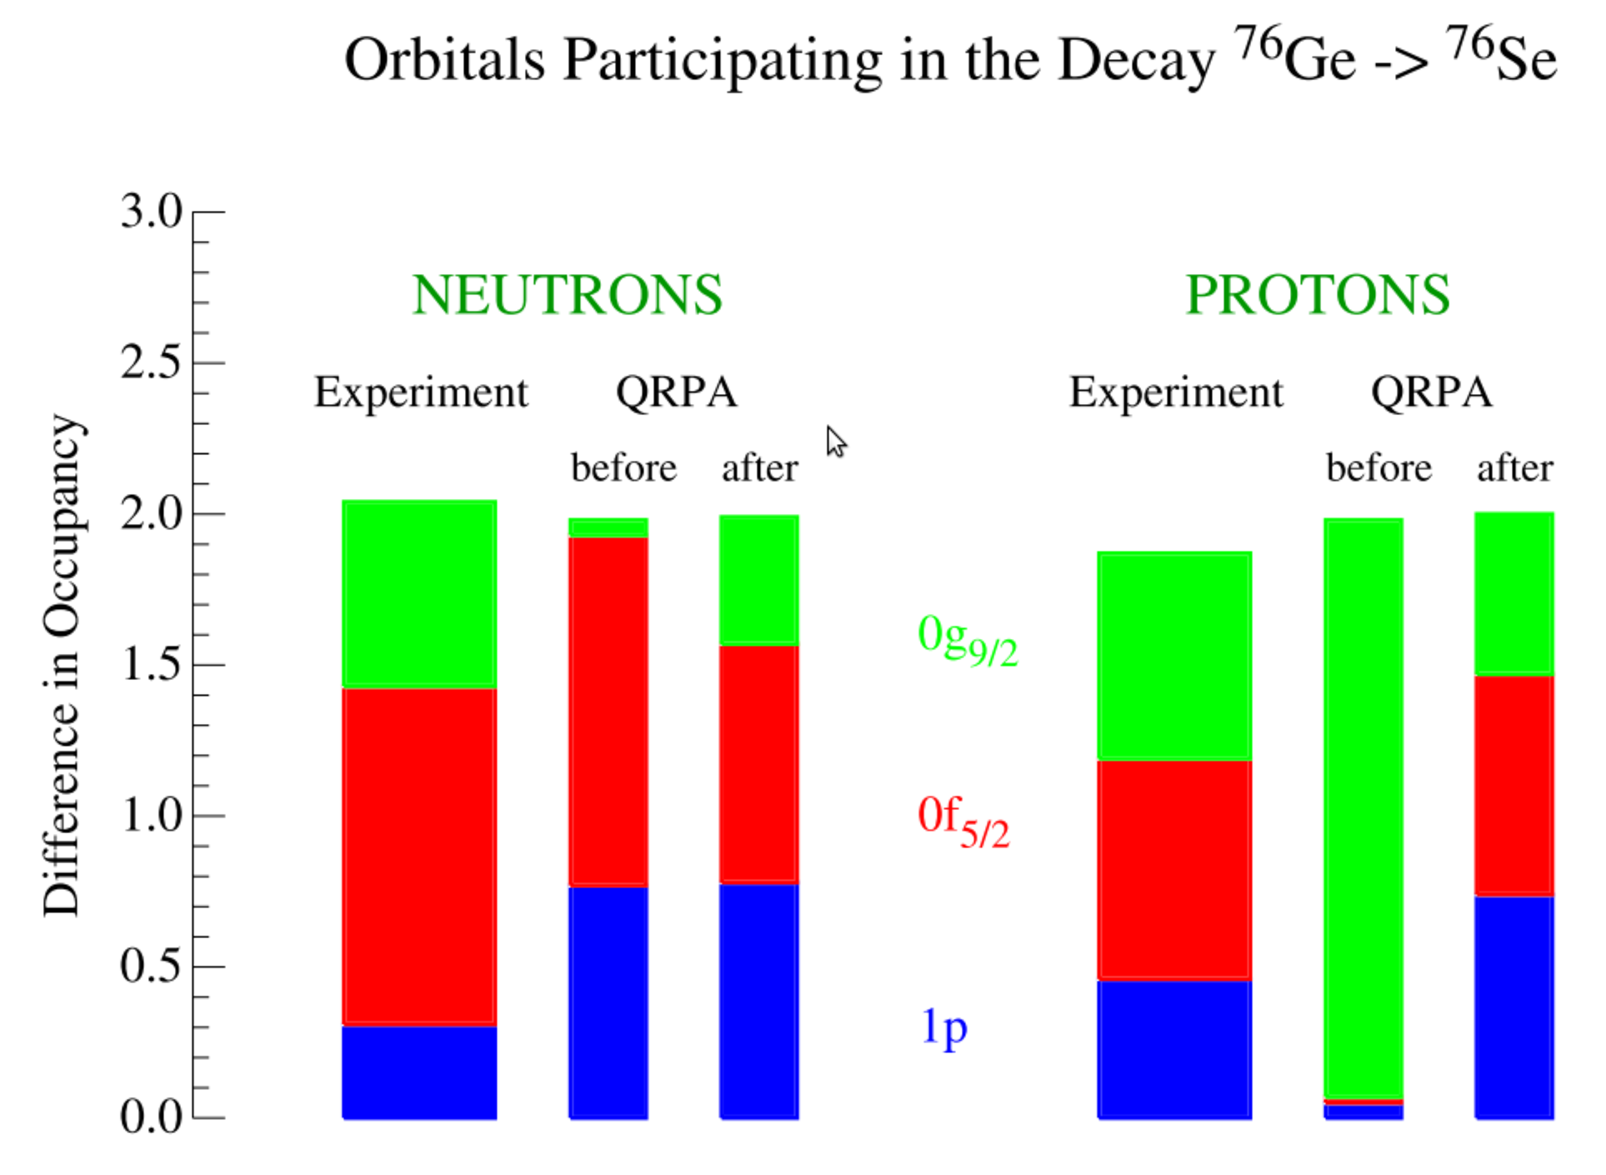
\includegraphics[width=0.5\textheight]{figures/occupancyDiffs.eps}
}
\caption{(a) Occupancies of the neutron and proton valence shells of \Ge{76} and \Se{76} determined by single-nucleon transfer reactions.  From \cite{schiffer_review}.  (b)  The differences between occupancies in the final and initial states are determined from (a) and are more immediately relevant to \NME calculations.  The theoretical predictions, before and after adjusting level energies to better match the data, are shown next to the experimental values.  From \cite{schiffer_review}.}
\label{fig:occupancyDiffs}
\end{figure}
The single-particle energy levels were adjusted in the QRPA calculation \cite{SuhonenEnergyAdjust} to provide better agreement with the data.  These changes reduced the QRPA calculation of \NME by approximately a factor of two, bringing it into agreement with the shell-model calculation of \NME.  This reduction in the spread of calculated \NME is particularly valuable to reducing the uncertainty of mass limits or estimates from \zvbb searches. 

\section{Nucleon-nucleon correlations and the impact they have on NME}
\label{sec:correlations}
\begin{comment}
\begin{itemize}
\item \zvbb occurs on correlated neutron pairs
\item certain pairing in the nucleus can inhibit \zvbb
\item investigate pair correlation with two-nucleon transfer reactions
\item some systems don't have all their \zp in the ground state - Xe
\item discuss neutron transfer experiments done on \GeTargets
\item wish to investigate proton transfer on \GeTargets
\end{itemize}
\end{comment}
In addition to studying the single-nucleon states in \GeTargets and \SeProducts, understanding correlated neutron pairs in \Ge{76} and correlated proton pairs in \Se{78} is relevant to \NME.  Calculations suggest that significant contributions to \NME come from inter-nucleon distances of less than 3~fm \cite{anatomy}.  The distribution of highly-spatially-correlated \zp strength, therefore, may strongly influence \NME.  QRPA calculations can be particularly sensitive to \zp strength that is not exclusively in the ground state as these models assume a BCS approximation where the ground state contains all \zp strength \cite{BenderSCMF}. 

Pair-transfer reactions such as (p,t) and (\He{3},n) are useful probes of pairing in nuclei as the cross-section for \zp states is dramatically forward peaked and therefore distinct \cite{Yoshida}.  The cross section of a two-nucleon transfer reaction on a nucleus that is well described by BCS should show strong population of the \zp ground-state with little, if any, population of \zp excited states.  A system that demonstrates the motivation for studying pairing in \Ge{74} particularly well is $^{128,130}$Te.  The neutron-pair adding reaction (p,t) was used to show that the cross section for excited \zp states is less than 4\% of that for the ground-state \zp cross section \cite{neutronPairsTellurium}, suggesting that BCS symmetry is a reasonable approximation for the neutrons in $^{128,130}$Te.  The same is not true for the proton states; the (\He{3},n) reaction populates an excited \zp state with a cross section that is $\sim$30\% of the ground-state cross section \cite{protonPairsTellurium}.  Studies of \Ge{76}(p,t) and \Se{76}(p,t) show that the \zp strength is distributed overwhelmingly to the ground state, with excited-\zp states being populated at less than a few percent \cite{neutronPairsGermanium}.  As can be seen in $^{128,130}$Te, however, \zp strength distribution of the neutrons in a nucleus is not necessarily that of the protons.  The aim of this work is to study the distribution of the proton-\zp strength using the two-proton transfer reaction \reaction.   

\section{Modeling Two-Proton Transfers}
\begin{comment}
Discuss DWBA theory of two-proton transfer reactions
\begin{equation}
M\sim\langle\psi_n|V_T|\psi_{^3He}\rangle
\end{equation}
Where $V_T$ is the transfer operator and $\psi$ are elastic scattering wave functions.
Assume that nuclear elastic scattering is the largest contribution to the nuclear reaction and use 1st order perturbation theory to generate $V_T$ from the bound-state wave functions.
To get $\psi$ (?)
\begin{enumerate}
\item treat two particles individually
\item treat two protons as bound cluster
\end{enumerate}
treating particles individually is too complicated
when using cluster model, can adjust $V_0$ of well to match ?? binding energy and adjust $r_0$ to adjust range and $a_0$ to adjust ??.

cluster model's prediction of 0 degree cross section is sensitive to these parameters, but the relative cross sections of f-p-g shell nuclei do not depend strongly on the parameters.

Discuss experimental difficulties of two-proton transfer reactions and introduce NSL as a good place to do them
\end{comment}
Measuring differential cross sections can give information about underlying characteristics of nuclei.  For example, population of excited \zp states in two-nucleon transfer reactions gives information about pairing in a nucleus.  However, cross sections are also influenced by factors not related to nuclear structure such as optical-model potentials.  These contributions are not as interesting as those that are sensitive to the pairing force.  The distorted-wave Born approximation (DWBA) is used to calculate cross sections of transfer reactions by assuming that nuclear elastic scattering is the largest contribution to the nuclear reaction and that the transfer operator can be constructed from the bound-state wavefunctions of the initial and final states using first-order perturbation theory.  This assumption is particularly accurate for the forward angles which are of interest in this experiment.

In general, four potentials are needed to perform a DWBA calculation in the case of a transfer reaction $(A = C+x)+B\rightarrow C+(D = B+x)$ where $x$ is transferred onto the nucleus $B$.  The potential felt by incoming nucleus $A$ due to nucleus $B$ and the potential felt by the outgoing nucleus $C$ due to the product nucleus $D$ are both necessary.  The optical-model potentials are of the form
\begin{equation}
U(r) = V_C - Vf(x_0) + \left( \frac{h}{m_{\pi}c} \right) ^2 V_{SO}(\sigma\cdot l)\frac{1}{r}\frac{d}{dr}f(x_{SO})
-i[Wf(x_W) - 4W_D\frac{d}{dx_D}f(x_D)],
\end{equation}
where $V_C$ is the coulomb potential and $f(x)=(1+e^x)^{-1}$ is the Woods-Saxon potential \cite{PereyPerey}.  The variable $x$ is defined as $(r-r_iA^{1/3})/a_i$, where $r$ is the distance from the center of the nucleus, $r_i$ is the characteristic radius of a particular interaction, and $a_i$ describes the diffuseness.  Note that the functional form of the spin-orbit term $V_{SO}(\sigma\cdot l)$ is the derivative of the Woods-Saxon potential, making it predominantly a surface effect.  The imaginary component of the potential allows for absorbtion and, like the real part, has a volume term $W$ and a surface term $W_D$.  Potentials to bind the transfer nucleus (or nucleon) to its original nucleus $C$ and final nucleus $B$ are also needed. 
When calculating proton-pair transfer cross sections, this method can be complicated considerably when treating each proton in the pair separately.  This approach is that of Bayman and Kallio [CITE] and can sometimes accurately predict the absolute differential cross section.  A simpler method, the cluster model, treats the protons as a single, bound cluster.  While this method does not typically reproduce absolute cross sections well, it reproduces the angular distribution of the more-complicated Bayman-Kallio approach.  It should be noted that when using the either model to predict cross sections, their magnitude is quite sensitive to the parameters in the Woods-Saxon potential, $r$ and $a$, which describe the radius of the well and the diffuseness of the surface, respectively.  However, the trend of the cross-section relative to the energy of the incoming \He{3} or changing neutron number of the target is well-reproduced.

One can use DWBA calculations to understand the kinematic dependence of the expected cross section as in {\fig}~\ref{fig:optimizeCrossSection}; this helps determine an appropriate beam energy.  
\begin{figure}[htp]
\centering
\includegraphics[width=1.0\textwidth]{figures/74Ge_0plus_xsection.eps}
\caption{A plot showing the $^{74}$Ge($^3$He,n) \zp cross section at zero degrees as a function of beam energy.  From ??.}
\label{fig:optimizeCrossSection}
\end{figure}
It can be seen from this plot that the ideal beam energy for maximizing the \reaction cross section is slightly more than 18~MeV.  However, detector resolution decreases with increasing beam energy as discussed in {\sect}~\ref{sec:detector}.  Because the product nuclei \SeProducts have low-lying excited \tp states that could be populated with similar cross section to the ground state, the lower beam energy of 16~MeV was chosen to provide sufficient resolution for resolving these states.  See {\fig}~\ref{fig:levelDiagrams} for level diagrams of the product nuclei.
\begin{figure}[!htbp]
\centering
\subfloat[][]{
   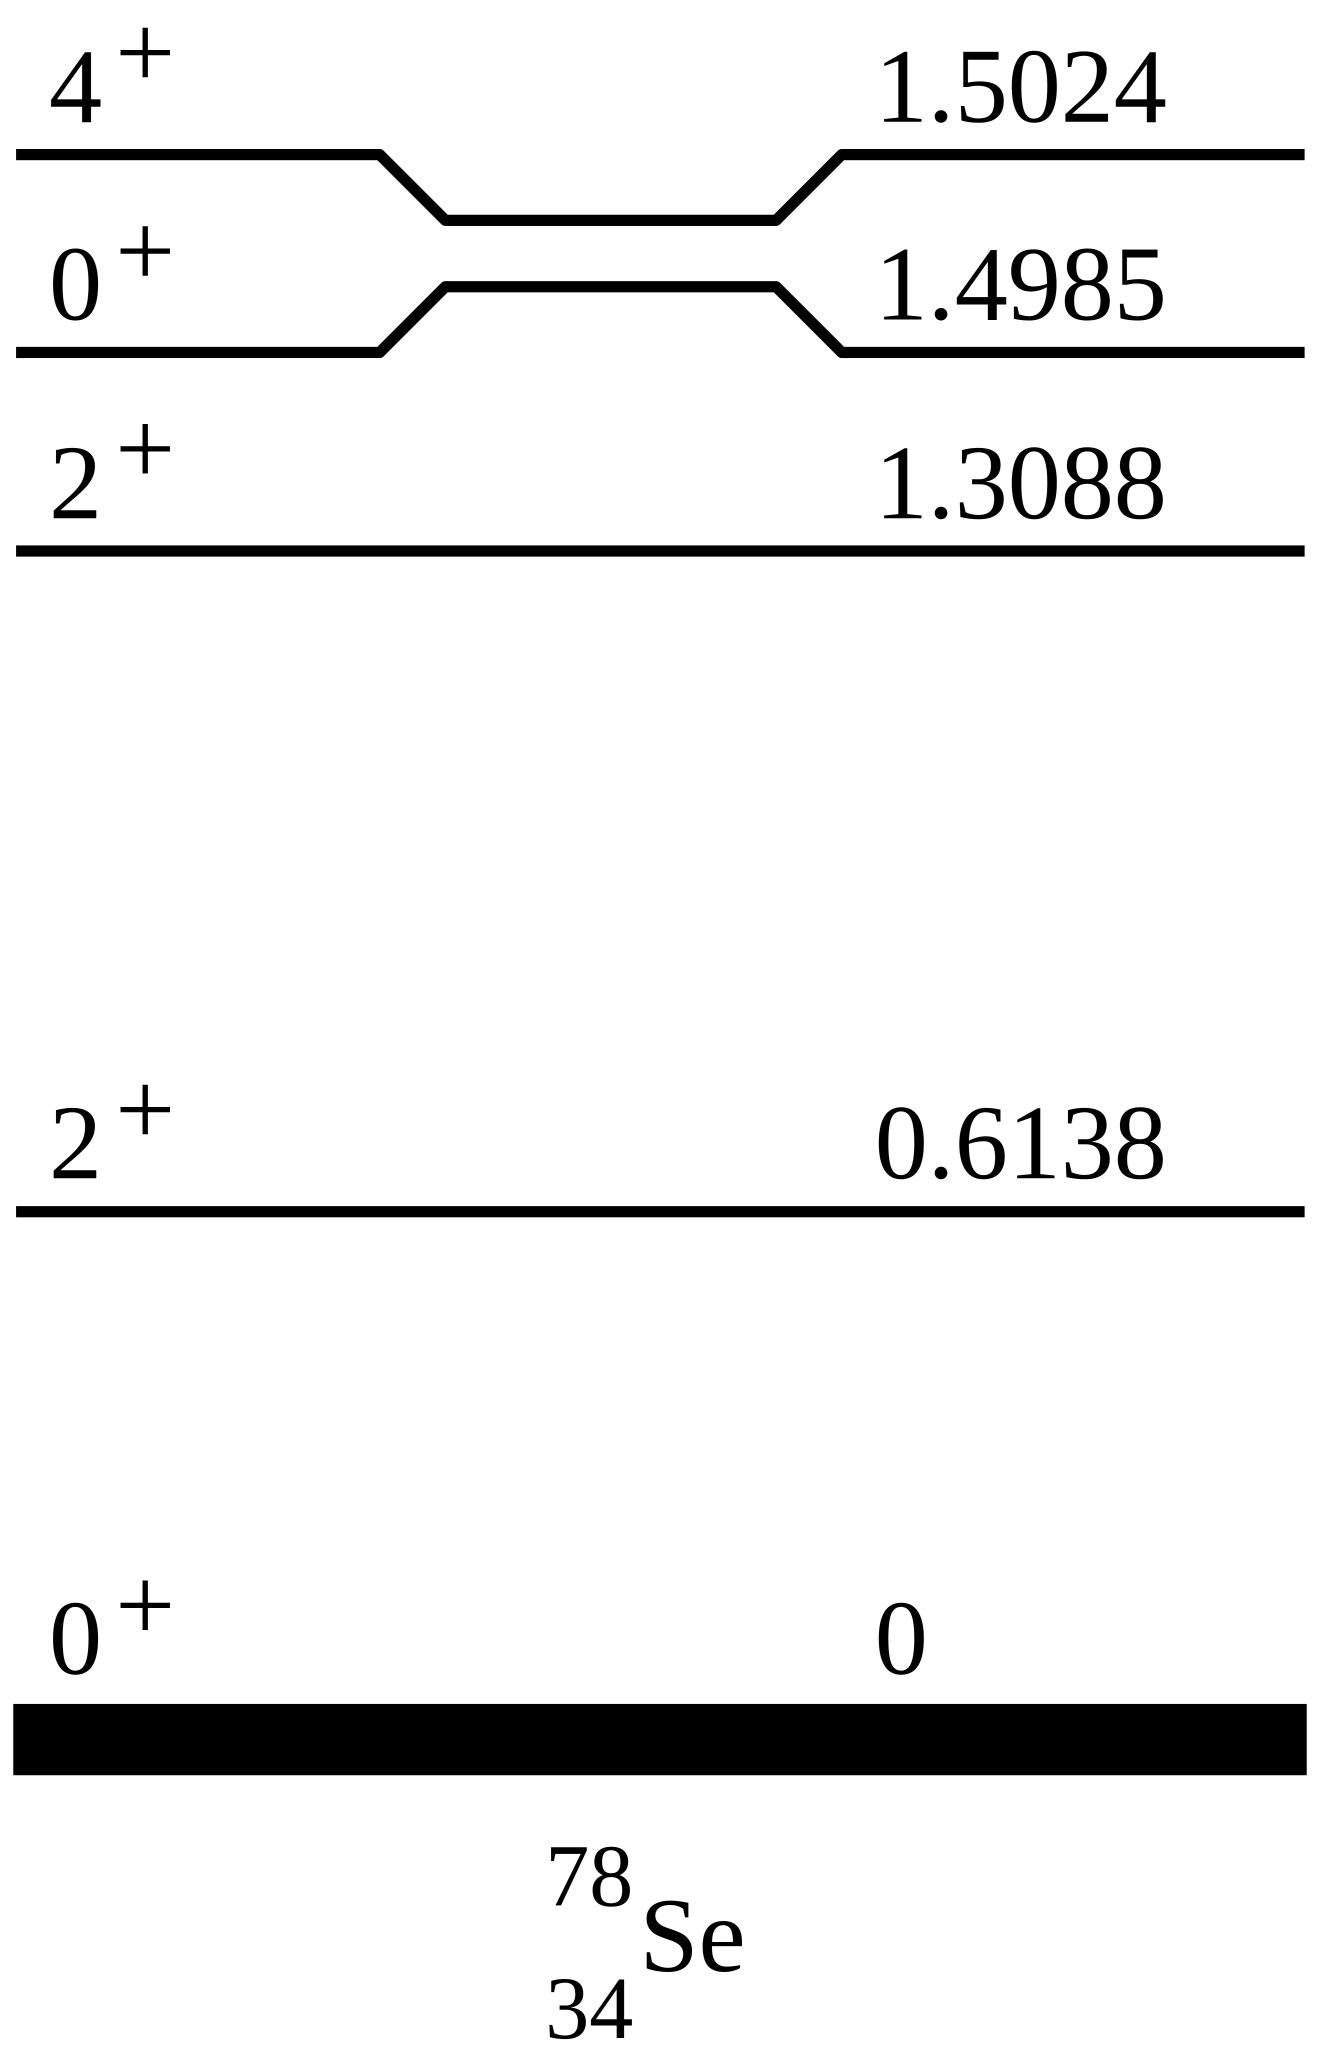
\includegraphics[width=0.3\textwidth]{figures/78Ge_levels.eps}
}
\subfloat[][]{
   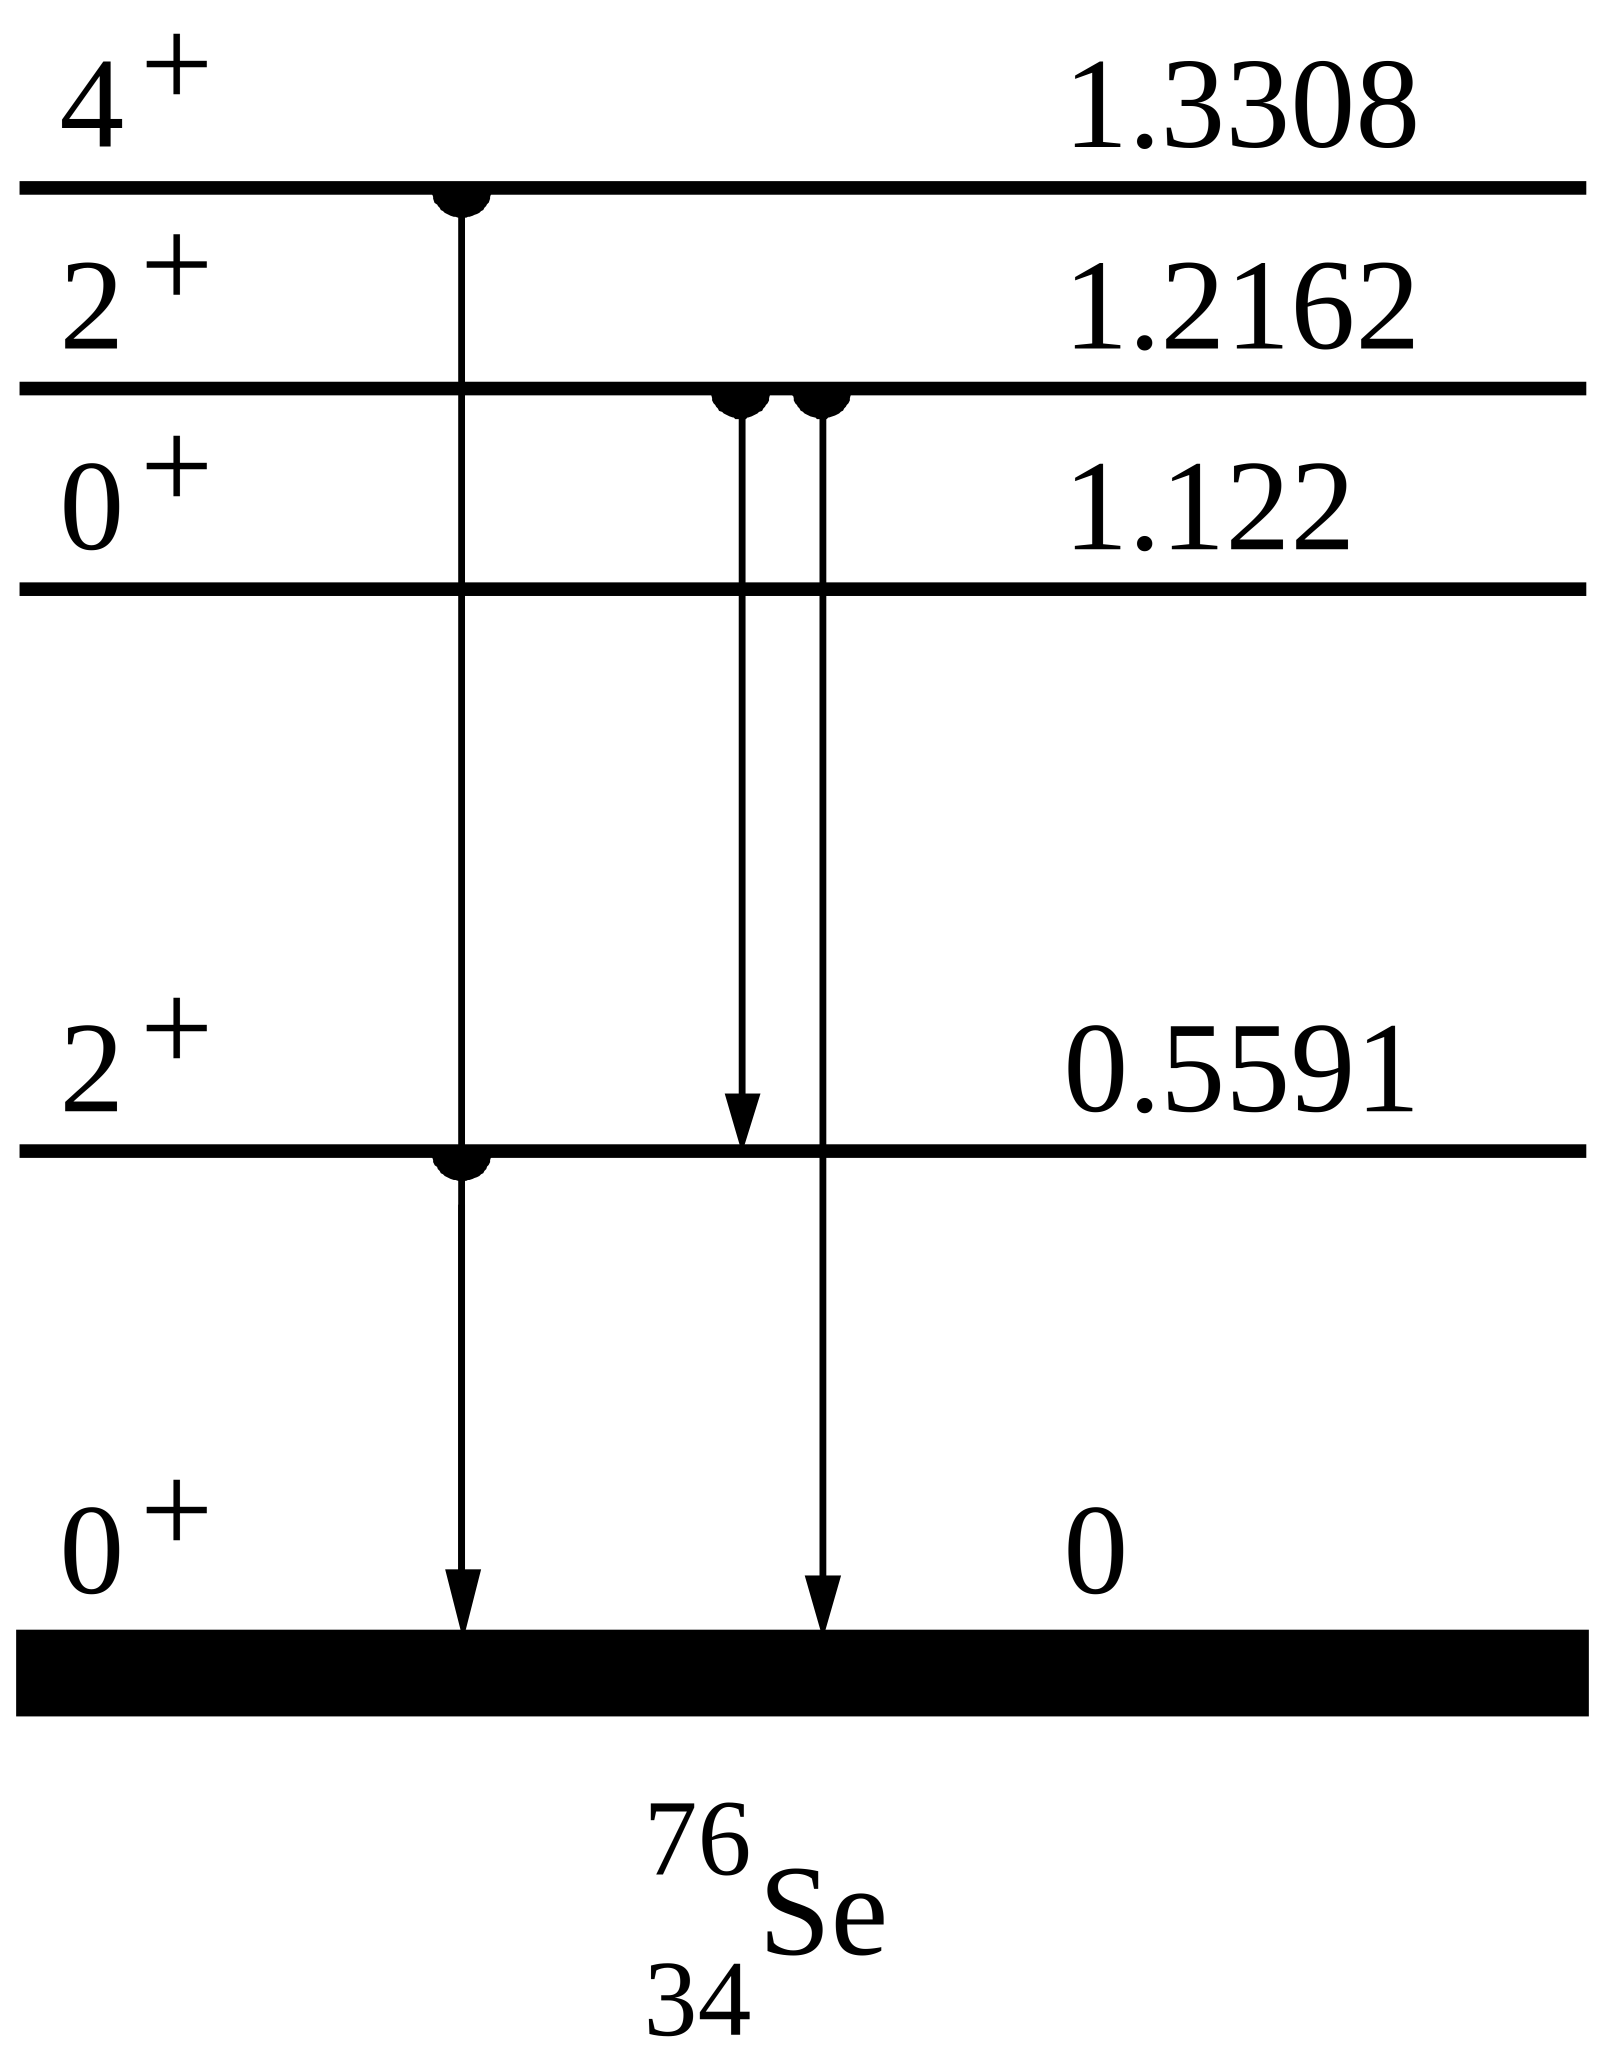
\includegraphics[width=0.3\textwidth]{figures/76Ge_levels.eps}
}
\caption{The level diagrams of the product nuclei, \Se{78} and \Se{76}.  Note the low-lying 2$^+$ state.  Notice also that both nuclei have known \zp levels.  These levels have been measured through $\gamma$-ray experiments.  Such experiments are not sensitive to the pairing in ground-state nuclei, which is why two-nucleon transfer reactions on \zvbb candidate nuclei are of such interest.}
\label{fig:levelDiagrams}
\end{figure}
Particulars of the beam and neutron detector are discussed in {\chap}~\ref{chap:2pExpt} and an analysis of the results in {\chap}~\ref{chap:dataAnalysis}.
% % uncomment the following lines,
% if using chapter-wise bibliography
%
% \bibliographystyle{ndnatbib}
% \bibliography{example}



%
% Chapter 3
%

%
% Modified by Sameer Vijay
% Last Change: Wed Jul 27 2005 13:00 CEST
%
%%%%%%%%%%%%%%%%%%%%%%%%%%%%%%%%%%%%%%%%%%%%%%%%%%%%%%%%%%%%%%%%%%%%%%%%
%
% Sample Notre Dame Thesis/Dissertation
% Using Donald Peterson's ndthesis classfile
%
% Written by Jeff Squyres and Don Peterson
%
% Provided by the Information Technology Committee of
%   the Graduate Student Union
%   http://www.gsu.nd.edu/
%
% Nothing in this document is serious except the format.  :-)
%
% If you have any suggestions, comments, questions, please send e-mail
% to: ndthesis@gsu.nd.edu
%
%%%%%%%%%%%%%%%%%%%%%%%%%%%%%%%%%%%%%%%%%%%%%%%%%%%%%%%%%%%%%%%%%%%%%%%%

%
% Chapter 3
%

\chapter{TWO PROTON TRANSFER AT NOTRE DAME}
\label{chap:2pExpt}

\begin{comment}
Give an overview of the requirements for two-proton transfer and say that ND has a buncher and a Tandem accelerator that goes up to 10 MV so we can get beam energies up to 30 MeV for \He{3} and we have a beamline with a long flight path SO we can do this experiment.
\end{comment}

The previous chapter demonstrated the interest in studying \reaction reactions.  The detected reaction product is a neutron and its time of flight (TOF) must be measured.  The beam must therefore be bunched and the neutron detector must be optimized to provide excellent timing information.  The bunching of the beam and the timing properties of the neutron detector will be discussed in detail in this chapter.   

% detecting neutrons
% this means we need timing information
% so the beam must be bunched
% and the detector must be built to give good timing
% and placed to give good timing

% interested in 0+ distribution
% and there's an ideal beam energy for that
% and that constrains the distance between the target and neutron detector
Not only must the beam be bunched, its energy must also be carefully chosen.  As discussed in the previous chapter, the purpose of this experiment is to measure the distribution of \zp strength.  According to DWBA calculations, achieving the maximum \zp cross-section for \reaction requires a beam energy near 18 MeV, but the resolution of the neutron detector decreases with increasing neutron energy.  The energy chosen for the \He{3} is 16 MeV, and the effect of this energy on the resolution of the neutron detector is discussed in {\sect}~\ref{sec:detector}.


\section{Beam Production at Notre Dame}
\label{sec:beamProduction}

The beam delivered to the target is 16 MeV bunched \He{3}.  In this section, we will follow the beam through its production and acceleration.

The Helium Ion Source (HIS) provides negative \He{3} ions to the accelerator.  A duoplasmatron ion source filled with \He{3} gas uses a discharge across high voltage to convert some of the gas into plasma.  Electrostatic elements extract positive \He{3} ions from the plasma and accelerate them into a canal filled with lithium vapor.  Lithium is crucial for creating negatively charged beam because it donates electrons generously, and a small fraction of the \He{3} becomes negatively ionized after passing through the canal.  A dipole magnet after the ion source removes the carbon, oxygen, and other impurities that contaminate the \He{3} beam.  Movable, thick tungsten slits stop these contaminants and allow beam within a small range of magnetic rigidity (see {\eqn}~\ref{eqn:rigidity} below) to pass through to the accelerator.  Typically, the maximum output of the HIS is $\sim$1~$\mu$A.

The accelerator at Notre Dame is a tandem Van de Graaff accelerator made by High Voltage Engineering Corporation.  Its maximum terminal potential is 10~MV.  Negatively charged beam enters and accelerates toward the positive terminal, located in the center of the machine. A thin carbon foil ($\sim$ 3 $\mu$g/cm$^2$) in the center of the machine strips electrons from the beam.  The now-positive beam accelerates again, away from the positive terminal. In general, the final energy of a particular beam is then

\begin{equation}
E_{\text{beam}} = E_{\text{HIS}} + (1+q)eV_{\text{T}},
\label{eqn:beamEnergy}
\end{equation}
where $V_{\text{T}}$ is the terminal voltage, $E_{\text{HIS}}$ is the energy of the beam exiting the HIS, $q$ is the charge state of the beam after passing through the carbon foil, and $e$ is the charge on the electron.  \He{3} beam is fully stripped of its electrons by the carbon foil, and so the terminal voltage required to produce 16 MeV \He{3} is 5.33~MV, well within the operating voltage range of the accelerator.    

A dipole magnet with a magnetic field strength $B$ will bend a particle with momentum $p$ and charge $qe$ in a circle of radius $R$.  The product of the field strength and the radius of the path, $BR$, is called the magnetic rigidity, and is proportional to the ratio of the momentum and the charge of a particle:

\begin{equation}
BR = \frac{p}{qe} = \frac{\sqrt{2mE}}{qe}.
\label{eqn:rigidity}
\end{equation}

A large 90$^{\circ}$ bend dipole magnet at the exit of the tandem can work in a feed-back circuit to regulate the terminal voltage.  Since the mass and charge of the desired beam are fixed, selecting beam at a fixed radius exiting a dipole defines its energy.  Horizontal slits at the dipole entrance and exit are approximately one millimeter apart.  Both sets of slits serve to narrowly define the beam, but the slits after the analyzing magnet each read the current from incident beam.  This slit current is a sensitive measure of the terminal voltage and is used in a feed-back circuit to maintain a constant beam energy.  Since the radius of the dipole magnet is one meter, the momentum is defined to one part in 1000 and the energy to two parts in 1000 for a fixed magnetic field.  If the terminal voltage drifts up or down, the beam energy will change with it and the beam trajectory will travel a larger or smaller radius through the dipole.  For \He{3}, $E_{\text{beam}}\sim3V_{\text{T}}$, and so a change in the terminal voltage of even one part in 1000 will alter the balance of the slit current.  Because this regulation is limited by the stability of the magnetic field of the dipole, the analyzing magnet is calibrated against the nuclear magnetic resonance (NMR) of hydrogen.  Using it to regulate the terminal voltage reduces the ripple in the voltage to approximately 10~kV.


\subsection{Beam Focusing and Selection}

Beam exiting the analyzing magnet is narrowly defined by horizontal and vertical slits.  Additionally, both pole faces of the analyzing magnet are shaped to provide a focusing field in both the horizontal and vertical planes.  Although the beam has a limited angular divergence at the analyzing magnet, the flight path to the target is $\sim60$~m and and many focusing and steering elements along the way are necessary to obtain a reasonable transmission rate and ensure that the beam is well-focused at the target.  See {\fig}~\ref{fig:beamline} for a schematic diagram of the focusing and steering elements along the beamline.  Two Einzel lenses \citep{BeamOptics} focus the beam before it enters the accelerator, and a set of electrostatic steerers before and after the accelerator are enough to position the beam before it enters the analyzing magnet.  Quadrupole doublet magnets focus the beam as it travels through the target rooms, and another set of steerers allows correction of the beam position and angle.  The final focusing elements before the target are two large-bore, variable-strength solenoid magnets \citep{TwinSol} that focus the beam to a spot approximately 2~mm in diameter.

% figure: beamline
\begin{figure}[htp]
\centering
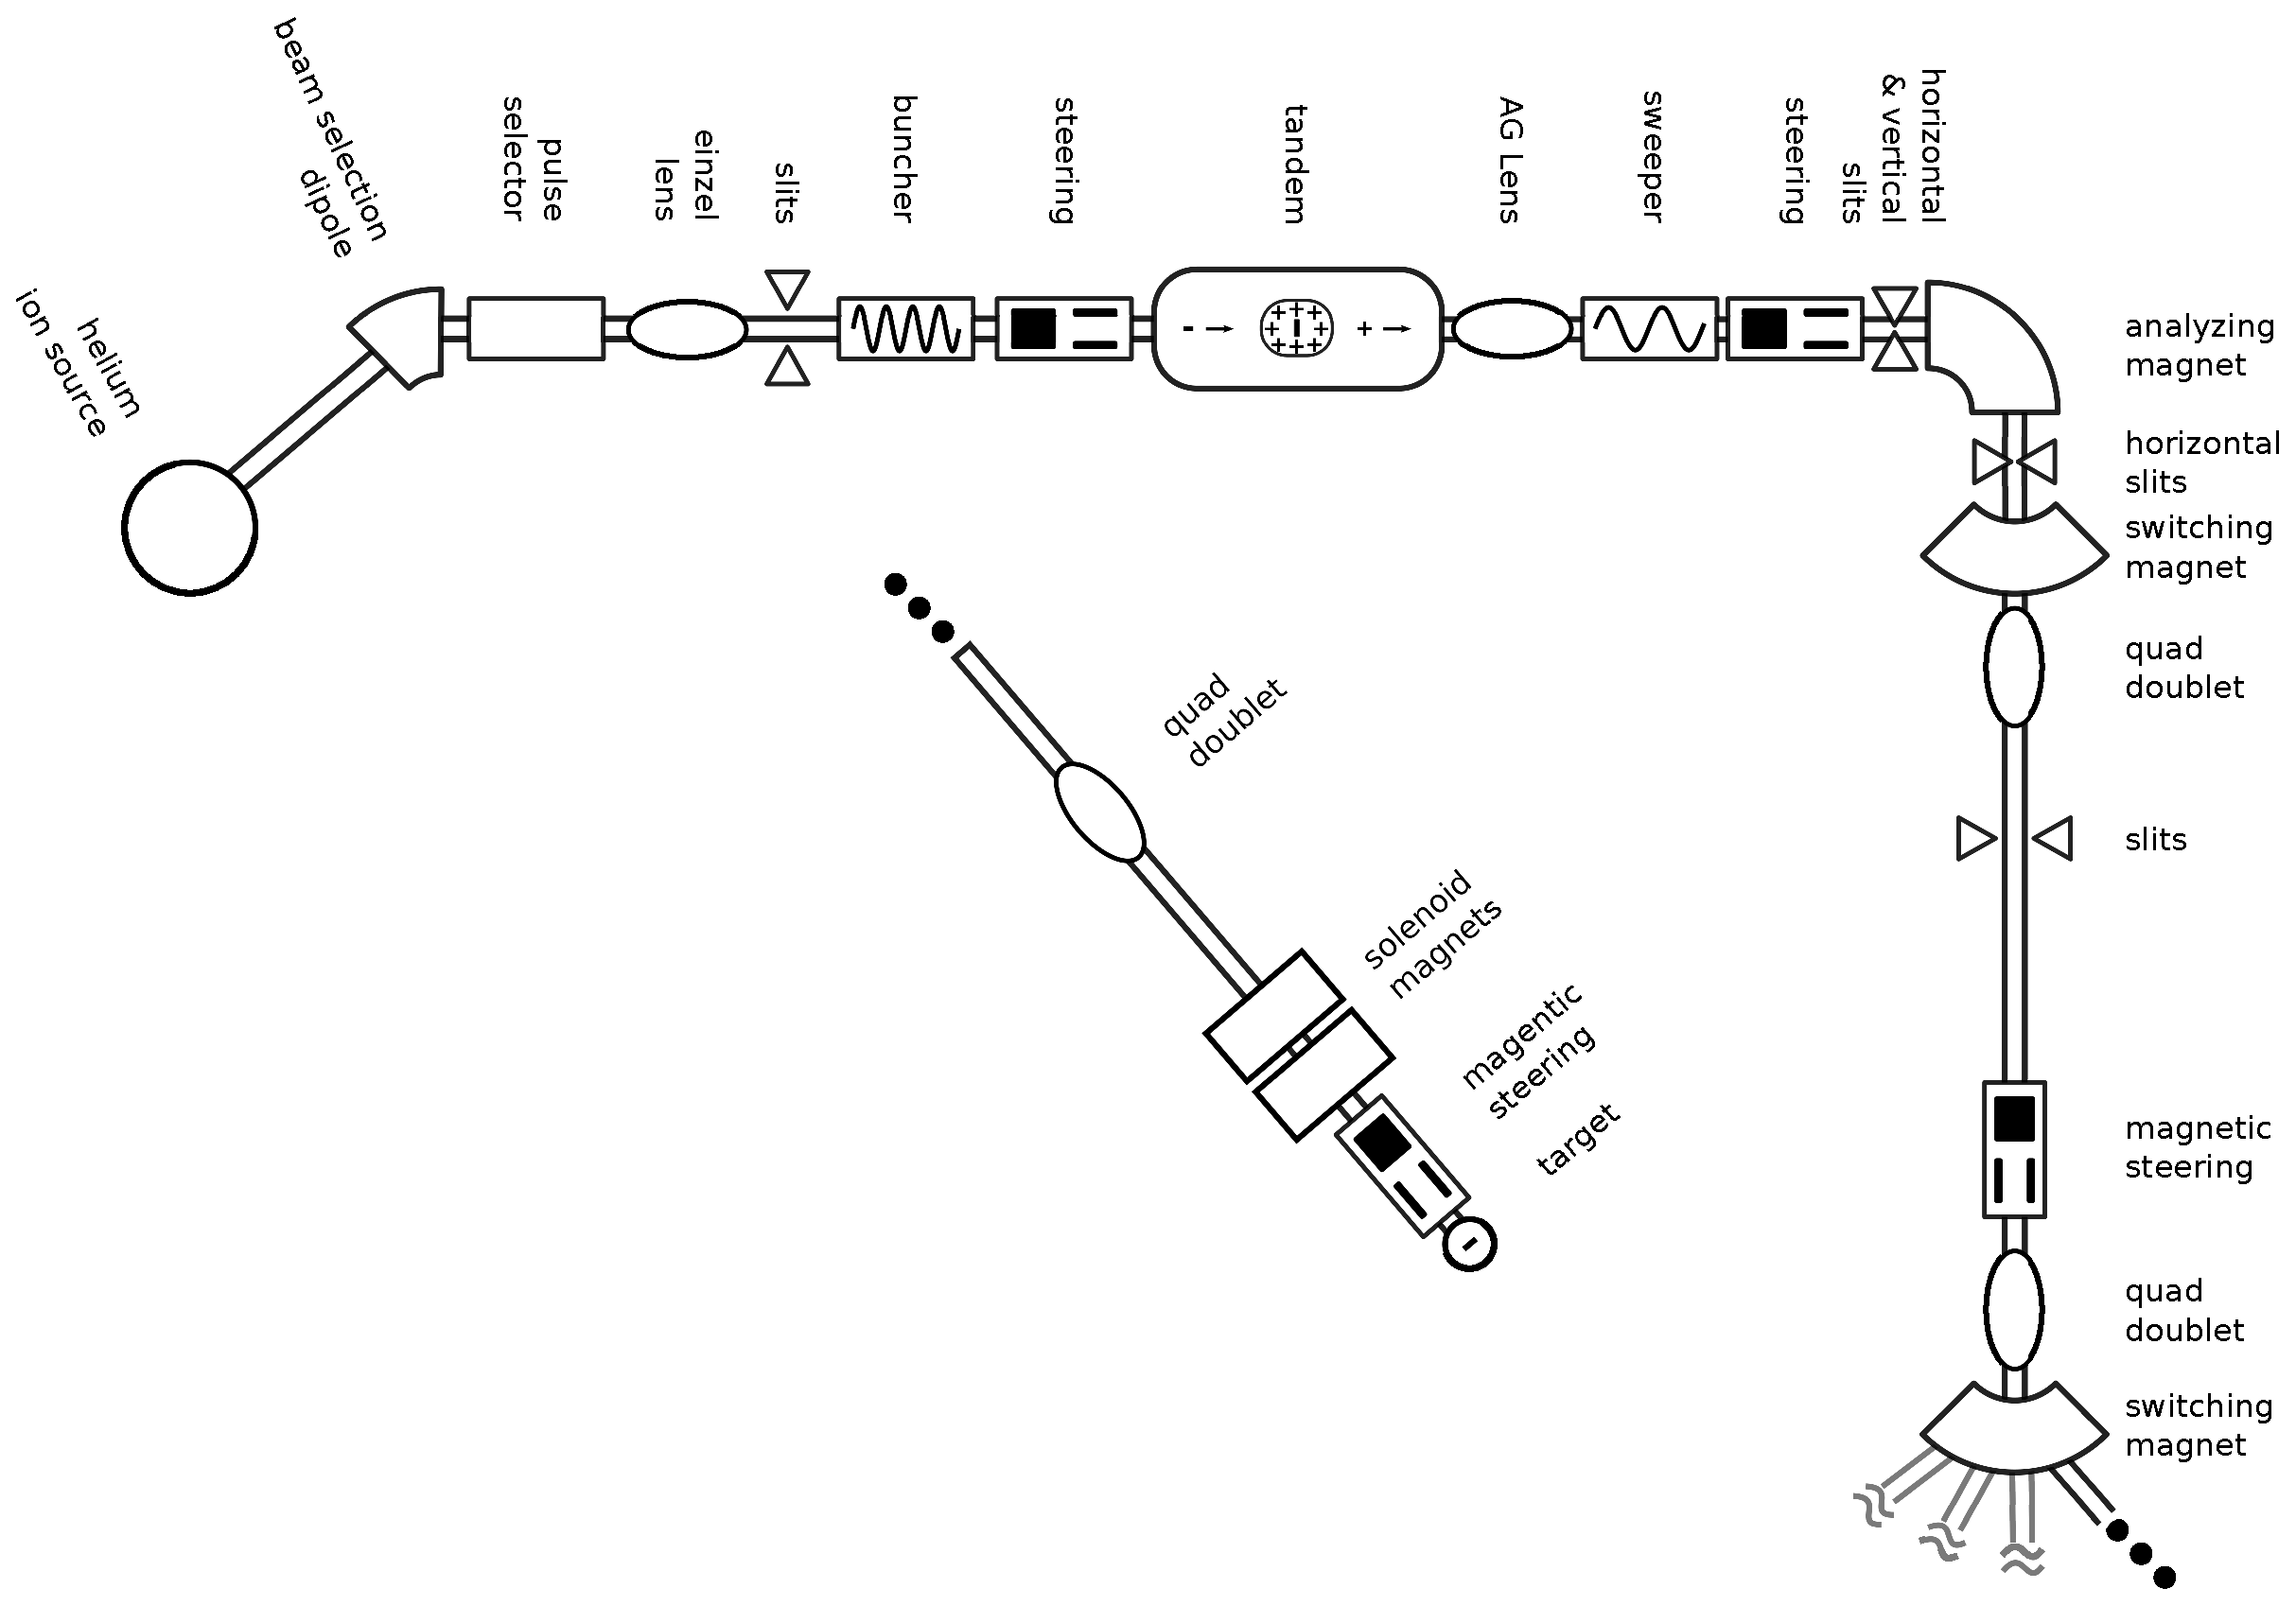
\includegraphics[width=1.0\textwidth]{figures/NSL_beamline.eps}
\caption[Beam production at Notre Dame.]{Beam production at Notre Dame.  The center inset shows the 15$^{\circ}$ beamline that was used in the experiments.}
\label{fig:beamline}
\end{figure}

\subsection{Beam Bunching}

Continuous beam would make it impossible for our detector to determine the neutron TOF.  It is possible to bunch the beam so that ``bunches'' of \He{3} arrive at the target, each bunch having a time spread of approximately one ns. There are three components to the bunching system at Notre Dame.  The first is the buncher itself, which pushes about 40\% of the beam into discrete bunches.  The remaining 60\% is a continuous background and must be removed with the ``sweeper''.  Together, the buncher and sweeper provide bunches of beam that are 1 ns wide at the target and separated by 101 ns, with no beam in between.  With the detector approximately 15 m away from the target, some of the slow neutrons coming from the reaction have a TOF in excess of 300 ns.  A pulse-selector is used to eliminate three out of every four bunches to avoid overlapping energetic neutrons from the current beam bunch with slow neutrons from the previous bunch.  The buncher, sweeper, and pulse-selector together provide clean bunches of beam separated by 400 ns.  The rest of this section describes how each of these components works.

The beam buncher operates by slowing down particles that would arrive too early at the target and speeding up particles that would be arriving too late.  To achieve this, two grids perpendicular to the beam connect to a radio-frequency (RF) power supply to create a time-varying electric field.  If the electric field were a sawtooth wave in time, the beam bunches would contain all the beam \citep{LynchBunching}.  As illustrated in {\fig}~\ref{fig:bunching}, the buncher decelerates the early portion of the beam and accelerates the late portion of the beam.  The strength of the field determines the distance at which the bunch will be narrowest, with a stronger field bringing the bunch into time focus earlier than a weaker field.  The pure sawtooth field is able to bunch 100\% of the incoming beam because it immediately resets after its linear portion.  Commercially available RF power supplies, however, generally vary sinusoidally in time.  At Notre Dame, a single frequency buncher that operates at 9.85 MHz is used.  While the RF signal is increasing approximately linearly with time, beam is bunched exactly as if the field were a pure sawtooth wave.  When the electric field approaches a maximum or minimum, little bunching occurs, and when the electric field is decreasing, de-bunching occurs.  The sinusoidal RF supply results in nanosecond wide bunches containing $\sim$40\% of the beam arriving at the target every 101~ns, superimposed on a continuous background of the remaining beam.  This continuous beam would render our time signal useless and must somehow be removed.

% figure: how a beam buncher works
\begin{figure}[htp]
\centering
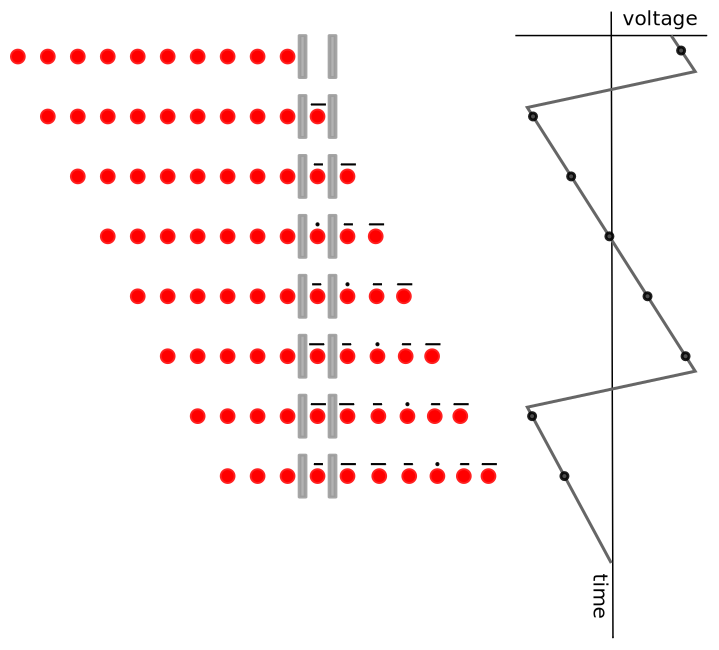
\includegraphics[width=1.0\textwidth]{figures/beamBunching.eps}
\caption[Beam bunching.]{Beam bunching using a time-varying electric field.  Each dot represents a beam particle, and the vertical gray bars represent the bunching electrodes.  To bunch one section of beam, particles arriving first must be slowed down, while particles arriving last must be sped up.  A linearly increasing field does exactly this.  If the wave is a perfect sawtooth, there is no time during which beam is not being bunched - that is, all the beam is bunched.  Notice also that beam does not exit the buncher in a tight bunch; as time passes, beam drifts together.  The time until the bunch is at its narrowest depends on the amplitude of the electric field applied by the buncher.}
\label{fig:bunching}
\end{figure}

The ``sweeper'' provides a sinusoidal electric field that is timed to deflect the continuous beam between the bunches.  A set of vertical slits immediately after the sweeper removes the deflected beam.  Variable delays allow adjustment of the timing between the buncher and the sweeper and must be optimized for a particular beam.  Even a few-nanosecond change in the timing can affect which portion of the beam is swept away. 

%figure of beam profile and sweeper

It is possible to take data without pulse selection.  However, the spread in TOF of the neutron spectrum is in excess of 300~ns, which complicates the TOF spectrum considerably.  With bunches arriving at the target every 101~ns, it will be impossible to tell if a neutron is very fast and associated with the current bunch or very slow and associated with the previous bunch.  The resulting spectrum is shown in Figure \ref{fig:PSvsNPS_TOF}.

% figure: the considerably complicated spectrum
\begin{figure}[htp]
\centering
\subfloat[][]{
   \includegraphics[width=0.45\textwidth]{figures/PS_BarA_Sep.eps}	
}
\subfloat[][]{
	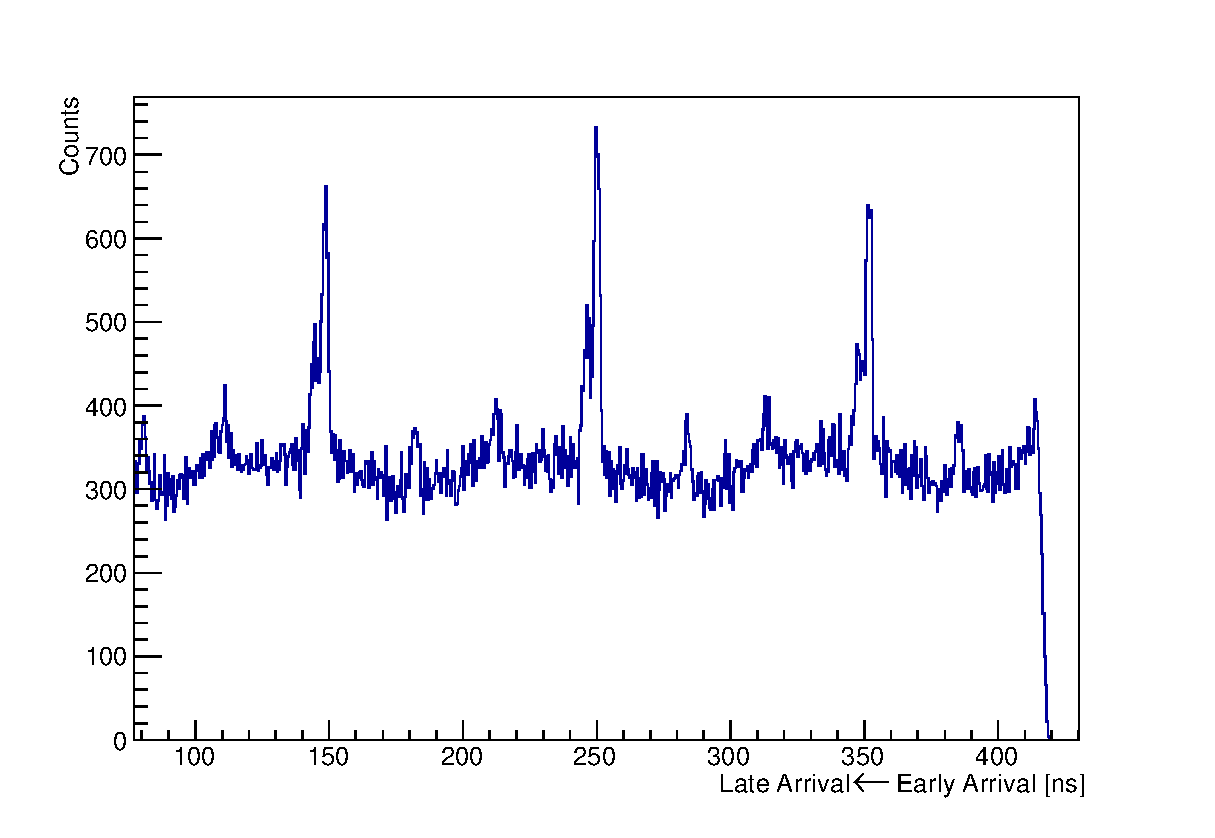
\includegraphics[width=0.45\textwidth]{figures/NPS_BarA.eps}
}
\caption[Timing spectra due to pulse-selected and non-pulse-selected beam.]{The timing spectrum from a pulse-selected beam is shown in (a).  The timing spectrum in (b) is from beam with no pulse selection.  Both timing spectra are from a \He{3} beam on a \Ge{76} target.  The constant background present in both images is due to random background radiation, not the beam.}
\label{fig:PSvsNPS_TOF}
\end{figure}

To give all the neutrons resulting from one beam bunch time to reach the detector before the next bunch strikes, a ``pulse selector'' eliminates three of every four bunches, resulting in 404~ns between each bunch at the cost of beam intensity.  The pulse selector is located before the accelerator and consists of two parallel plates, one held at ground and the other at +400 V.  A fast switch (SCR) connects the high-voltage plate to ground, letting the selected bunch through without deflection.  Vertical slits immediately after the pulse selector remove deflected beam, while undeflected beam passes through to the accelerator.  While the beam width is only one ns at the target, at the sweeper the bunch is approximately 80~ns wide, so the SCR must hold the plate at ground for 80~ns to let the entire bunch through.
% figure: slow neutrons and their dissappearance

Beam bunching and pulse selection reduce available beam current - the swept beam current is only 40\% $\times$ $\frac{1}{4} = 10$\% of the non-bunched current.  However, without bunched beam it would not be possible to distinguish the neutrons of interest in the (\He{3},n) transfer reaction.  Increased beam current would improve statistics on \reaction, but the HIS was already operating at its full output for these experiments.

\section{The Target Chamber}
\begin{comment}
target
thin stainless steel wall
Si detector
BaF$_2$ detector
\end{comment}

The 16 MeV \He{3} beam has been bunched, swept, pulse-selected, and steered and focused onto the target.  The bunches that were 80~ns wide before the accelerator have converged into 1-ns wide bunches at the target.  The target is at the center of a 2-mm thick stainless steel chamber that has a small gold-lined Faraday cup as shown in {\fig}~\ref{fig:targetChamber}.

To measure the absolute scale of the cross-section, it is necessary to know the number of particles incident on the target.  The charge measured by the Faraday cup is directly proportional to this number.  Additional detectors sensitive to the product of the beam current and the target thickness monitor the beam and provide relative normalization.  One of these is a Si detector placed inside the target chamber, which monitors \He{3} beam scattered from the target.  The other monitor detector is a BaF$_2$ detector located just outside the chamber.  It is sensitive to $\gamma$ radiation produced by beam interactions in the target.  
% figure: the target chamber & its detectors
\begin{figure}[htp]
\centering
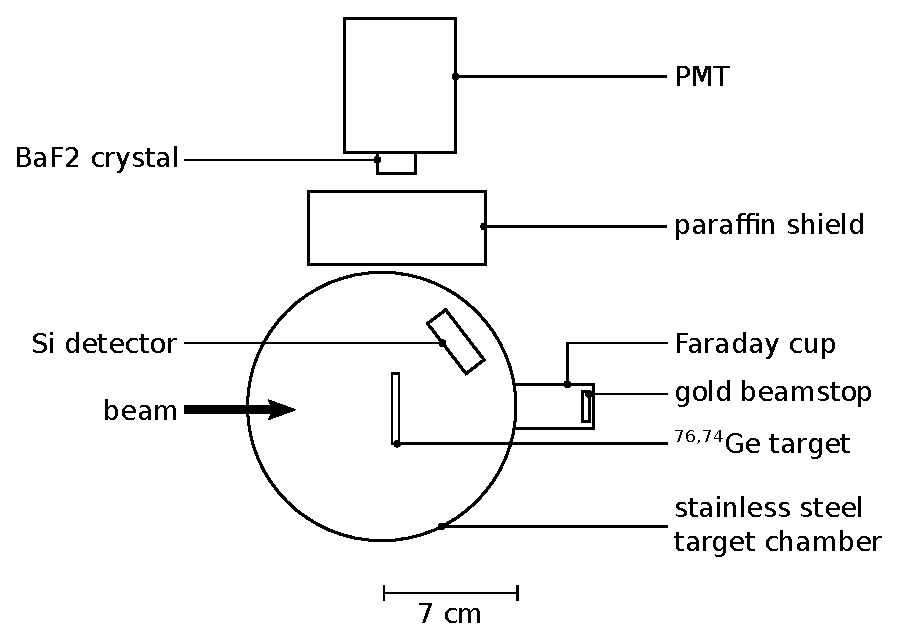
\includegraphics[width=1.0\textwidth]{figures/targetChamber.eps}
\caption[The target chamber and beam monitors.]{The target chamber and beam monitors.  The Si detector detects scattered \He{3} ions while the BaF$_2$ crystal primarily detects $\gamma$ radiation from the target.  Note that a paraffin block shields the BaF$_2$ detector from neutron radiation, which also escapes the target chamber.}
\label{fig:targetChamber}
\end{figure}


\section{The Neutron Detector}
\label{sec:detector}
\begin{comment}
Discuss neutron wall briefly.  Can reference NIMA paper. Explain why it's important that it's wide-angle. 
\end{comment}

The products of two-proton transfer onto \GeTargets are a neutron and a \SeProducts nucleus.  The neutron, lacking charge, is not likely to interact with remaining material in the target and has only a $\sim$5\% chance of scattering from the stainless steel target chamber.  This low rate of interaction, however, poses a challenge when the goal is to detect the neutron.  The neutron detector at Notre Dame maximizes the chance of a neutron interaction by providing protons with which the neutrons can strongly interact.  Unlike charged particles, neutrons rarely deposit their full energy in a detector.  Neutrons can only deposit all their energy when they collide head-on with a proton.  Much more likely is a glancing interaction, where the neutron imparts only some of its energy to the proton.  The measured energy spectrum of monoenergetic neutrons ranges from the detector threshold up to the neutron's full energy, making it impossible to determine the energy of the neutron from its deposited energy.  Instead, the time of flight (TOF) between the target and the detector is used to distinguish neutrons of differing energies.  The neutron detector is optimized to provide precise timing information.       
% figure of charged-particle energy spectrum
% figure of neutron energy spectrum

The neutron detector \citep{KolataNeutwall} consists of 16 large (1.5 m $\times$ 0.15 m $\times$ 0.05 m) bars of commercially available scintillator with excellent timing response \citep{BC408}.  Each plastic scintillator bar is equipped with two fast-risetime photomultiplier tubes (PMT's) at opposite ends.  The signal risetimes are approximately 5~ns, and by processing the signal with constant fraction discriminators (CFD's) the timing resolution of the PMT's is sub-nanosecond.  Additionally, PMT's on opposite ends of the bars allows construction of an average time signal, removing the timing spread due to the interaction location.  Neutron detector signal processing is discussed further in {\sect}~\ref{sec:electronics}.
% figure: one bar with its PMT's

% table: BC408 properties
\begin{table}[htp]
\centering
\caption[\uppercase{plastic scintillator properties}]{\uppercase{plastic scintillator properties}}
\label{tab:BC408}
\begin{tabular}{ll}
Properties & BC408 \\
\hline
Light Output, \% Anthracene & 64 \\
Rise Time, ns & 0.9 \\
Decay Time, ns & 2.1 \\
Pulse Width, FWHM, ns & $\sim2.5$ \\
Light Attenuation Length, cm & 210 \\
Wavelength of Max. Emission, nm & 425 \\
No. of H Atoms per cm$^3$ & 5.23$\times10^{22}$ \\
No. of C Atoms per cm$^3$ & 4.74$\times10^{22}$ \\
Ratio H:C Atoms & 1.104 \\
No. of Electrons per cm$^3$ & 3.37$\times10^{22}$ \\
\end{tabular}
\begin{flushleft}
\small NOTE:
Properties of the plastic scintillator used as the neutron detector. Values are taken from \citep{BC408}.
\end{flushleft}
\end{table}

The bars of scintillating plastic are positioned on an arc of radius 14.6 m centered around the target as shown in {\fig}~\ref{fig:detectorGeometry}.   At this distance, the solid angle subtended by each bar is only 0.15 m/15 m $\times$ 1.5 m/15 m = 1 msr.  The forwardmost angle relative to the beam is 6$^{\circ}$ and the largest angle is $22^{\circ}$.  As discussed in the previous chapter, the angular distribution of the \zp states peaks at 0$^{\circ}$ and drops to its first minimum at 20$^{\circ}$, so that ideally the detector would extend to 0$^{\circ}$.  A concrete support beam makes 6$^{\circ}$ the forwardmost instrumentable angle.
% figure - diagram of detector
\floatsetup[figure]{style=plain,subcapbesideposition=top}
\begin{figure}[htp]
\centering
\sidesubfloat[][]{
   \includegraphics[width=1.0\textwidth]{figures/detectorLayout.eps}
}
\qquad
\sidesubfloat[][]{  
   \includegraphics[width=0.35\textwidth]{figures/neutDetector_groupOfFour_crop.eps}
}
\caption[A schematic of the neutron detector and its supporting structure.]{A schematic of the neutron detector is shown in (a).  The figure is not to scale.  The detector is comprised of 16 independent scintillating bars, grouped in fours on separate support structures.  One of the supports is shown in (b).  Each individual bar of scintillator has a PMT fastened to its top and bottom surface.}
\label{fig:detectorGeometry}
\end{figure}

The 14.6~m flight path was not arbitrarily chosen; the distance between the target and detector must be as long as possible to ensure reasonable resolution.  The longest available path in the room was $\sim$15~m.  Together with the neutron energy, this distance determines the resolution of the detector.  Conservation of energy and momentum determines the relativistic energy $E = \gamma m c^2$ of the outgoing neutron, where $\gamma=(1-v^2/c^2)^{-1/2}$ and $m$ and $v$ are the rest mass and velocity of the neutron, respectively.  The time $t$ it takes for this neutron to travel the distance $d$ between the target and the detector is fixed for a given $d$ and $v$.  Deriving this time as a function of the relativistic energy is simple using the relation $E=\gamma mc^2$, where $c$ is the speed of light:
\begin{equation}
t(E) = \frac{d}{v} =  dc\times\sqrt{\frac{(E/mc^2)^2}{(E/mc^2)^2-1}} 
\label{eq:TOF}
\end{equation}
Neutrons from $^{76}$Ge($^3$He,n)$^{78}$Se have a relativistic energy of $\sim$966~MeV if the product nucleus, $^{78}$Se, is populated in its ground state.  Using {\eqn}~\ref{eq:TOF}, this gives a TOF of
\begin{eqnarray}
t(966 \text{ MeV}) &=& (14.6 \text{ m})(0.3 \text{ m/ns})\times\sqrt{\frac{(966/940)^2-1}{(966/940)^2}} \nonumber \\
           &=& (14.6 \text{ m})(0.3 \text{ m/ns})\times\frac{1}{0.23} = 212 \text{ ns} \nonumber.
\end{eqnarray}
Neutrons from a reaction that populates the first excited state of \Se{78}, which is only 0.6~MeV above the ground state, trail the ground-state neutrons by 1.9~ns.  Since the beam bunch itself has a width of 1~ns, this flight path provides not quite enough resolution to separate the ground and first excited state of \GeTargets. However, the differing angular distributions of the two states allowed for a determination of their respective intensities.  This is discussed in {\chap}~\ref{chap:dataAnalysis}.
% figure: \Ge{76}, 74Ge level scheme?


\subsection{Electronics}
\label{sec:electronics}
\begin{comment}
Electronics diagram!  Discuss two most important aspects: TDC and ADC from phototubes
\end{comment}

In principle, the timing information is all the data acquisition (DAQ) needs to record if there were no background radiation.  However, concrete in the room emits low-energy $\gamma$ radiation that leaves signals in the detector at a high rate.  Measuring the energy deposition is necessary because it allows us to eliminate this low-energy background radiation as well as high-energy cosmic rays.

When a particle deposits energy in some bar of the neutron detector, the DAQ must record both the total energy and timing of the signals from the top and bottom PMT's.  A charge to digital converter (QDC) can integrate the PMT signal and a time to digital converter (TDC) can measure the time between a logic pulse created by the PMT signal and the logic pulse from the beam buncher.  Because time resolution is the only way to distinguish groups of neutrons with different energies, constant fraction discriminators (CFD's) and not leading edge discriminators create the logic pulse sent to the TDC.  The 5-ns PMT signal risetime, together with CFD's, give timing information with jitter that is about 1~ns.  There are no stringent requirements on energy resolution as the detector itself has energy resolution on the order of 1~MeV near the thorium edge.
% figure: CFD operation

The lone signal provided by the PMT base is not adequate for pulse processing because the QDC and TDC require separate signals.  The signal from the PMT base is also too small to trigger the CFD's.  A 10$\times$ amplifier makes the signal large enough to trigger the CFD's and provides two copies of the input signal, one which can be analyzed for timing information while the other is analyzed for energy information.  A simplified diagram of the data acquisition is shown in {\fig}~\ref{fig:simpleElectronics}.

% figure: simple electronics
\begin{figure}[htp]
\centering
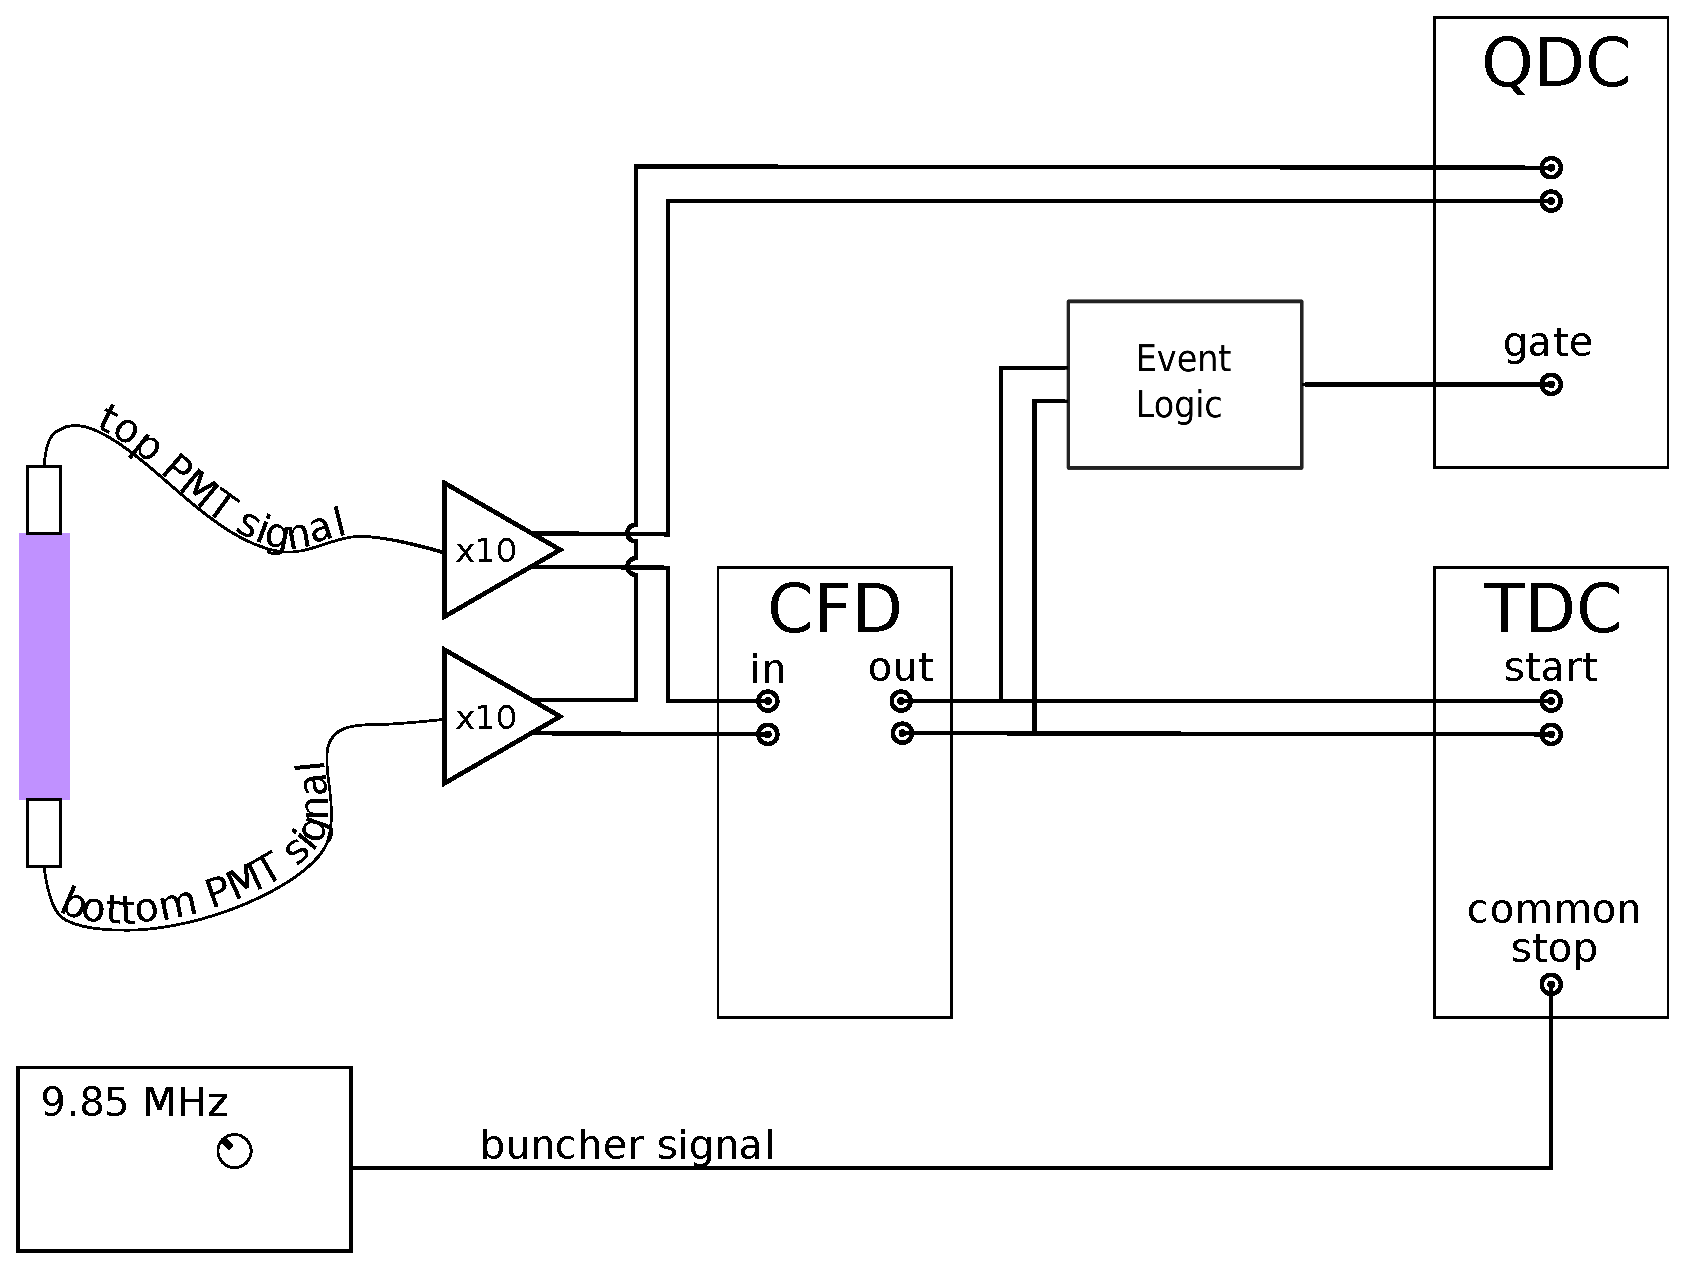
\includegraphics[width=1.0\textwidth]{figures/basic_electronics.eps}
\caption[Simplified sketch of the detector electronics.]{A simplified diagram of the neutron detector electronics showing the acquisition of timing and energy information from a single bar of the detector.}
\label{fig:simpleElectronics}
\end{figure}

The fundamental components of the DAQ are the TDC, the QDC, and the event trigger that causes the DAQ to read each module.  Triggering any time either a bar's top or bottom PMT fired would waste the DAQ with recording many noise events.  A real event should create signals in both the top and bottom PMT's, and requiring a coincidence between the two results is a reasonable trigger.  One way to define an event trigger for the entire neutron wall would be to trigger any time a coincidence between associated top and bottom PMT's occurs.  But constructing this trigger with NIM logic units requires many separate logic gates and is unnecessarily complicated.  

One solution is to use the built-in OR of the CFD.  Each CFD is an eight-fold unit that provides an OR output.  Instead of requiring a top and bottom signal in the same bar, each CFD unit processes a section of only top or only bottom bar signals and the condition is loosened to requiring a signal in a top PMT and a bottom PMT in the same eight-bar group as shown in {\fig}~\ref{fig:eventTrig}.  The presence of some top signal AND some bottom signal triggers the event signal.  Such an event only requires that both a top and a bottom signal coincided but does not require that these signals belonged to the same bar.  This simplified event trigger includes all events of interest, where the top and bottom signal belong to one bar, but also includes spurious events where no bar has a signal in both its top and bottom PMT.  With a dead time of less than 30\%, this event condition does not hinder data collection.  Simple software cuts eliminate any spurious events where no bar has a signal in both its top and bottom PMT.

% figure: event trigger
\begin{figure}[htp]
\centering
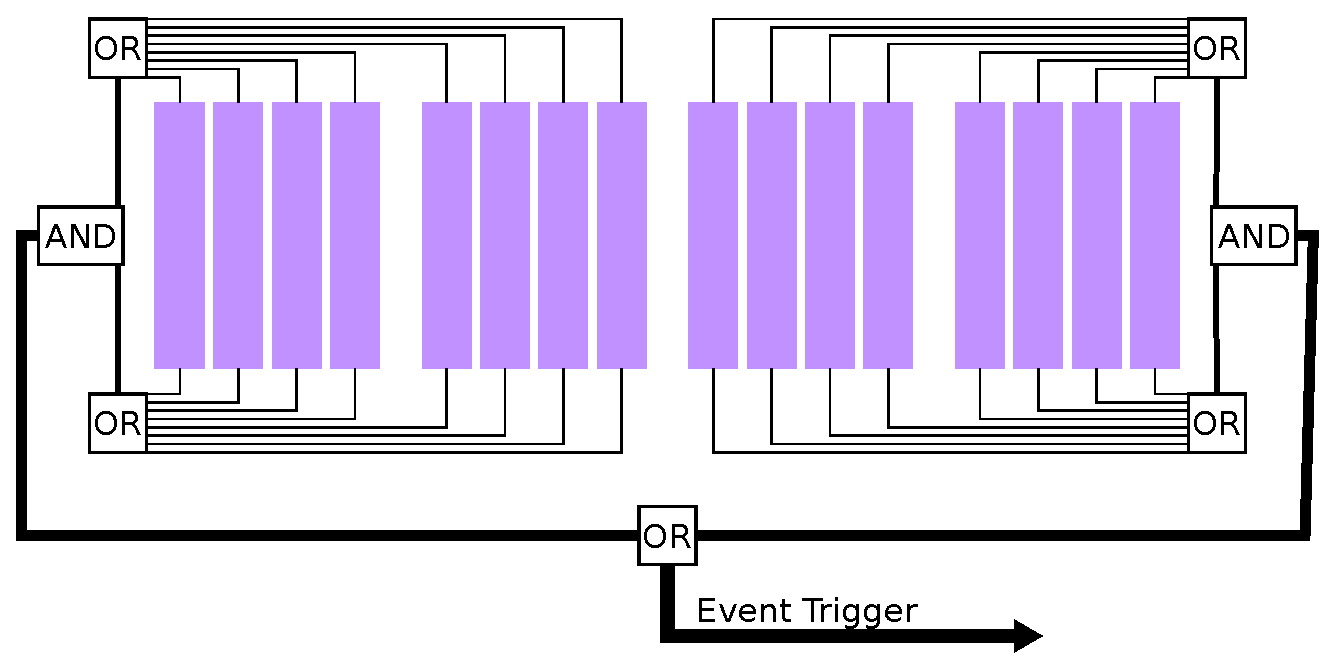
\includegraphics[width=1.0\textwidth]{figures/event_trigger.eps}
\caption[DAQ event trigger.]{The event trigger for the DAQ requires a coincidence between a top PMT and a bottom PMT from the same group of eight bars.}
\label{fig:eventTrig}
\end{figure}

% discuss energy, time info from near-target detectors
% and then scalers?
The time information, energy information, and a signal to indicate that this information should be read from the modules and recorded, form the core of the neutron detector DAQ.  However, the DAQ must also record information from the detectors near the target.  The particles of interest for the Si detector are scattered \He{3} beam, and because they are charged and deposit all their energy in the Si detector, the energy is a useful way to identify scattered \He{3} and should be recorded.  The BaF$_2$ detector sits outside the target chamber and monitors primarily beam-induced $\gamma$ radiation.  The timing of this detector's signal relative to the beam buncher, rather than the energy, is recorded by the DAQ.  Finally, because these detectors have high detection efficiency and are placed close to the target, their event rate is much higher than that of the neutron detectors.  While these detectors are essential to determining the relative particle flux through the target, the dead time they cause the DAQ should not prohibit events from the neutron detector itself from being recorded.  Pre-scaling the signals from the Si and BaF$_2$ by factors of 100 and 50, respectively, before adding it to the event trigger limits the dead time of the total system to less than 20\%.  See {\fig}~\ref{fig:fullElectronics} for a schematic of the complete electronics setup.
% figure: full electronics
\begin{figure}[htp]
\centering
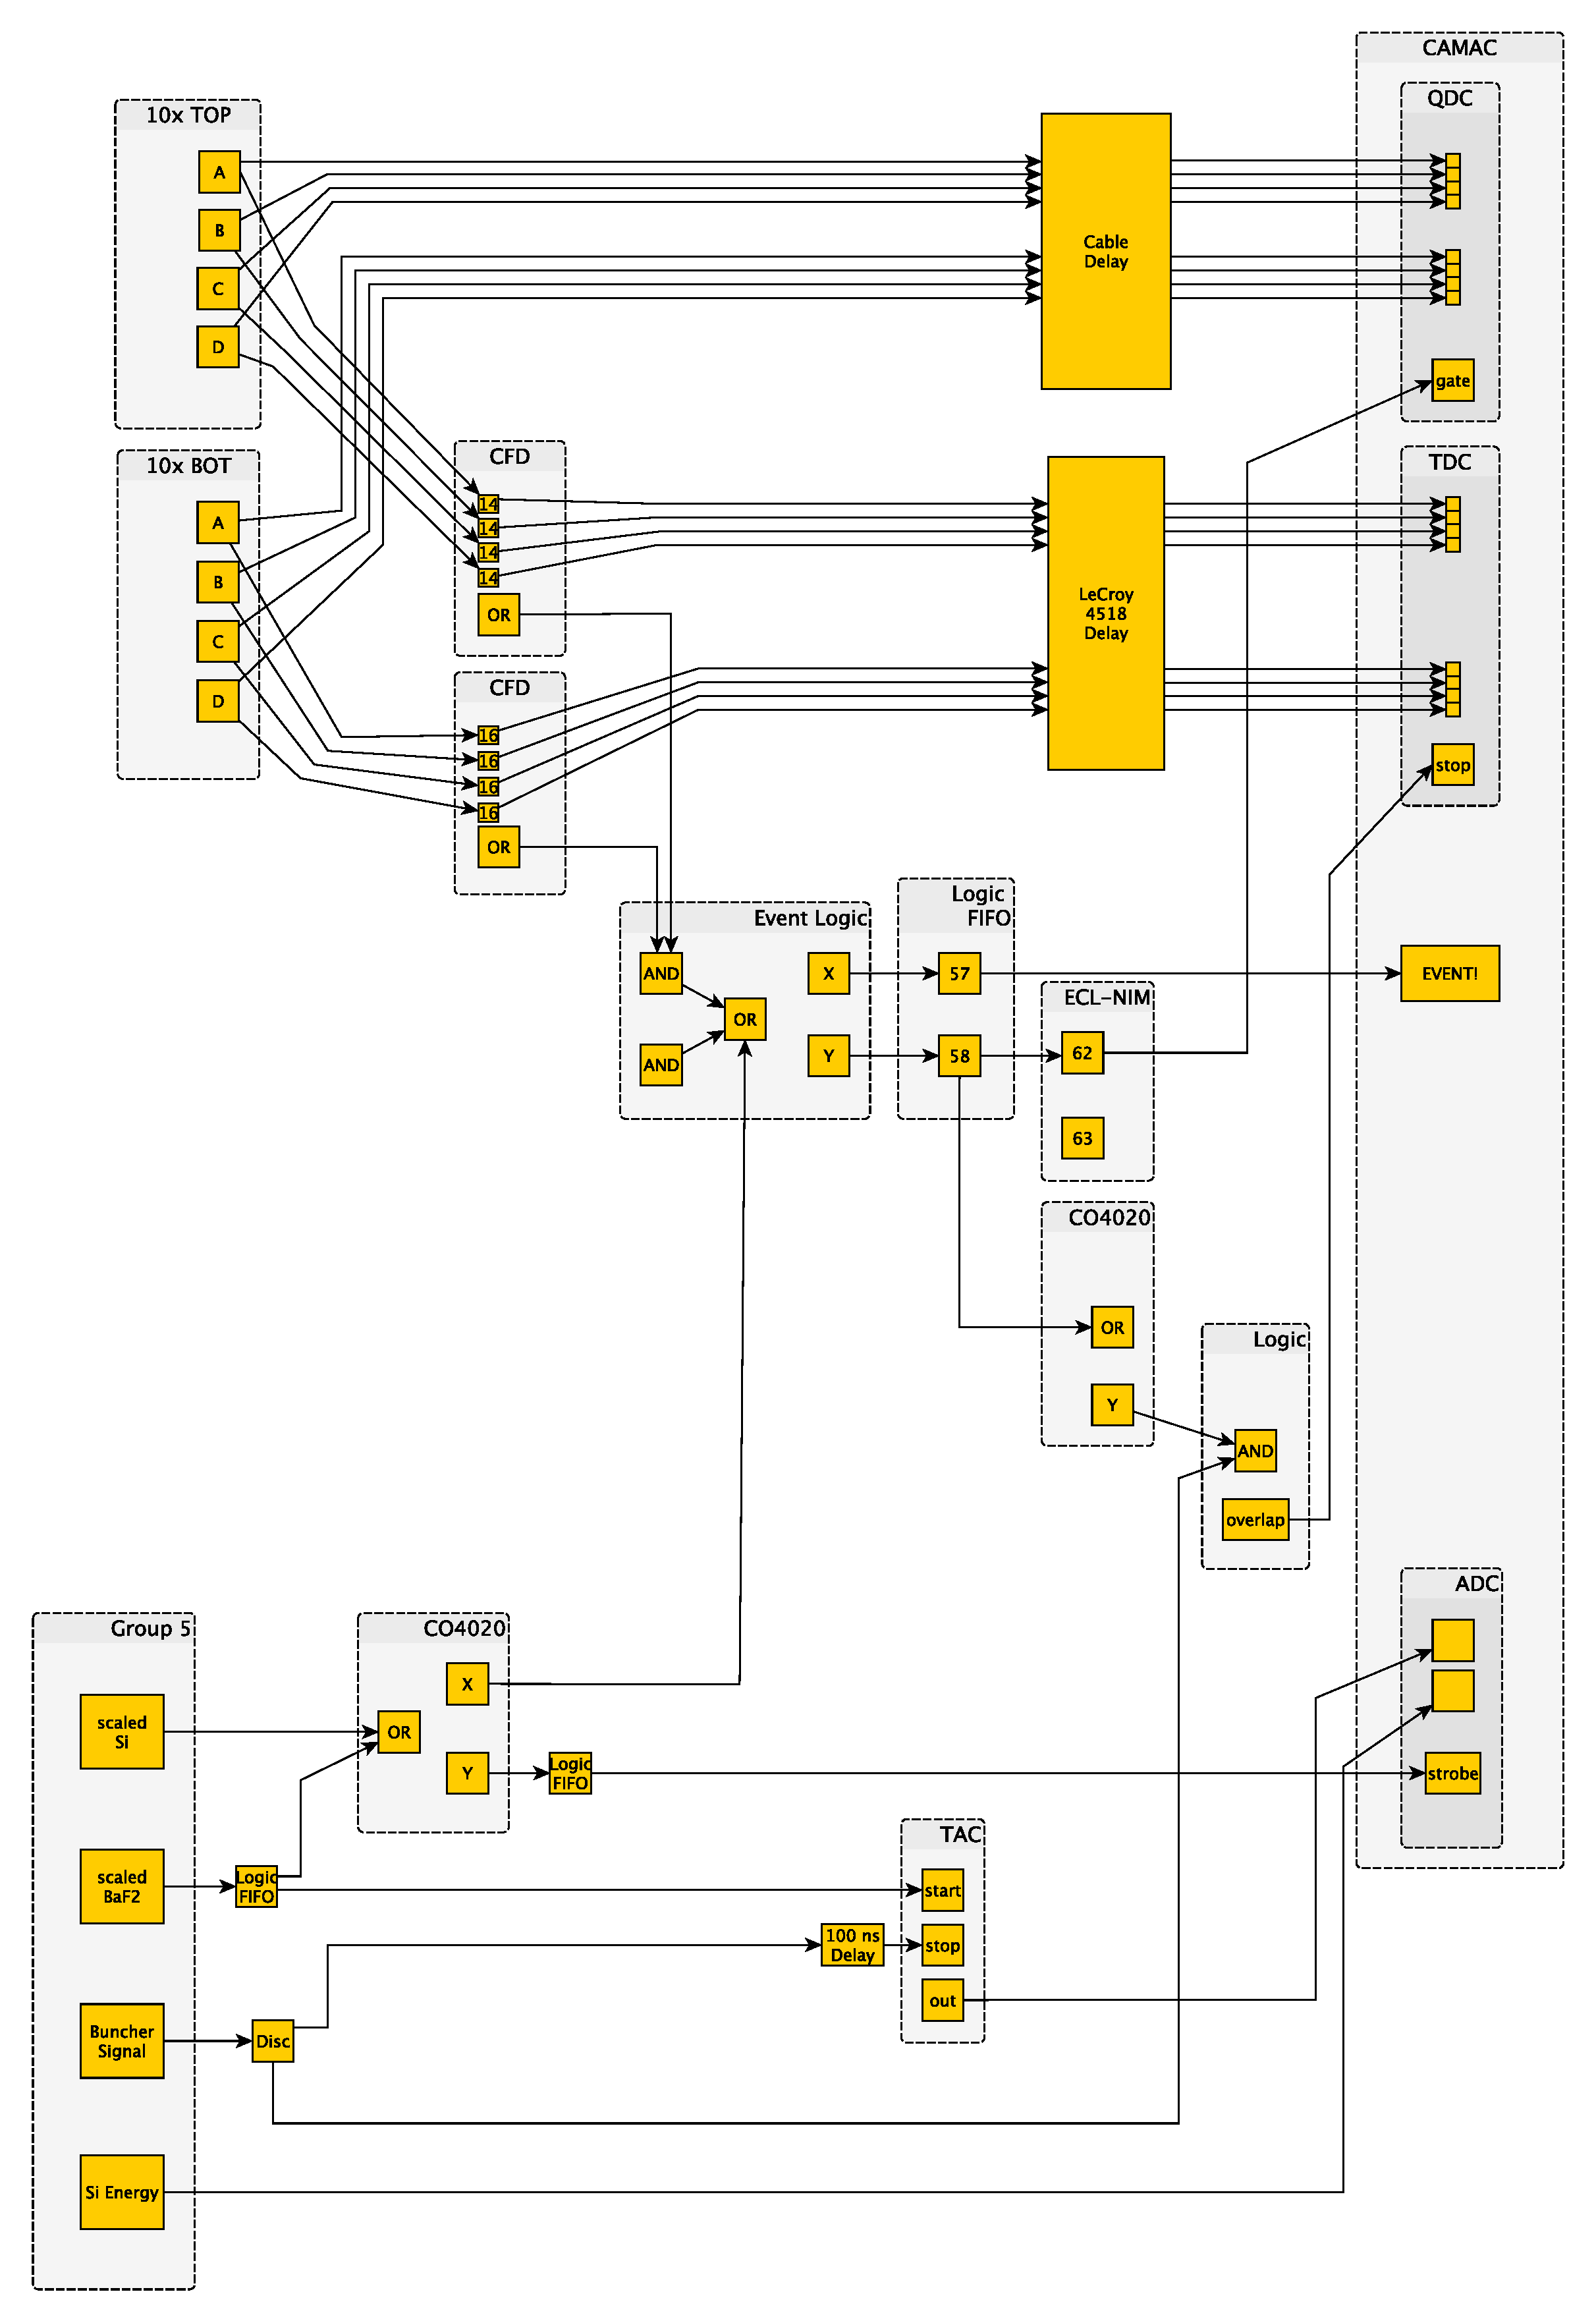
\includegraphics[height=0.8\textheight]{figures/electronics.eps}
\caption[Full diagram of the detector electronics.]{A diagram of the neutron detector electronics.  The modules on the right are read by the DAQ.}
\label{fig:fullElectronics}
\end{figure}

The DAQ must also record some quantities that are independent of the event trigger, such as the charge on the Faraday cup, which is needed to normalize the number of particles incident on the target between runs.  The DAQ records these as scalers.  {\fig}~\ref{fig:scalerElectronics} shows all the scalers that are recorded; many of these, such as the detector rates, are used only for monitoring during the run.  However, the live time and the charge are both used in the analysis.  The live scalers are important to record because the DAQ cannot collect new events while it is processing an event, and it is the live integrated beam current that is appropriate for cross-section calculations.  Measuring the live version of any scaler is possible using the busy signal the DAQ itself provides.  The busy signal is a NIM logic pulse that is low when the DAQ is busy.  Vetoing any scaler signal with this busy signal gives the live scaler, which is recorded in addition to the un-vetoed scaler.  The schematic is shown in {\fig}~\ref{fig:scalerElectronics}.  To turn the charge collected on the Faraday cup into a NIM signal that is compatible with the DAQ scaler, the Faraday cup is connected to a module that outputs a NIM logic pulse at a frequency that is proportional to the input charge.  This signal, like all the others, is recorded in both its raw and vetoed form.
% figure: Si, Q.live, NaI accumulation
% figure: full electronics
\begin{figure}[htp]
\centering
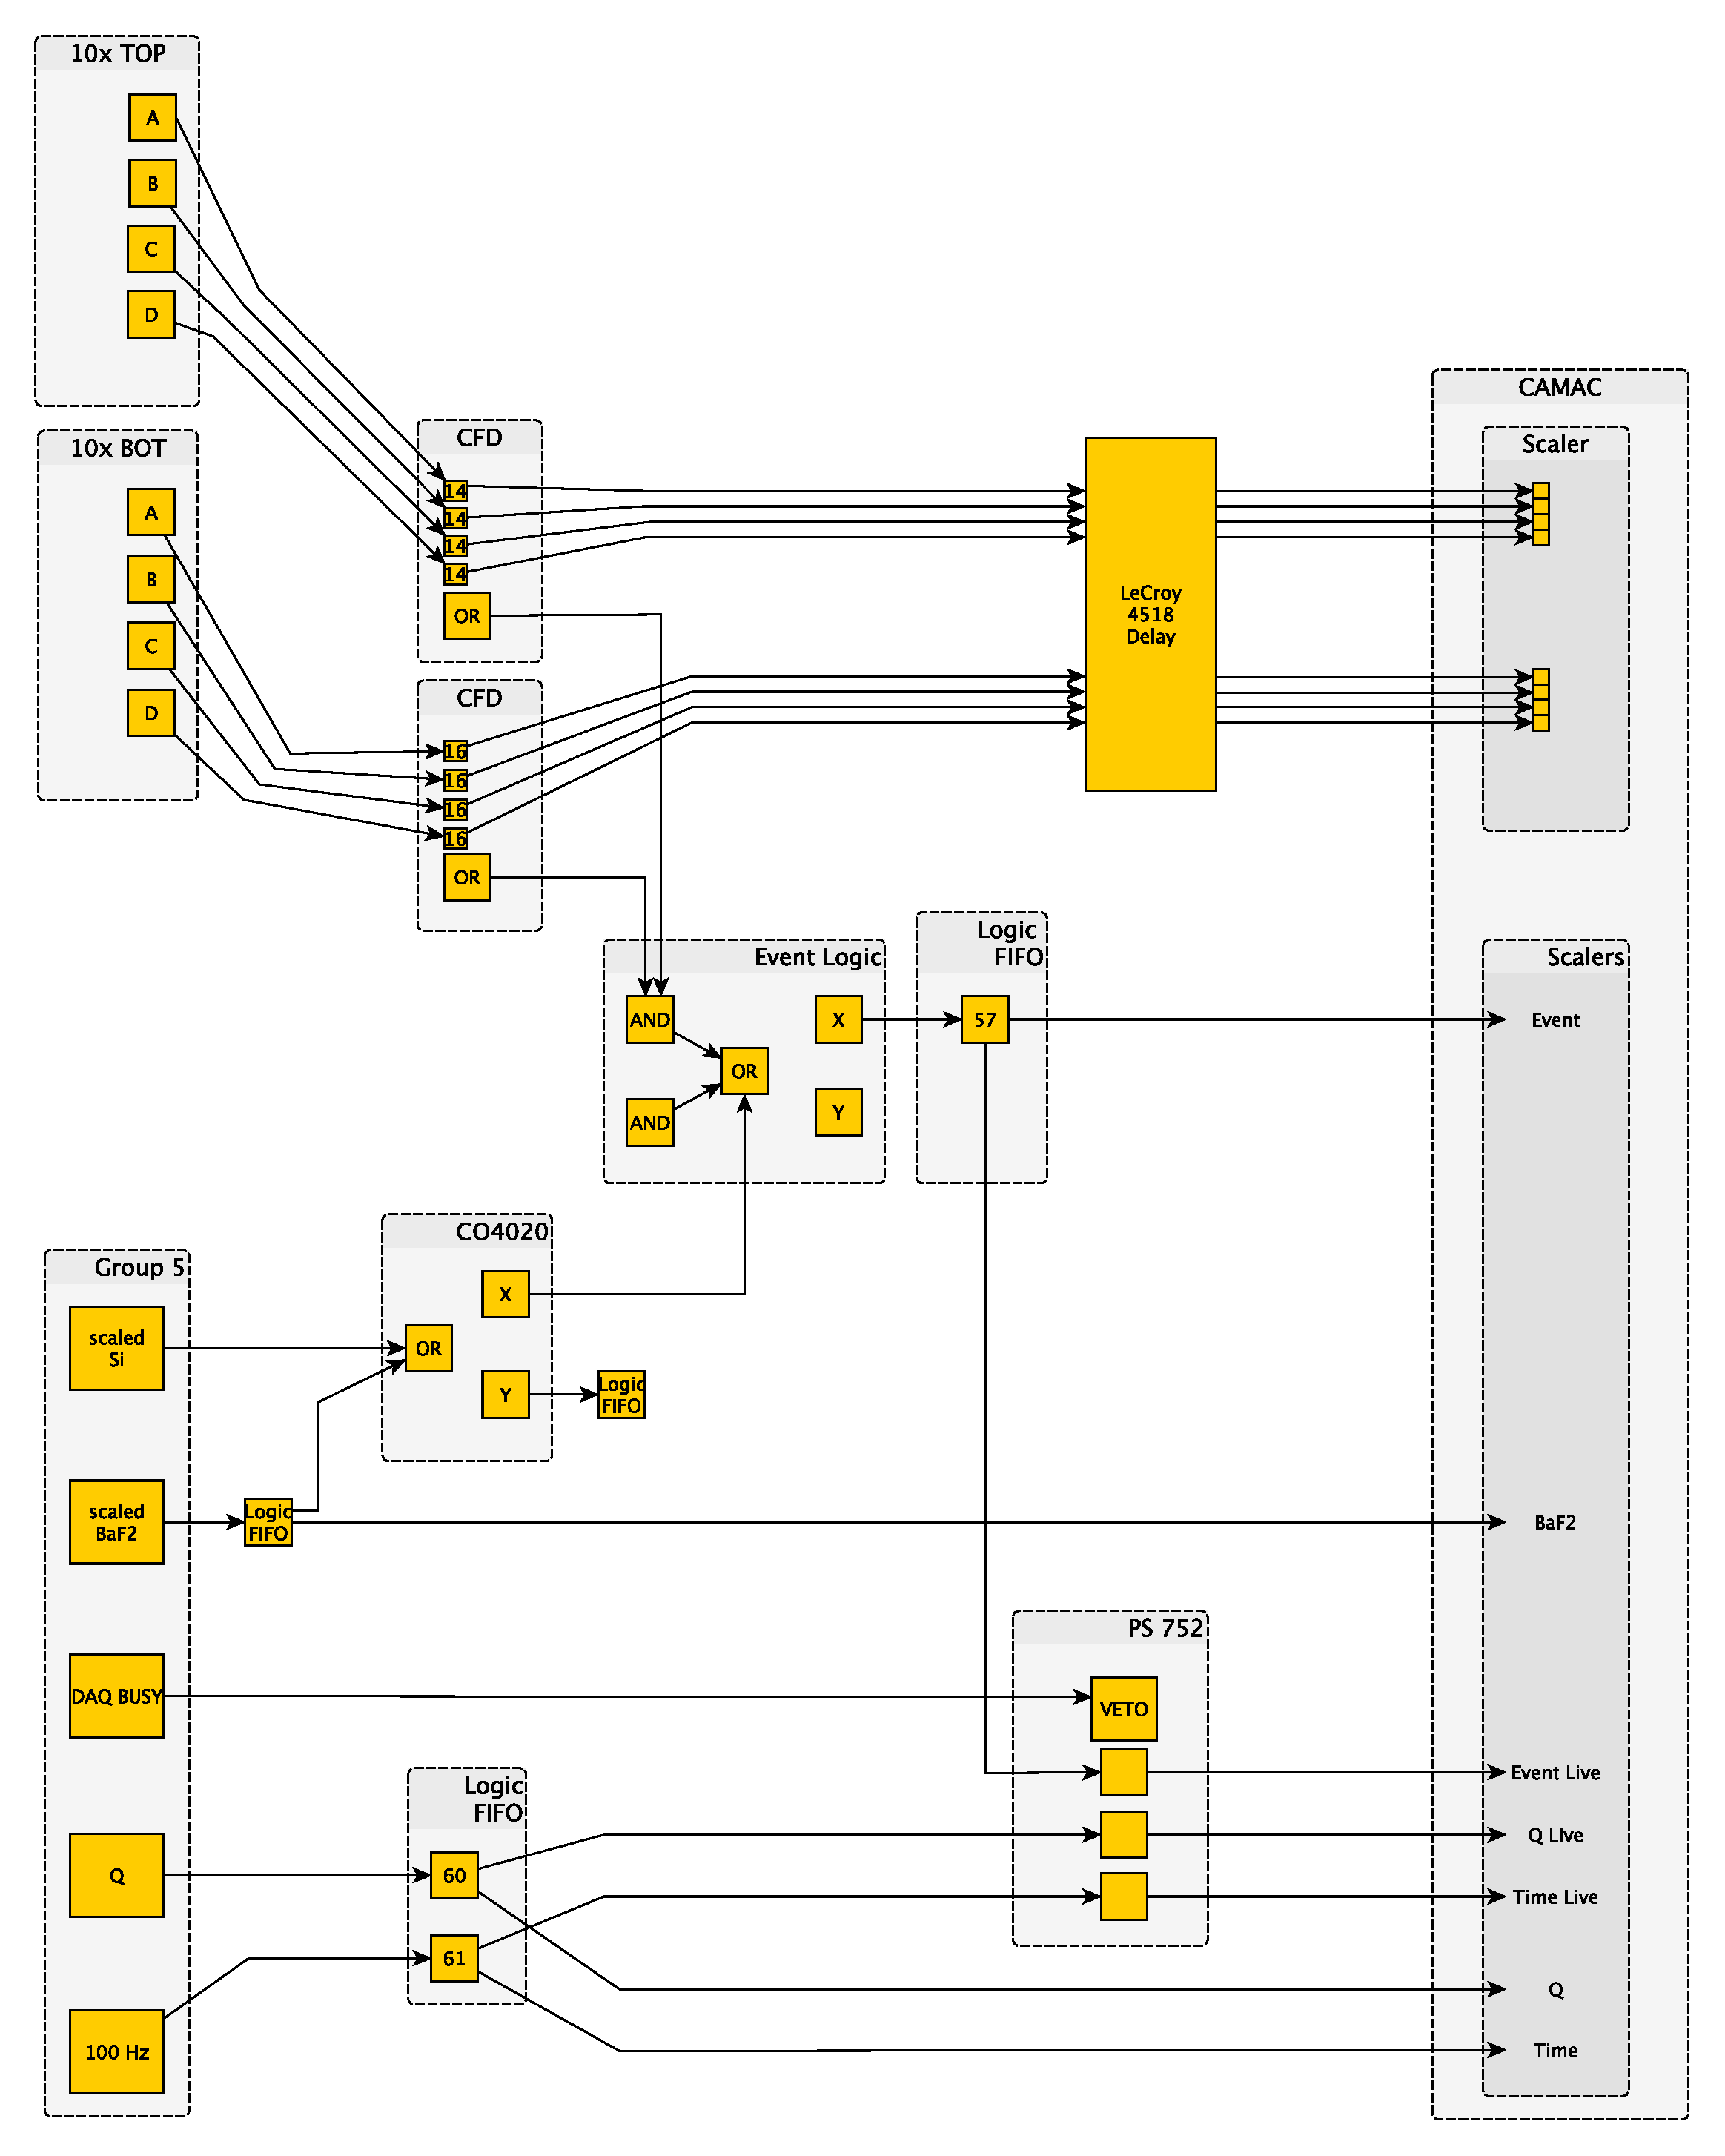
\includegraphics[height=0.8\textheight]{figures/electronics_scalers.eps}
\caption[Detector scalers.]{A diagram of the neutron detector scalers.  The modules on the right are read by the DAQ independent of the event signal.}
\label{fig:scalerElectronics}
\end{figure}
A test of this electronics setup using a \Mg{26} target verified the expected DAQ operation.  This test is discussed in the next chapter. 

% % uncomment the following lines,
% if using chapter-wise bibliography
%
% \bibliographystyle{ndnatbib}
% \bibliography{example}




%
% Chapter 4
%

%
% Modified by Sameer Vijay
% Last Change: Wed Jul 27 2005 13:00 CEST
%
%%%%%%%%%%%%%%%%%%%%%%%%%%%%%%%%%%%%%%%%%%%%%%%%%%%%%%%%%%%%%%%%%%%%%%%%
%
% Sample Notre Dame Thesis/Dissertation
% Using Donald Peterson's ndthesis classfile
%
% Written by Jeff Squyres and Don Peterson
%
% Provided by the Information Technology Committee of
%   the Graduate Student Union
%   http://www.gsu.nd.edu/
%
% Nothing in this document is serious except the format.  :-)
%
% If you have any suggestions, comments, questions, please send e-mail
% to: ndthesis@gsu.nd.edu
%
%%%%%%%%%%%%%%%%%%%%%%%%%%%%%%%%%%%%%%%%%%%%%%%%%%%%%%%%%%%%%%%%%%%%%%%%

%
% Chapter 4
%

\chapter{MUON VETO DEVELOPMENT}
\label{chap:muVeto}
\begin{comment}
Explain some cosmic ray basics - only the stuff relevant to our detector (1 muon per square foot per second and MIP -> landau energy distribution).
Discuss materials available for veto and basic design decision of WLS
\end{comment}

\subsection{Testing with 26Mg}
\begin{comment}
Show results from first run and look at timing - hey it's all right!
Look at background - will need to improve
\end{comment}

\GeTargets cross-sections are predicted to be 300 mb, much lower than previous cross-sections measured with the neutron wall.  \Mg{26} has a cross-section of ?? mb and its differential cross-section (right word?) has been well measured by \cite{Bohne_Mg}.  Since its level structure is similar to \GeTargets in that is has a low-lying 0+ first excited state, \Mg{26}(\He{3},n) serves as an excellent system to test the neutron wall.

% figure: 26Mg level scheme (along with Ge level scheme?)

The TOF spectrum at the forwardmost angle is shown in Figure ??.  The neutron peak has a width of 1.2 ns and is clearly visible against the background.  Figure ?? shows the agreement of the extracted cross-section to previously measured data.

% figure: Bar A TOF spectrum

% figure: 26Mg cross-section compared to old data

The concerning thing about this data is that the neutron peaks at angles with low cross-sections do not stand significantly above the random background.  This has serious implications for the \GeTargets experiment, where the cross-section is suspected to be even lower.  Current data on two-proton transfer typically has errors no worse than 20\%; to achieve such errors it is necessary to either reduce the background or increase the beam current.  Increasing the beam current substantially was not feasable because of ion source limitations.  The background comes primarily from low-energy $\gamma$ radiation from the cement in the room and from muons produced by cosmic rays.  The next chapter discusses the construction of a cosmic-ray veto.

% introduction to cosmic rays
Sea-level radiation due to cosmic rays consists primarily of muons created in the upper atmosphere.  The energy distribution of muons incident on the neutron detector peaks at 100 GeV/C \cite{PDG}, so that most of the muons traveling through the detector are Minimum Ionizing Particles (MIP's).  This means that their energy loss is proportional to their path length in that material.  Muons at these energies deposit 1 MeV/cm2/g \cite{PDG}.  The detector consists of plastic with a density of ??, so the muons can deposit less than 0.5 MeV to 80 MeV depending on their path through the plastic.  It is possible to discard events that are more energetic than the highest-energy neutron, but most events deposit less energy and, if they arrive in the time window of interest, are indistinguishable from a neutron event.  The rate of such muons is low; one muon per square foot per second.  Of these, only a fraction arrives in the time window of interest, 20/400.  With a high flux of event neutrons, this background would pose little problem.  But the 76Ge(3He,n) cross section is predicted to be on order of ?? mb/sr.  Without vetoing the cosmic rays, the signal will be outnumbered ?? to 1, greatly increasing the uncertainty in the absolute cross-section. 

Impractical solutions to muon background abound.  One may wish to go deep underground, giving the muons more time to decay and thus reducing their flux.  This is not feasible because the ion source and accelerator infrastructure necessary to do this experiment do not currently exist in any underground laboratory.  Another solution would be to remake the neutron detector, using a material that can distinguish between neutron and muon interactions.  Such scintillators exist [CITE!], but are typically toxic, flammable, liquids.  A large-angle detector made of such scintillator would be doubly helpful because these scintillators can distinguish between neutron and $\gamma$ radiation, as well, which would reduce another significant source of background signal.  Working with such difficult material, however, was beyond the scope of this project; the goal was to make a manageable change to the existing detector to reduce muon background. 

A practical solution to the muon background is to make a veto shield that registers the likely presence of a muon.  The events identified as muon events can then be discarded.  Distinguishing between muons and non-charged particle interactions using additional scintillator material is possible because of the difference in likelihood of interaction.  
\begin{figure}[hp]
\centering
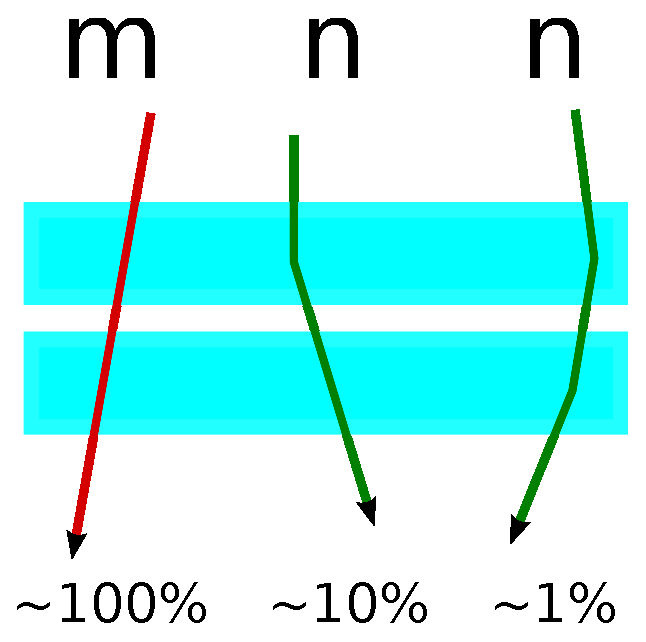
\includegraphics[width=0.4\textwidth]{figures/simpleVeto.eps}
\caption{The charged muon has a nearly 100\% chance of leaving a detectable signal in both scintillators, while the neutron, lacking charge, is much less likely to interact in even one of the scintillators.  The likelihood of detecting a neutron interaction depends on both the thickness of the scintillator and the threshold of the detector; for a 5 cm thick scintillator with a threshold at approximately the Th edge, the likelihood of detecting a 20 MeV neutron is about 10\%.}
\label{fig:simpleVeto}
\end{figure}
While the charged muon will almost certainly leave a detectable signal in both scintillators, the neutron is highly unlikely to do the same.  The bars of the neutron detector are 5 cm thick; the chance of detecting a 20 MeV neutron when the detection threshold is at approximately the Th edge is 10\%, making the chance of a neutron interacting in two bars only 1\%.  If the muon veto is made of a thinner bar of scintillator, the probability of a detectable neutron interaction in both drops further.  By placing a thin ($\sim$1 cm) scintillator over the neutron detector bar, it is possible to identify muons to an accuracy of at least 99\%.  Note that such a veto does not identify $\gamma$ radiation because it has an efficiency similar to neutrons in BC408.

\section{Light Collection with WLS}
\begin{comment}
Describe light collection with WLS
Explain why we loop the WLS and collect light from both ends
Discuss the light limitations of light guides (Liouville) and ways to increase light collection with WLS (more!)
Describe fragility of WLS, how some efforts make custom plastic clamps to make it robust, how this doesn't work for you so you made a break and attached a cable.  Discuss signal loss.
\end{comment}
The scintillator bars of the neutron detector are outfitted with two PMT's, each coupled to its end via a non-scintillating light guide.  Having two PMT's is essential both for good timing information and also to lessen the position sensitivity of the signal.  Instrumenting the veto scintillators in this way was not feasible.  Fitting a top and bottom PMT to each veto bar would require 32 PMT's and lightguides, along with independent power supplies for each.  Instead, wavelength-shifting fiber (WLS) was chosen to collect the light.

WLS collects light by absorbing broad-spectrum radiation and re-emitting that light in the green.  It is possible to coat the fiber with material with an index of refraction that guarantees total internal reflection for green light, and so the light bounces in the fiber until it reaches a detector.  WLS largely eliminates position sensitivity because it can be arranged on the detector so that no part is distant from the collecting fiber [cite??].  Because the fiber is fairly flexible, its pattern on the detector can be designed so that the fiber exits the plastic in a single bundle, allowing instrumentation with only one PMT.

Possible disadvantages to WLS are signal intensity [cite??] and fragility of the fiber.  Sufficient light intensity to boost the signal above the noise is a serious concern, and can be overcome by using many WLS strands to collect light [cite NASA thing, show picture?].  The fragility of the WLS is more difficult to remedy.  To maximize light collection, the fiber on the detector should bee taken directly to the PMT, which should be as close to the plastic as possible to minimize signal attenuation.  In some designs [CITE!], this is acheived by enclosing the fiber run to the PMT in a stiff cast.  The design for the neutron wall needed flexibility in PMT placement, making a fixed support between the detector and PMT impractical.  Several attempts were made to run the WLS collection fiber directly from the scintillator to the PMT, but even with careful handling, the fiber quickly degraded and eventually snapped.  Such degredation would have left no way to access the veto's signals and was unacceptable.  The decision was made to sever the WLS at the end of the plastic and make a robust cable to attach to the WLS and carry the signal to the PMT.  While severing the WLS causes significant light loss, it ensures durability.  The details of this design are discussed in the next section.  

\section{Paddle Design}
\begin{comment}
Schematics
Tolerances
Making sure the transmit cable lines up with the paddle WLS fibers!  Dowels.  Tolerance doesn't actually need to be that good
connecting cable with PMT
cable design - hosing for protection
\end{comment}

The main components of a veto paddle are the scintillator and WLS, which does the actual detection, the endpiece that glues onto the scintillator, which fixes the position of the WLS coming off the scintillator, and the cable, which connects to the WLS and carries the signal to the PMT.  Each piece is discussed in this section.

The scintillator material itself is $\sim3/8$'', thinner than the bars of the neutron detector.  This is desirable because we don't want the neutrons to interact with material other than the neutron detector, but the thin material can still be efficient at detecting muons.  The fiber is glued to the paddle in a ``U'' shape as in {\fig}~\ref{fig:paddle}.  This is done to maximize light collection.  Light absorbed by the fiber propagates in both directions along the fiber axis; if one end of the fiber terminates, the light must reflect off the surface and travel back to the PMT, and light loss occurs both at the reflection and there's attenuation along the path.  Light loss at the terminating surface can be lessened somewhat with the application of reflective paint [CITE] and more so by silvering the surface [CITE], but a simpler method of recovering the light is to loop the fiber on the scintillator so that both ends can terminate at the PMT, allowing collection of light regardless of its travel direction.  With such a design, care must be taken to avoid extreme bending of the WLS, as it is easily damaged.  The bend radius chosen was ?? cm, which seemed to have no adverse effect on the WLS.

In general, the design goal was to maximize light collection while ensuring durability.  We could see that occasionally there was a default in the WLS cladding and were concerned that some fiber would suffer from more light loss than others.  The solution, using multiple strands of fiber to collect light, was intended to buffer the detector from chance defects in the WLS.  Using multiple strands of fiber also increases light collection, as found in [CITE!].  In general, light collection increases as more WLS is added to the surface, and there is not noticable position sensitivity if no part of the scintillator material is more than $\sim$5~cm from WLS fiber.  While more fiber could have been added to the surface of the scintillator, it already covered the surface and provided sufficient signal, shown in {\fig}~\ref{fig:vetoSignal}.  Furthermore, the WLS was glued into a channel machined into the scintillator to keep it from being damaged.  While more WLS fiber could increase the light collection, increasing the fiber on the surface would have meant machining away more scintillating material.  We did not want to reduce the possible energy deposition of the muons, as this was already quite low due to the thinness of the scintillator.

An endcap fitted to the scintillator helps protect the WLS and also ensures the WLS location, allowing good alignment to the fibers in the cable.  The endcap minimizes possible WLS flexing by connecting to machined indents in the scintillator with a press fit.  Because the endcap extends into the scintillator, bending the fiber perpendicular to its axis is essentially eliminated.  Scintillator is also machined away from the fiber's entrance to the endcap to avoid point pressure.  Once the endcap is slid onto the scintillator, it is glued in place, not to secure it to the scintillator, but to fix the WLS in their holes completely so that the surface of the endcap can be polished without damaging the WLS.

The cable that transmits the light from the WLS to the PMT has three seperate parts.  A connector mates with the endcap attached to the scintillator and connects to the tubing, which is 2~m long and connects to a connector that attaches to the PMT.  At each interface between tubing and connector, the primary concern is that the stresses on the transmission fiber be small enough to not damage the fiber.  A hose barb attached to each connector allows the transmission fiber through and also allows the tubing to firmly connect without putting strin on the fiber.  Slightly stiff tubing (durometer rating = ??) was chosen to help limit the bend radius of the cable, further protecting the transmission fiber.  

The primary concern for the portion of the cable that attaches to the endcap is that each transmission fiber completely overlap its WLS fiber.  The diameter of the transmission fiber is ??~mm, larger than the ??~mm-diameter WLS fiber, which allows misalignment of ??~mm without greatly impacting light collection.  Tight-fitting dowels help align the region of the cables containing the fiber cluster.  This is particularly important because the connectors are machined from plastic and are not perfectly square - some connectors bow as much as 20 mils from normal.  The only regions that must be carefully aligned, however, are the fiber clusters, and the dowels constrain these regions to less than ?? mils, ensuring an alignment of ?? mm.

\begin{figure}[htp]
\centering
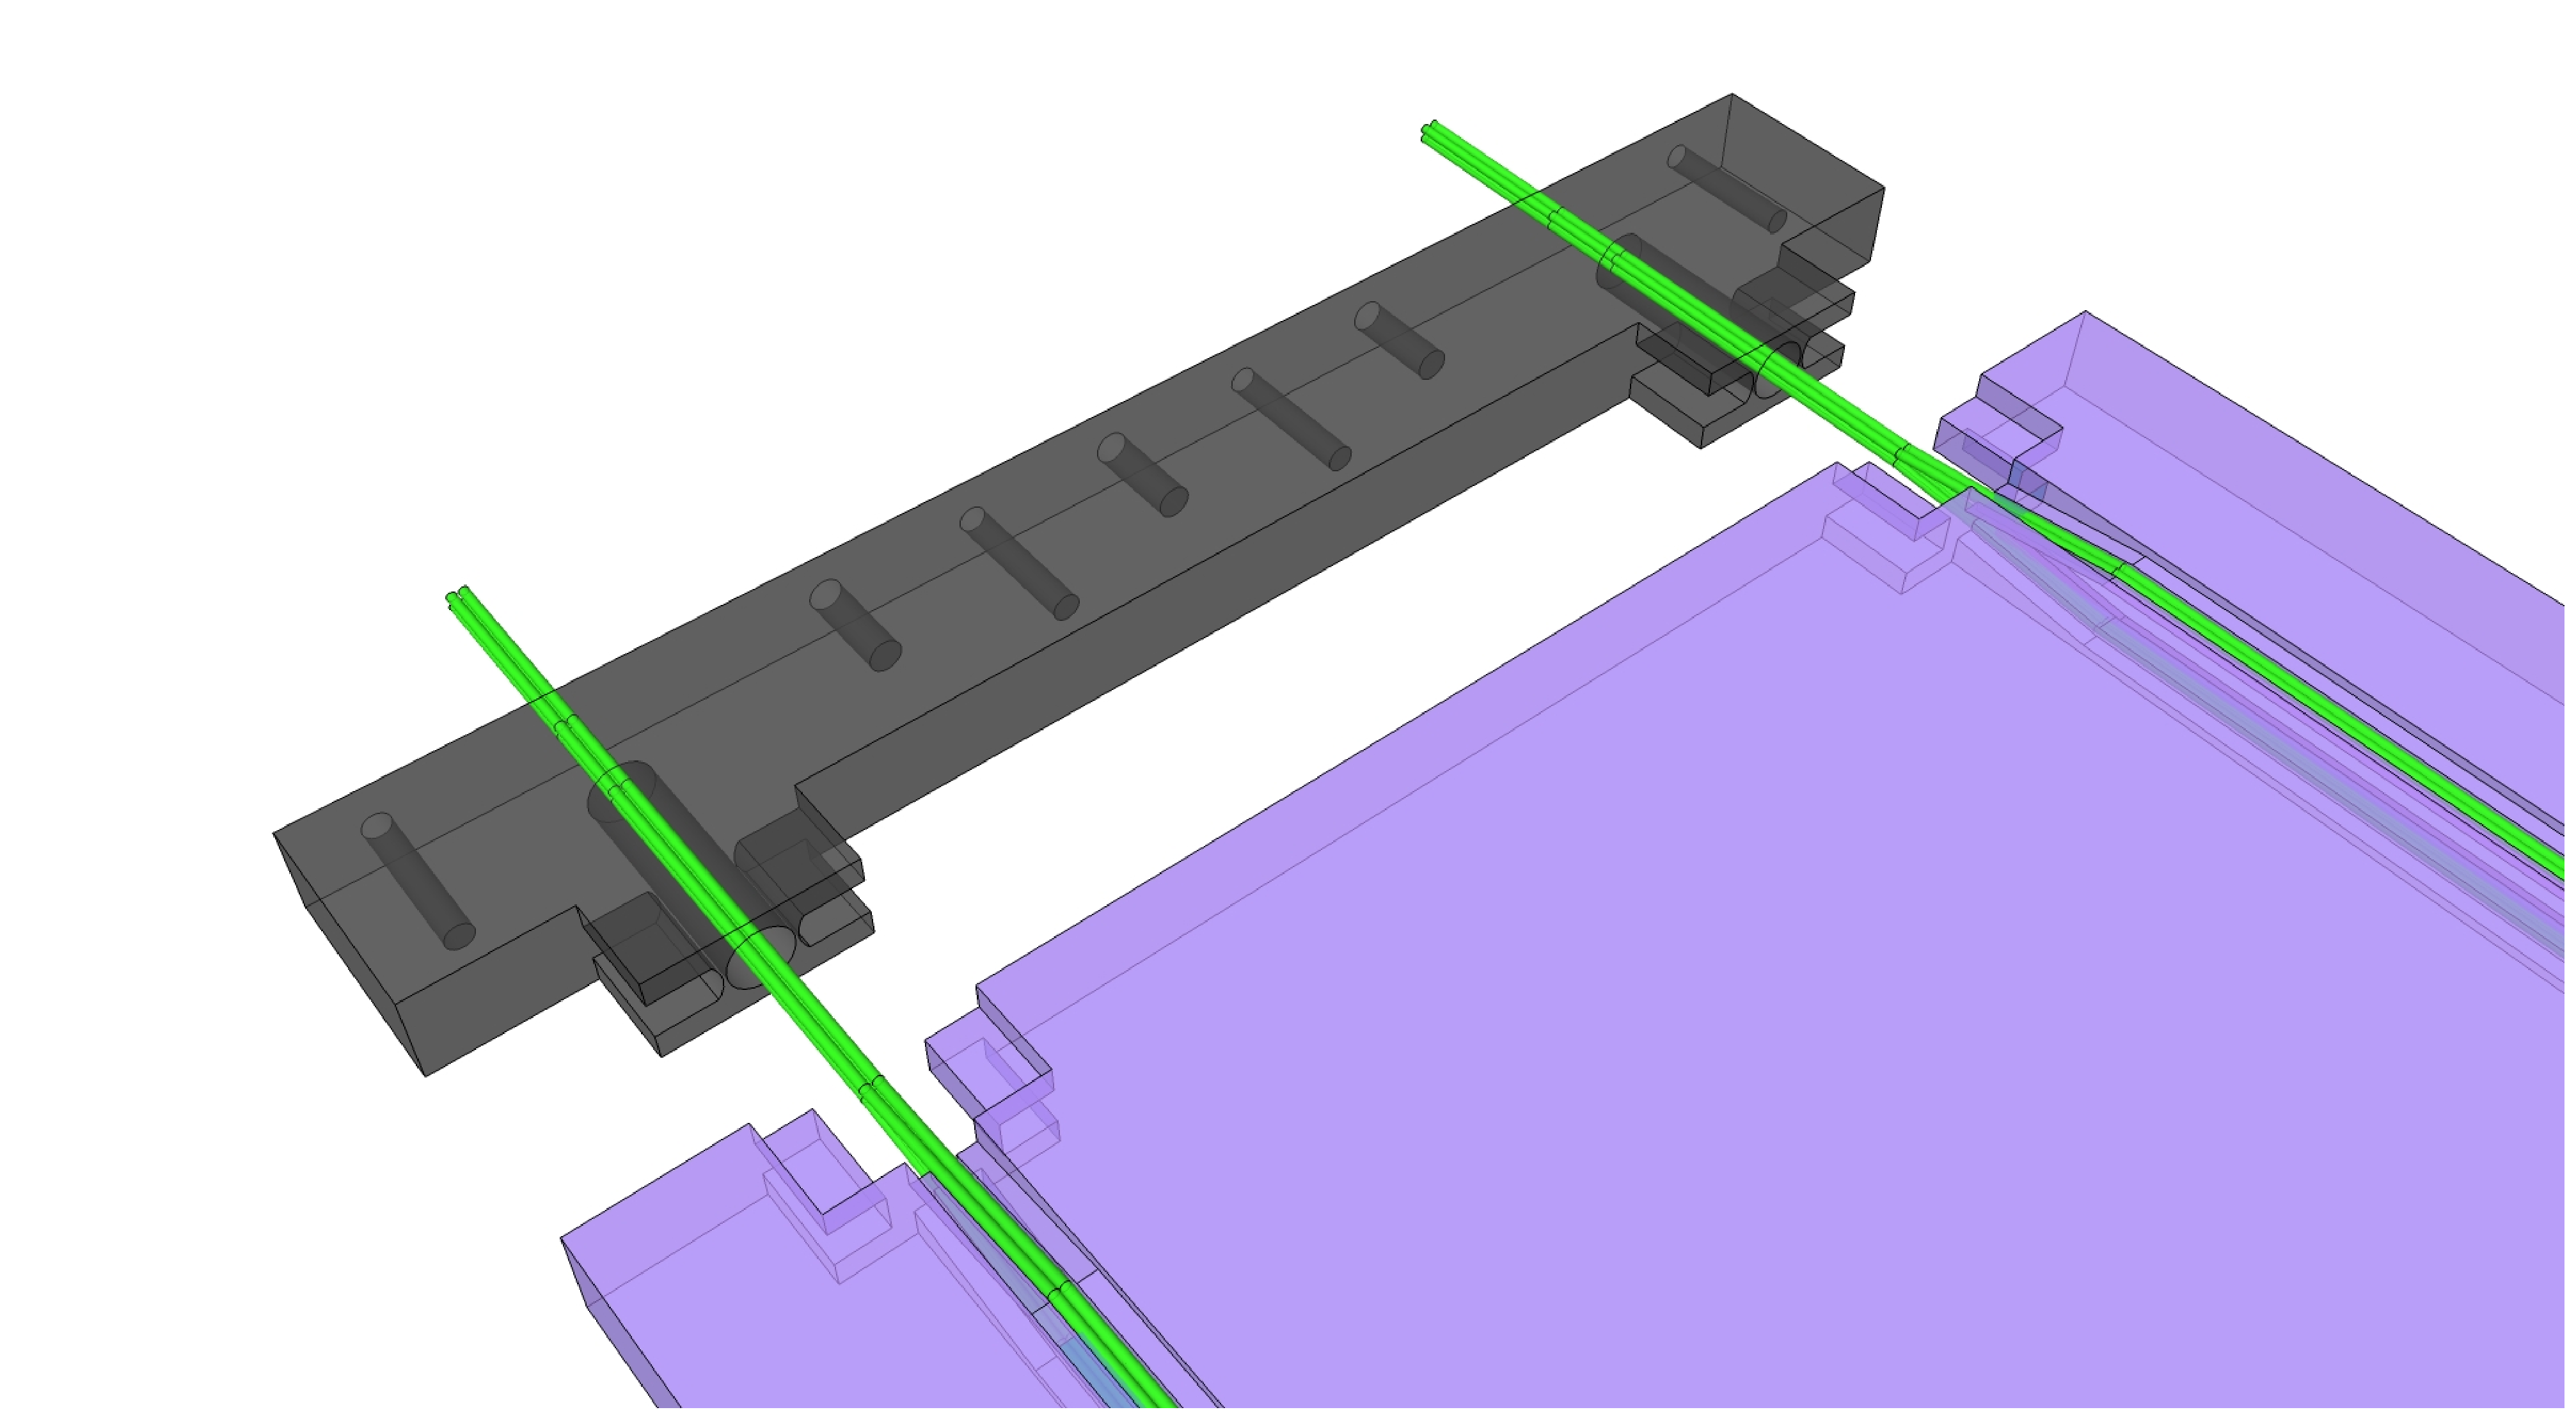
\includegraphics[width=1.0\textwidth]{figures/veto_assembly.eps}
\caption{The endcap will be glued to the scintillator after it is slid into place.}
\label{fig:paddleAssembly}
\end{figure}


\section{Paddle Performance}
\label{sec:singleVeto}

\subsection{tests on intrinsic efficiency}
\begin{comment}
Show signal from detector
Talk about first tests?  Can talk about sensitivity to geometric alignment of trigger paddles ...
Maybe mention this and then be like, ``this is why we decided to look at the efficiency this other way that was less sensitive''
except you weren't able to do further tests so you'll just have to say the limits you got
\end{comment}
The intrinsic efficiency of the paddles can be tested by requiring a coincidence with several paddles.  The several-detector coincidence identifies signals as muons.  If the coincidence paddles are arranged so that the path of any muon intersecting all the veto paddles must also intersect the volume of the veto paddle, the efficiency measured is the veto's intrinsic efficiency, separated from its geometric coverage of whatever detector it is vetoing.

In practice, arranging the available scintillator to force muons through the test volume was difficult because the available scintillator was instrumented with bulky lightguides and could not be laid directly on the test volume.  A simple cosmic ray simulation program helped determine an arrangement that maximized geometrical efficiency.  This arrangement, however, was extremely sensitive to placement; measured efficiency of the same bar could change from 98\% to 75\% with a displacement of a few centimeters.
\begin{figure}[htp]
\centering
\includegraphics[width=1.0\textwidth]{figures/efficiency_test.eps}
\caption{This arrangement of coincidence material ensures that muons triggering all coincidence detectors must also travel through the veto paddle.}
\label{fig:efficiencyTest}
\end{figure}

The efficiency was measured by counting how often the veto paddle had a detectable signal when all the coincidence material registered a coincidence.  Assuming the muon was constrained to travel through the veto paddle volume, the ratio gives the efficiency.  The DAQ Event signal was a logic pulse resulting from the coincidence of the coincidence paddles.  This logic pulse also acted as a Start for a TAC.  The TAC stop signal was a delayed, discriminated veto paddle signal.  The outgoing TAC signal was sent to an analog to digital converter (ADC) for integration.  Signals from the veto paddle coincident with the other scintillators show up in the timing spectrum as a peak at the time of the delay.  The integral of this timing peak divided by the number of event triggers gives the efficiency.
% figure: the considerably complicated spectrum
\begin{figure}[htp]
\centering
\subfloat[][]{
   \includegraphics[width=0.45\textwidth]{figures/vetoTest_electronics.eps}	
}
\subfloat[][]{
	\includegraphics[width=0.45\textwidth]{figures/vetoTest_timing.eps}
}
\caption{The location of the timing peak is set by the delay introduced to the discriminated veto paddle signal.  Integrating the timing peak gives the number of muons that generated an observable signal in the veto paddle.}
\label{fig:vetoTestElectronics}
\end{figure}

Testing the efficiency of the veto paddle with this setup was not ideal because the geometrical efficiency was very sensitive to the placement of the coincidence detectors; measured efficiency of the same bar could change from 98\% to 75\% when one of the coincidence detectors was shifted by as little as a few centimeters.  However, this setup was useful in testing the effect of the cable polishing, cable out-of-true-ness, and the condition of the plastic scintillator.  In general, all efficiency measurements fell between 94\% and 98\%: even the veto paddles made of the most badly damaged plastic were as efficient as the veto paddles made from the plastic in excellent condition.  No statistically significant differences were seen between cables with the most and the least amount of bowing.  Polishing the cables with the bull-nose single-crystal diamond increases detection efficiency by $\sim2$\%, although it should be noted that the change may have been due to correlated noise in the system rather than to improved light transmission.  The discriminator threshold, set to its lowest value, gave an efficiency of 98\% compared to 94\% when set to its highest value.

Testing the position dependence of the efficiency using the setup described above was not practical due to its sensitivity on positioning.  Instead, the response of the veto paddles to a loosely collimated $\gamma$ source was tested.  Counting detected $\gamma$ radiation showed a deviation of less than 8.5\% over the veto paddle.  While this is not a measurement of the position dependence of the muon efficiency, it does limit the efficiency change over the paddle since muons typically deposit at least double the energy of the $\gamma$ radiation from the $^{60}$Co source.  See {\fig}~\ref{fig:positionDependence} for the variation of the efficiencies.
\begin{figure}[htp]
\centering
\includegraphics[width=1.0\textwidth]{figures/vetoTest_positionDependence.eps}
\caption{The dependence of the number of detected events on the position of a loosely-collimated $^{60}$Co source.  The spread is approximately 8.5\%.}
\label{fig:positionDependence}
\end{figure}


\subsection{On-Detector Efficiency}
\begin{comment}
Initial efficiency - would be nice to show this data
Describe different cosmics that hit the neutron bar but miss the veto - argh!
Discuss changes made to mounting to improve coverage - show new data (cosmics)
\end{comment}
Sixteen veto paddles were initially mounted on top of the neutron detector support structure to avoid removing (and potentially damaging) the heavy neutron detectors.  Each veto paddle was $\sim$2~cm offset from a bar in the neutron detector.  Running a test with 26Mg(3He,n) showed good cosmic rejection in the two innermost bars of each four-bar unit and worse rejection in the outer two bars by about 20\%, corresponding to double the cosmic background.  The outer bars act as additional veto for the inner bars, while the outer bars enjoy no such additional vetoing.  
\begin{figure}[htp]
\centering
\includegraphics[width=1.0\textwidth]{figures/initialBackground.eps}
\caption{Room background after rejection with the initial placement of the veto paddles.  Note that the high-background bars are those on the ends of each group of four.}
\label{fig:initialBackground}
\end{figure}

A simulation of the cosmic background indicated that the geometrical efficiency was very sensitive to the distance between the veto paddle and neutron detector bar as well as the distance between the bars of the neutron detector.   The bars in the neutron detector were moved as close as the mounting screws would allow, within 1~cm.  Instead of attaching the veto paddles on top of the retaining bars on the neutron detector, they were taped to the bars and both bar and veto paddle were supported together by the same retaining bar.  The separation between the bars of the neutron detector and their veto paddle is $\sim$0.5~cm due to stiff foam placed between the two to protect the WLS channels in the veto paddles.  Material was also added to the sides of the outermost neutron detectors.  The final setup is shown in {\fig}~\ref{fig:vetoSetup}.  These changes improved both the average and uniformity of the background rejection, as can be seen in {\fig}~\ref{fig:finalBackground}.
\begin{figure}[htp]
\centering
\includegraphics[width=1.0\textwidth]{figures/vetoSetup.eps}
\caption{The final arrangement of the veto paddles on the neutron detector.  The distance between the veto paddles and the bars of the neutron detector have been minimized.  Note also the addition of veto material on the sides of the neutron detector sub-units.}
\label{fig:vetoSetup}
\end{figure}

\begin{figure}[htp]
\centering
\includegraphics[width=1.0\textwidth]{figures/finalBackground.eps}
\caption{Room background after rejection by the veto.  Note that the average and the spread are both reduced from that of the initial setup.}
\label{fig:finalBackground}
\end{figure}

\section{Electronics}
\begin{comment}
Originally wanted to use timing information but there weren't enough channels
Bit Register - give example
discuss random rate and estimate how often you'll fire during a real event and also how often one bar will fire with something real, vetoing a real event
LeCroy 4532 - MALU - majority logic unit ``The status of up to 32 inputs can be monitored and recorded by issuing a strobe.  Since the inputs are edge-triggered, the strobe may be a gate of arbitrary duration.  Then any inputs which are on during any portion of the gate are recorded and stored in a pattern register.'' (from the manual).
\end{comment}
As mentioned above in {\sect}~\ref{sec:singleVeto}, tests on single veto paddles were done using a timing spectrum.  Recording time information for the full veto was not practical, and two bit registers were used instead.  A bit register has several inputs, each corresponding to a bit in an integer, and a gate.  When the gate is high, the bit register records the bit pattern built by the voltages on its inputs; its output is the integer corresponding to this bit pattern.  This integer is a unique representation of which bars fired during the time specified by the gate.  If the gate used is the Event signal from the neutron detector, the bit register will record which veto paddles fired during an event of interest.  Two 16-channel LeCroy 4532 bit registers were able to instrument all the veto paddles.  The gate signal was a 200~ns-wide copy of the event trigger.

Recording the integer generated by the bit register instead of the time of the signal relative to the beam bunch is a loss of information.  The maximum time difference between an event in the neutron detector and an event in the veto that will still be recorded in the bit pattern is the width of the gate signal, 200 ns.  This compares unfavorably to the timing spectrum, where even with a leading edge discriminator, the timing peak has a width of less than 5 ns.  The concern is that this loss of precision in timing information will lead to unacceptable vetoing of real events.  

Several sources contribute to non-beam-related background radiation, resulting in a beam-off rate in a neutron detector bar of $\sim$1000~Hz.  While some of these events are due to muons, but they have a rate of 1~Hz/ft$^2$ and are therefore a small part of the beam-off noise rate.  The beam-off rate, then, serves as a suitable rate with which to calculate an upper bound for the rejection of beam-related events.  The probability that a noise event will occur within the window allowed by the bit register is 

\begin{equation}
\frac{Rate}{Time Window} = \frac{1000 Hz}{200 ns} = 5\times10^{-8}.
\end{equation}
With a number of triggers of approximately 10??, the expected number of rejections based on unrelated background is a scant 20?? counts.

\section{Beam Tests}
\begin{comment}
What data should I show?  Old Mg vs. New Mg?  Or New Mg with no veto vs.  New Mg with veto?
show the vetoed spectrum - put a limit on how much real signal is rejected?
\end{comment}

\subsection{Rejected Signal}
\begin{comment}
Two causes for rejected signal
1. the bars are ganged together; could get a signal in one veto bar that does not mean there was a cosmic in its adjacent neutron detector
2. randoms

can place a limit on randoms, reals, and therefore good rejected signal
\end{comment}

% % uncomment the following lines,
% if using chapter-wise bibliography
%
% \bibliographystyle{ndnatbib}
% \bibliography{example}




%
% Chapter 5
%

%
% Modified by Sameer Vijay
% Last Change: Wed Jul 27 2005 13:00 CEST
%
%%%%%%%%%%%%%%%%%%%%%%%%%%%%%%%%%%%%%%%%%%%%%%%%%%%%%%%%%%%%%%%%%%%%%%%%
%
% Sample Notre Dame Thesis/Dissertation
% Using Donald Peterson's ndthesis classfile
%
% Written by Jeff Squyres and Don Peterson
%
% Provided by the Information Technology Committee of
%   the Graduate Student Union
%   http://www.gsu.nd.edu/
%
% Nothing in this document is serious except the format.  :-)
%
% If you have any suggestions, comments, questions, please send e-mail
% to: ndthesis@gsu.nd.edu
%
%%%%%%%%%%%%%%%%%%%%%%%%%%%%%%%%%%%%%%%%%%%%%%%%%%%%%%%%%%%%%%%%%%%%%%%%

%
% Chapter 4
%

\chapter{DATA ANALYSIS}
\label{chap:dataAnalysis}
We care about two things:
1. The absolute cross-section of the ground state transition
2. Setting a limit on excited 0+ state cross-sections

error calculations: its own section?

\section{Detector Efficiency}

deuterium, Mg, cuts

\section{Experimental Parameters Related to the Cross Section}
current, tgt thickness (RBS), solid angle, dead time
go ahead and discuss errors while you discuss these quantities

The absolute cross section is the number of times a reaction occurred normalized by the total number of particles incident on the target and the number density of nuclei in the target:

\begin{equation}
\text{cross section} = \frac{\text{times reaction occurred}}{\text{particles incident on target} \times \text{number density of target nuclei}}
\text{cross section} = \frac{\text{times reaction occurred}}{\text{particle current} \times \text{time} \times \text{target thickness}}
\label{eq:cross_section}
\end{equation}

\section{Background Subtraction}

two data sets
- pulse selection
- no pulse selection

background
- gamma peaks - do not overlap with neutron peak
- other neutron peaks - ??
- randoms - background in both data sets
- continuum - more important in non-pulse-selected data

extracting counts 
- pulse selection
- no pulse selection

The data sets for this analysis were gathered in two seperate runs; the pulse selector was not working for part of the first run.  Analysis of the datasets taken with pulse selection is straigtforward and will be discussed first.  Without pulse selection, the neutron peak sits on top of background from previous neutron bunches.  The background fit is different and the total counts have a larger systematic uncertainty; extracting these will be discussed second.

\subsection{Pulse-Selected Data}
Consider the signals that build the TOF spectrum.  Random background radiation can occur at any time with respect to the beam bunch.  In fact, it should have no knowledge of the beam bunch and is equally likely to occur at every time after a beam bunch.  In other words, the TOF spectrum of background radiation should be flat.  Taking a TOF spectrum with no beam confirms this.

%figure of beam-off TOF spectrum

The neutrons coming from the ground state of \As{78} are monoenergetic and should come at a fixed time relative to the beam bunch; counts from these neutrons should form a peak that is approximately as narrow in time as the beam bunch.  Looking a a beam-on TOF spectrum, it is clear that the neutron peak and the flat background are not the only features.

% figure of beam-on TOF spectrum

The other prominant features of this spectrum are peaks from gammas produced when the beam hits the target and also neutrons from excited states as well as a broad neutron evaporation spectrum from multiple-channel interactions.

In the case of the pulse-selected data, the background that overlaps with the neutron peak of interest is well-determined.  The gamma peaks are far away from the neutron peak and have no effect.  Wonderfully, the broad, flat region ennables a very precise estimate of the random background level.  The neutron evaporation peak is the least-well understood contributor to the background of the ground state neutron peak and will be discussed later.  For now, we focus on the simplest contribution to the background, the flat distribution due to randoms.

In general, extracting the counts due to the neutrons is simple:

\begin{equation}
\text{Sum(peak region) - Background(peak region)}
\label{eq:counts}
\end{equation}

With an associated error

\begin{equation}
\sqrt{\sigma_{Sum}^2 + \sigma_{background}^2}
\label{eq:errDef}
\end{equation}

The sum of counts in a fixed region can be understood as a random variable; as such, its error is $sqrt(N_{peakregion})$.  This is quite large - is there an extraction method that will reduce this error?  The two most straightforward options available to a physicist bent on extracting counts due to a signal are sideband subtraction and fitting.  Fitting when the background is not understood can lead to systematic errors, while sideband subtraction's accuracy depends on a background that does not change rapidly near the signal region.  With these data sets, the number of signal counts is very small compared to the background.  Using sideband subtraction introduces another random variable and increases the width of the distribution of extracted counts for a given bar.  In the case of the pulse-selected data, there is no need to introduce this additional statistical error because the flat background is determined to within ??\%, so that using the fitted value is much more like introducing a constant into the equation for the extracted counts, improving the fractional error by almost a factor of $\sqrt{2}$.  See \fig \ref{fig:statDist} to see the effect of using the fitted value on the width of the extracted count distribution.

\begin{equation}
Counts = Sum(peak region) - Fitted Constant * number of Bins
\sigma^2 = Sum + fit error
\label{eq:fitErr}
\end{equation}

\begin{figure}[ht]
\centering
  \subfloat[Distribution of Background Counts][Distribution of Background Counts]{
  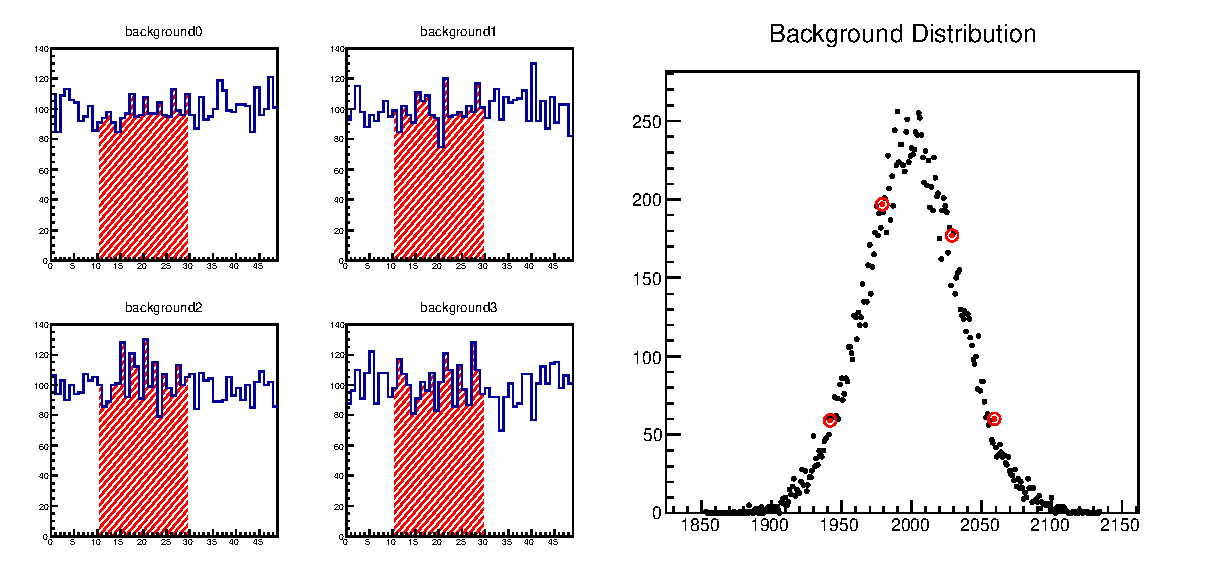
\includegraphics[width=0.3\textheight]{figures/bkgDist}
  \label{fig:bkgDist}}
  
  \subfloat[Distribution of Signal Counts][Distribution of Signal Counts]{
  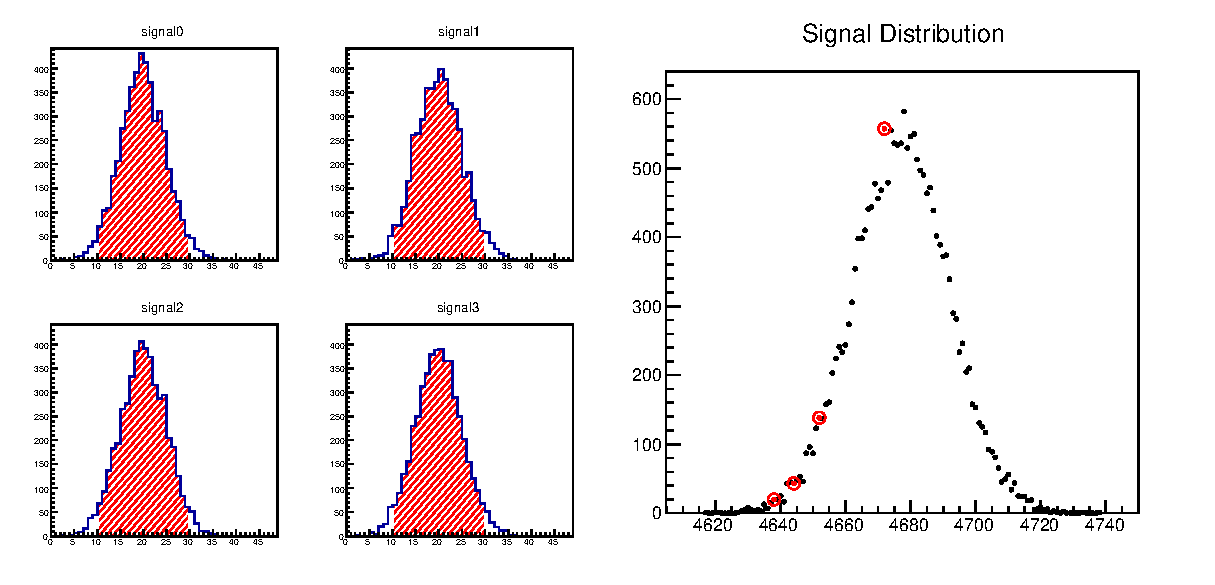
\includegraphics[width=0.3\textheight]{figures/sigDist}
  \label{fig:sigDist}}
  
  \subfloat[Distribution of Extracted Counts][Distribution of Extracted Counts]{
  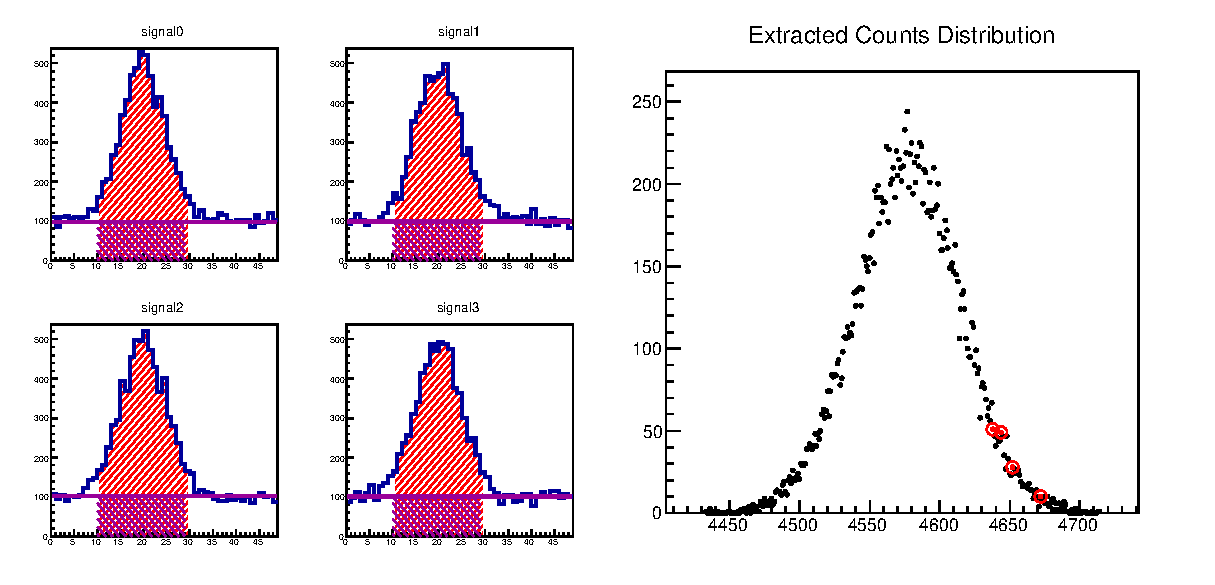
\includegraphics[width=0.3\textheight]{figures/extractDist}
  \label{fig:extractDist}}

  \caption{The number of counts in the peak region are a sum of the number of counts in the random background and counts from the neutrons.  The width of a sample at a uniform rate is simply sqrt(N), as seen in figure ??.  This is an appropriate description of the random background.  The neutron peak is roughly gaussian-shaped, and running trials where counts are drawn from a gaussian distribution shows that the width is ??.}
  \label{fig:statDist}
\end{figure}

The error introduced to the extracted counts depends on how the background is determined.  In the case of the pulse-selected data, it is clearly better to fit the background.  The constant component of the background is well-determined and contributes a tiny ??\% to the total error.  The evaporation spectrum is not as well constrained and introduces ??\% to the total error.  Even with the uncertainty in the evaporation spectrum fit, the improvement in the error compared to sideband subtraction is a factor of ??.

\subsection{Pulse-Selected Data}
With pulse selection, the region behind the neutron peak has only random signal and can be fit with a constant to within ??\%.  Assuming that the neutron peak itself does not overlap with other background, the total number of counts is estimated as the direct sum of the bin contents minus the average bin content of the background region.  In this case, the error should be the statistical error associated with the random background in the peak region and the statistical error associated with the counts in the neutron peak, added in quadrature.  Such an error neglets the error associated with the constant that is fit, appropriate in this case because it influences the error by at most 0.1\%.

When considering the error, it should be considered that the neutron peak itself may be sitting on top of signal from processes that result in lower-energy neutrons.  A neutron continuum is clearly visible in all targets, and while in 26Mg the continuum is separated by ?? MeV, it is difficult to determine where the continuum for the 76Se and 78Se stops.  What is safe to assume is that neutrons populating the continuum cannot have an energy greater than the 0+ neutron, and so its endpoint cannot extend past the center of the ground state neutron distribution.  Functional models that fit the shape of the continuum well are the Beta Distribution and also the Gamma Distribution.  Both these functions give similar estimates of the background under the neutron peak; the effect is not greater than ??\% even in the largest peaks.

\subsection{Data with No Pulse Selection}
With no pulse selection, the neutron peak sits on top of background from the previous bunch.  Every portion of this spectrum sees beam; without a section that only consists of background, fitting is much more difficult. (quantify this!)

Fitting this spectrum by itself suffers from significant uncertainty in the height of the evaporation spectrum because the flat background is not well-constrained by any portion of the spectrum.

% figure of fit to solo hist?

But wait!  The pulse-selected histogram should have the same shape to its evaporation spectrum as the non-pulse-selected data from the same bar.  Fitting to the pulse-selected and non-pulse-selected histogram simultaneously greatly improves the uncertainty.  The model for the pulse-selected data is

% equation for pulse-selected spectrum
\begin{equation}
Beta(A,B,\alpha,\beta) + Gaus() + Gaus() + Gaus() + DoubleGaus() + Const
\end{equation}

% equation for non-pulse-selected spectrum
\begin{equation}
Beta(A,B,\alpha,\beta) + Gaus() + Gaus() + Gaus() + DoubleGaus() + Const
\end{equation}

Where certainly the parameters of the Beta Distribution must be the same for each histogram.  But these two histograms constrain each other in more ways than just the shape of the neutron evaporation spectrum.  A detector sitting at the same angle should see the same ratio between neutrons from the evaporation peak, neutrons from the Carbon peak, and neutrons from the 0+ peak.  The full neutron spectra - peaks and evaporation region - from each of these histograms should have the same shape.  So now the model for the non-pulse-seleted spectrum can be a neutron spectrum that's a scaled copy of the pulse-selected spectrum's neutron spectrum.

% equation for pulse-selected spectrum
\begin{equation}
Neut_{PS} + DoubleGaus() + Const
\end{equation}

% equation for non-pulse-selected spectrum
\begin{equation}
R*Neut_{PS} + DoubleGaus() + Const
\end{equation}

Restricting the fixed scaling to the neutrons alone, however, is incorrect.  The detector, sitting at its designated angle, sees the same mix of neutrons as well as the same mix of neutrons and gammas.  There are really two spectra the detector sees - a beam-related spectrum and the non-beam-related background spectra.  Two different runs will provide these in different ratios; for example, a short run with high beam current would proved more beam-related spectrum and little background spectrum, while a long run with low beam current wouuld provide provide moderate beam-related spectrum and much background spectrum.  The appropriate model for fitting the two datasets simultaneously, then, is

% equation for pulse-selected spectrum
\begin{equation}
Neut_{PS} + Gamma_{PS} + Const_{PS}
\end{equation}

% equation for non-pulse-selected spectrum
\begin{equation}
R(Neut_{PS} + Gamma_{PS}) + Const_{NPS}
\end{equation}

That the gamma peaks scale by the same ratio as the neutron peaks is a significant constraint on this fit because they are such pronounced features.  Quantitative results?  Such a fit does indeed converge well for a large majority of the detectors.  A dedicated fitter may begin to wonder if there are as-yet-unused constraints that could provide an even more robust fit that would ensure a convergant fit for all angles.

One additional constraint concerns the ratio between the two datasets.  This ratio scales the amount of beam seen by one bar during the two data runs.  But each bar should see the same ratio!  Fitting all the bars simultaneously will provide a much-improved ratio.

% figure of two-hist fit?



\section{Placing a limit on excited 0+ state cross-sections}
introduce 0+ peak and see when it becomes statistically significant
there will be different limits for different energies!  because of the evaporation background

\section{Fitting 0+ ground state}
DWBA calculation
shell model
f$^2$, p$^2$ state strength ("form factor")

\section{Implications for \zvbb NME}
Okay I'm not really sure how to figure this out

% % uncomment the following lines,
% if using chapter-wise bibliography
%
% \bibliographystyle{ndnatbib}
% \bibliography{example}




%
% Chapter 6
%

%
% Modified by Sameer Vijay
% Last Change: Wed Jul 27 2005 13:00 CEST
%
%%%%%%%%%%%%%%%%%%%%%%%%%%%%%%%%%%%%%%%%%%%%%%%%%%%%%%%%%%%%%%%%%%%%%%%%
%
% Sample Notre Dame Thesis/Dissertation
% Using Donald Peterson's ndthesis classfile
%
% Written by Jeff Squyres and Don Peterson
%
% Provided by the Information Technology Committee of
%   the Graduate Student Union
%   http://www.gsu.nd.edu/
%
% Nothing in this document is serious except the format.  :-)
%
% If you have any suggestions, comments, questions, please send e-mail
% to: ndthesis@gsu.nd.edu
%
%%%%%%%%%%%%%%%%%%%%%%%%%%%%%%%%%%%%%%%%%%%%%%%%%%%%%%%%%%%%%%%%%%%%%%%%

%
% Chapter 4
%

\chapter{CONCLUSION}
\label{chap:conclude}
Review the importance of accurate NME for \zvbb searches
Review the importance of two-nucleon transfer reactions in general and two-proton transfer reactions to NME calculations

Thanks to the construction of a cosmic veto shield, we were able to obtain a measurement of the 74,76Ge(3He,n) cross section (300 $\mu$ barns/sr at 0$\circ$, 150 $\mu$ barns/sr at 0$\circ$, respectively) and place a limit on excited 0+ states to within 15\%.

The implication of this work for NME calculations are that ????  Dude seriously you need to be able to say something about this.

\section{Future Work}
Weaknesses of this work are: 
1. STATISTICS LIMITED AARGH!!!  liquid scintillator would be helpful in reclaiming low-energy transfer neutron hits which could improve statistics by ~30\% (<- this is NOT currently precise!)
2. momentum mismatching between the pair transfer we're looking at and pair correlations most relevant to \zvbb?  
3. ?? come on there must be other issues

Future work that would be helpful would be
1. looking at this pair transfer on other targets
2. leptonic probes that could excite pair correlations at higher momenta? \citep{LeptonPP}


% % uncomment the following lines,
% if using chapter-wise bibliography
%
% \bibliographystyle{ndnatbib}
% \bibliography{example}




%
% Appendix
%

\appendix

%
% Modified by Sameer Vijay
% Last Change: Wed Jul 27 2005 13:00 CEST
%
%%%%%%%%%%%%%%%%%%%%%%%%%%%%%%%%%%%%%%%%%%%%%%%%%%%%%%%%%%%%%%%%%%%%%%%%
%
% Sample Notre Dame Thesis/Dissertation
% Using Donald Peterson's ndthesis classfile
%
% Written by Jeff Squyres and Don Peterson
%
% Provided by the Information Technology Committee of
%   the Graduate Student Union
%   http://www.gsu.nd.edu/
%
% Nothing in this document is serious except the format.  :-)
%
% If you have any suggestions, comments, questions, please send e-mail
% to: ndthesis@gsu.nd.edu
%
%%%%%%%%%%%%%%%%%%%%%%%%%%%%%%%%%%%%%%%%%%%%%%%%%%%%%%%%%%%%%%%%%%%%%%%%

%%%%%%%%%%%%%%%%%%%%%%%%%%%%%%%%%%%%%%%%%%%%%%%%%%%%%%%%%%%%%%%%%%%%%%%%
%
% Appendix
%
%%%%%%%%%%%%%%%%%%%%%%%%%%%%%%%%%%%%%%%%%%%%%%%%%%%%%%%%%%%%%%%%%%%%%%%%

\chapter{}
\label{app:crossSection}
%Table of cross-sections for \Ge{74} and \Ge{76}.

\begin{table}[htp]
\ra{1.1}
\centering
\caption[\uppercase{cross sections for} \Ge{74} AND \Ge{76} \uppercase{targets}]{\\\uppercase{cross sections for} \Ge{74} AND \Ge{76} \uppercase{targets}}
\label{tab:data}
\begin{tabular}{lll}\toprule
Angle (COM) & \Ge{74} & \Ge{76}\\
\midrule
6.23 & 259 $\pm$ 13 & 187 $\pm$ 23 \\
7.02 & 242 $\pm$ 13 & 175 $\pm$ 22 \\
7.8 & 239 $\pm$ 15 & 146 $\pm$ 25 \\
8.59 & 185 $\pm$ 16 & 126 $\pm$ 26 \\
10.8 & 139 $\pm$ 14 & 76 $\pm$ 25 \\
11.5 & 127 $\pm$ 13 & 113 $\pm$ 22 \\
12.2 & 112 $\pm$ 15 & 123 $\pm$ 25 \\
12.9 & 72 $\pm$ 11 & 43 $\pm$ 19 \\
16.4 & 39 $\pm$ 14 & 55 $\pm$ 12 \\
21 & 32 $\pm$ 13 & 18 $\pm$ 11 \\
\bottomrule
\end{tabular}

\begin{flushleft}
{\footnotesize NOTE:
Cross sections for \Ge{74} and \Ge{76} targets are given in the COM frame.  The reported errors are statistical only.}
\end{flushleft}

\end{table}


% % uncomment the following lines,
% if using chapter-wise bibliography
%
% \bibliographystyle{ndnatbib}
% \bibliography{example}



%
% Back stuff
%

% % comment out the following three lines
% if using chapter-wise bibliography

 \backmatter
 %\bibliographystyle{nddiss2e}
 %\bibliographystyle{unsrtnat}
 \bibliographystyle{amy10}
 \bibliography{thesis}

\end{document}

% End of ``example.tex''
